% updated April 2002 by Antje Endemann
% Based on CVPR 07 and LNCS, with modifications by DAF, AZ and elle, 2008 and AA, 2010, and CC, 2011; TT, 2014; AAS, 2016; AAS, 2020

\documentclass[runningheads]{llncs}
\usepackage{graphicx}
\usepackage{comment}
\usepackage{amsmath,amssymb} % define this before the line numbering.
\usepackage{color}

% INITIAL SUBMISSION - The following two lines are NOT commented
% CAMERA READY - Comment OUT the following two lines
\usepackage{ruler}
\usepackage[width=122mm,left=12mm,paperwidth=146mm,height=193mm,top=12mm,paperheight=217mm]{geometry}


\usepackage{booktabs}
\usepackage{caption}
\usepackage{array}
\usepackage{tabularx}
\usepackage{bm}
\usepackage{multirow}
\usepackage{float}
\usepackage[utf8x]{inputenc}
\usepackage{algorithm}
\usepackage{algpseudocode}
\usepackage{algorithmicx}
\usepackage{dblfloatfix}

\usepackage{mathtools}
\DeclarePairedDelimiter{\paren}{\lparen}{\rparen}
\DeclarePairedDelimiter{\bracket}{[}{]}
\DeclarePairedDelimiter{\ang}{\langle}{\rangle}
\DeclarePairedDelimiter{\abs}{\lvert}{\rvert}
\DeclarePairedDelimiter{\set}{\{}{\}}
\DeclarePairedDelimiter{\norm}{\|}{\|}
\DeclareMathOperator{\dom}{dom}
% The above let you do things like:
% Let $A = \set{1,2,\ldots,n}$...

\newtheorem{thm}{Theorem}
\newtheorem{lem}[thm]{Lemma}
\newtheorem{prop}[thm]{Proposition}
\newtheorem{cor}[thm]{Corollary}
\newtheorem{defn}{Definition}[section]
\newtheorem{conj}[thm]{Conjecture}

\newcommand{\alg}[1]{\begin{algorithm}\begin{algorithmic}[0]#1\end{algorithmic}\end{algorithm}}
\newcommand{\eqn}[1]{\begin{equation*}#1\end{equation*}}
\newcommand{\eqnsplit}[1]{\begin{equation}\begin{split}
#1
\end{split}\end{equation}}
\newcommand{\txt}[1]{\textrm{#1}}
\newcommand{\s}[1]{\section{#1}}
\newcommand{\sbs}[1]{\subsection{#1}}

\newcommand{\id}{\mathrm{id}}
\newcommand{\divs}{\mid}
\newcommand{\tdivs}{\,\Big\vert\,}
\newcommand{\ndivs}{\nmid}

\newcommand{\mset}[2]{\set{\, #1 \mid #2 \,}}
\newcommand{\msset}[2]{\left\{\, #1 \;\middle\vert\; #2 \,\right\}}
\newcommand{\smat}[1]{\paren*{\begin{smallmatrix} #1 \end{smallmatrix}}}
\newcommand{\ord}[1]{\left| #1 \right|}
% Blackboard bold.
\newcommand{\N}{\mathbb{N}}
\newcommand{\Z}{\mathbb{Z}}
\newcommand{\Q}{\mathbb{Q}}
\newcommand{\R}{\mathbb{R}}
\newcommand{\F}{\mathbb{F}}
\newcommand{\E}{\mathbb{E}}

\newcommand{\X}{\mathcal{X}}

% Other
\newcommand{\del}{\partial}
\newcommand{\Real}{\text{Re}}
\newcommand{\Imag}{\text{Im}}
\newcommand{\res}{\text{res}}

% \DeclareRobustCommand\onedot{\futurelet\@let@token\@onedot}
% \def\@onedot{\ifx\@let@token.\else.\null\fi\xspace}

\def\eg{\emph{e.g.}} \def\Eg{\emph{E.g.}}
\def\ie{\emph{i.e.}} \def\Ie{\emph{I.e.}}
\def\cf{\emph{c.f.}} \def\Cf{\emph{C.f.}}
\def\etc{\emph{etc}} \def\vs{\emph{vs.}}
\def\wrt{w.r.t.} \def\dof{d.o.f.}
\def\etal{\emph{et al.}}

\newcommand{\edit}[1]{\textcolor{red}{#1}}

\graphicspath{{figures/}{"G:/Shared drives/Stanford Computational
    Imaging/Projects/single_spad_depth/figures/"}{"H:/Shared drives/Stanford Computational
    Imaging/Projects/single_spad_depth/figures/"}{"/Users/gordon/mount/teamdrive/Shared
    drives/Stanford Computational Imaging/Projects/single_spad_depth/figures/"}
  {"/Volumes/GoogleDrive/Shared drives/Stanford Computational Imaging/Projects/single_spad_depth/figures/"}}
% Pages are numbered in submission mode, and unnumbered in camera-ready

\begin{document}
% \renewcommand\thelinenumber{\color[rgb]{0.2,0.5,0.8}\normalfont\sffamily\scriptsize\arabic{linenumber}\color[rgb]{0,0,0}}
% \renewcommand\makeLineNumber {\hss\thelinenumber\ \hspace{6mm} \rlap{\hskip\textwidth\ \hspace{6.5mm}\thelinenumber}}
% \linenumbers
\pagestyle{headings}
\mainmatter
\def\ECCVSubNumber{3668}  % Insert your submission number here

%\title{Improving Monocular Depth Estimation with Global Depth Histogram Matching using a Single SPAD Transient} % Replace with your title
\title{\textcolor{red}{Disambiguating Monocular Depth Estimation with a Single
    Transient: Supplemental Information}} % Replace with your title

% INITIAL SUBMISSION 
%\begin{comment}
\titlerunning{ECCV-20 submission ID \ECCVSubNumber} 
\authorrunning{ECCV-20 submission ID \ECCVSubNumber} 
\author{Anonymous ECCV submission}
\institute{Paper ID \ECCVSubNumber}
%\end{comment}
%******************

% CAMERA READY SUBMISSION
\begin{comment}
\titlerunning{Abbreviated paper title}
% If the paper title is too long for the running head, you can set
% an abbreviated paper title here
%
\author{First Author\inst{1}\orcidID{0000-1111-2222-3333} \and
Second Author\inst{2,3}\orcidID{1111-2222-3333-4444} \and
Third Author\inst{3}\orcidID{2222--3333-4444-5555}}
%
\authorrunning{F. Author et al.}
% First names are abbreviated in the running head.
% If there are more than two authors, 'et al.' is used.
%
\institute{Princeton University, Princeton NJ 08544, USA \and
Springer Heidelberg, Tiergartenstr. 17, 69121 Heidelberg, Germany
\email{lncs@springer.com}\\
\url{http://www.springer.com/gp/computer-science/lncs} \and
ABC Institute, Rupert-Karls-University Heidelberg, Heidelberg, Germany\\
\email{\{abc,lncs\}@uni-heidelberg.de}}
\end{comment}
%******************
\maketitle

\section{Ablation study on number of SID bins}
% \begin{itemize}
%   \item Simulation: 70, 140, 210, 280 bins
%   \item Captured: 70, 140, 210, 280 bins
% \end{itemize}
% Compare RMSE and runtime.
We conducted an ablation study on the effect of the number of SID bins
\cite{Fu2018} on both runtime and RMSE. We performed this analysis using SPAD
data with a signal-to-background (SBR) of 100, simulated on the test set of NYU
Depth v2. We used DenseDepth~\cite{Alhashim2018} for our MDE CNN.
Only the histogram matching portion was timed, not the CNN nor the
denoising pipeline.

\begin{figure}[H]
  \centering
  \begin{tabular}{c|cc}
    \toprule
    \# of sid bins & RMSE & Approx. Time/image (sec) \\
    \midrule
    70  & $0.351$ & $0.24$ \\
    140 & $0.346$ & $0.63$ \\
    210 & $0.345$ & $1.12$ \\
    280 & $0.345$ & $1.84$ \\
    \bottomrule
  \end{tabular}
  \caption{Effect of number of SID bins on RMSE and runtime. The marginal
    improvement in RMSE is offset by the increase in runtime as the number of
    bins grows.}
  \label{fig:sid_ablation}
\end{figure}


\section{Ablation study on effect of reflectance estimation}
We conducted an ablation study on whether the use of a reflectance
estimate has an impact on the runtime and quality of the solution.
We performed this analysis using SPAD
data with a signal-to-background (SBR) of 100, simulated on the test set of NYU
Depth v2 and using DenseDepth~\cite{Alhashim2018} for our MDE CNN.
Only the histogram matching portion was timed, not the CNN nor the denoising pipeline.

% \begin{itemize}
%   \item Intensity used to initialize histogram, not used to move pixels
%   \item Intensity used to initialize histogram and move pixels
%   \item Intensity not used to initialize histogram, used to move pixels
%   \item Intensity not used to initialize histogram, not used to move pixels
% \end{itemize}
% Compare RMSE and runtime.
\begin{figure}[H]
  \centering
  \begin{tabular}{c|c|c|c}
    \toprule
    Intensity-weighted & Intensity-aware & Avg. & Time \\ histogram & pixel movement & RMSE & per image (sec) \\
    \midrule
    \multirow{2}{*}{Yes} & Yes & $0.346$ & $4.6$ \\
                         & No & $0.346$ & $0.6$ \\
    \midrule
    \multirow{2}{*}{No} & Yes & $0.444$ & $4.7$ \\
                        & No & $0.444$ & $0.6$ \\
    \bottomrule
  \end{tabular}
  \caption{Effect of reflectance modeling on RMSE and runtime. When the SPAD
    is simulated with the reflectance info but no reflectance estimate is used
    to generate a weighted histogram from the CNN depth map, the results are
    significantly worse. Furthermore, once the pixel movement matrix has been
    computed, the pixel movement procedure need not take
    into account the weights of the pixels being moved, since doing so provides no
    improvement and can take appreciably longer than a vectorized implementation
    that does not take pixel weights into account.}
\end{figure}

\section{Pseudocode, pixel shifting, and dither artifacts}
We give pseudocode for our algorithm here. In the first part of our algorithm we
compute the pixel shifting matrix mapping the histogram $h_s$ (computed from the
initial depth map and reflectance estimate)to $h_t$ (computed from the captured
transient).
{ \footnotesize
\begin{algorithm}
 \caption{Find Pixel Movement \edit{MOVE TO SUPPLEMENT!}} 
 \label{alg:ehm}
 \begin{algorithmic}
	\footnotesize
  \Procedure{FindPixelMovement}{$h_s$ of length $M$, $h_t$ of length $N$} 
    \State Initialize $T$ as an $M \times N$ array of zeros.
    \For{$m$ in $1,\ldots,M$}
      \For{$n$ in $1,\ldots,N$}
        \State $p_s \gets \sum_{i=1}^{n-1} T[m, i]$
        \State $p_t \gets \sum_{i=1}^{m-1} T[i, n]$
        \State $T[m, n] \gets \min(h_s[m] - p_s, h_t[n] - p_t)$
      \EndFor
    \EndFor
    \State \textbf{return} $T$
  \EndProcedure
 \end{algorithmic}
\end{algorithm}
}

Given this pixel movement matrix $T$, we apply the appropriate movements to the
initial depth map $I$. The pixels of the image $I$ take depth bin values in $\set{0,\ldots,K-1}$. 
{ \footnotesize
  \begin{algorithm}[H]
    \caption{Move Pixels}
    \label{alg:move_pixels}
    \begin{algorithmic}
      \footnotesize
      \Procedure{MovePixels}{input image $I$ size $M \times N$,
        pixel movement matrix $T$ of size $K \times K$}
      \For{$k$ in $0,\ldots, K-1$}
        \State $p[k,:] \gets T[k,:]/\sum_{i=1}^K T[k,i]$
      \EndFor
      \For{$m$ in $1,\ldots,M$}
        \For{$n$ in $1,\ldots,N$}
          \State Sample $k'$ according to $p[I[m,n],:]$.
          \State $I[m,n] \gets k'$.
        \EndFor
      \EndFor
      \State \textbf{return} $I$
      \EndProcedure
    \end{algorithmic}
  \end{algorithm}
} Because the pixel shifting process in Algorithm \ref{alg:move_pixels} contains
a sampling step, it is possible for
\textit{dither artifacts} to appear in the output image $I$, as shown in figure
\ref{fig:dither}. Specifically, when there are multiple possible output depth
bins for a given input depth bin, and a large region of equal depth in the input
image, the randomness in the pixel shifting algorithm will distribute the pixels
of large, equal-depth region in the input across the multiple possible output
depth bins in a random fashion.

\begin{figure}[H]
  \centering 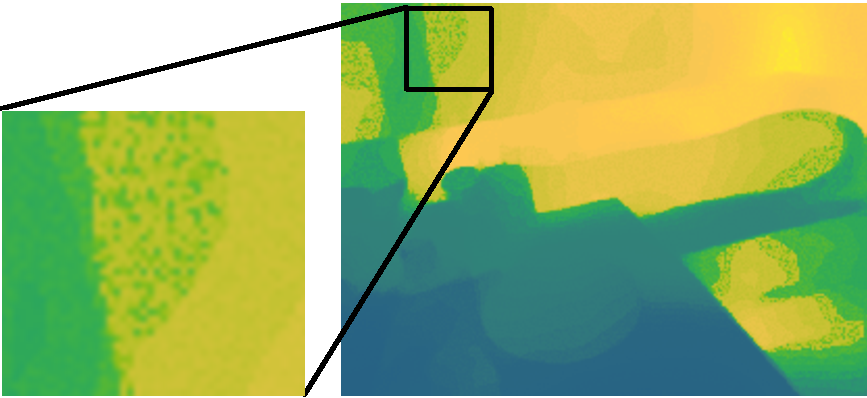
\includegraphics[width=0.66\textwidth]{dither.pdf}
  \caption{Example of dither artifacts. Sometimes, when our histogram matching
    is applied to images with large regions of similar depths, dither artifacts
    will occur.}
  \label{fig:dither}
\end{figure}


\section{Comparison of diffused vs. scanned imaging}
In our experiments, we capture measurements by scanning the scene with a
single-pixel SPAD detector whose optical path is aligned with a laser. This
arrangement allows us to capture a reference ``ground truth'' depth map for
quantitative validation of our method. To emulate measurements captured using a
system where the laser and detector are diffused over the scene, we digitally
sum the measurements to obtain a single transient. 

In order to verify that digital summation of scanned measurements yields results
that are similar to those captured by a diffused laser and detector, we capture
an example scene using a modified hardware prototype in both scanned and
diffused modes. The hardware prototype (shown in Fig.~\ref{fig:hardware})
consists of a more powerful laser (Katana 05HP, 532 nm) which we operate at
approximately 25 mW output power with two single-pixel SPAD detectors. One SPAD
is aligned with the optical path of the laser, and the other SPAD is operated
without a lens to integrate light from the entire scene. Both SPADs are fitted
with a 10 nm bandpass filter centered at 532 nm, which reduces the amount of
integrated ambient light. We attach a holographic diffuser (Thorlabs ED1-S50) to
the laser output in order to diffuse light onto the scene or alternatively
remove the diffuser and use a pair of scanning mirrors to scan the scene.

The modified hardware setup is used to capture an example scene in both scanned and
diffused modes, and the resulting transients are used to refine an initial depth
estimate from the Kinect RGB image. We illustrate the results of this procedure
in Fig.~\ref{fig:comparison}. The reconstructions from the scanned and diffused
measurements are similar in reconstruction quality and also show similar
quantitative improvement in terms or error over the initial depth estimate. The
normalized photon counts are also shown in Fig.~\ref{fig:comparison}, and we
note that the counts show similar trends. The number of recorded photons in
these experiments is shown in Table~\ref{tab:photon_counts}. In both cases, the
rate of detected photons is far less ($<$5\%) than the number of emitted laser
pulses, and so we conclude that the measurements are captured in the low-flux
regime where pileup effects are negligible. We attribute most of the differences
between the scanned and diffused transients to the baseline between the
positions of the diffused and scanned SPADs (see Fig.~\ref{fig:hardware}).

\begin{figure}[H]
  \centering \includegraphics[width=\textwidth]{diffused_hardware/setup.pdf}
  \caption{Modified hardware setup. The setup is used to compare scanned and
  diffused measurements and employs two SPAD detectors and two laser
  configurations. In the first configuration, the scene is illuminated by
  sending the laser light through a holographic diffuser and a lensless SPAD 
  integrates light from the entire scene. In the second, the SPAD is aligned
  with the optical path of the laser and the scene is scanned using a pair of
  scanning mirrors. The baseline between the two SPADs (right) results in some
  observed differences in the recorded transients.}
  \label{fig:dither}
\end{figure}

\begin{table}[ht!]
    \renewcommand{\arraystretch}{1.3}
    \setlength{\tabcolsep}{10pt}
     \centering
     \begin{tabular}{lccc} \toprule
         \textbf{Experiment} & \textbf{Detected Photons} & \textbf{Laser Pulses} & \textbf{Detection Rate} \\\hline
         \textbf{Scanned} & XXX & $6\times10^7$ & XXX \\
         \textbf{Diffused} & XXX & $6\times10^7$ & XXX \\
        \bottomrule
    \end{tabular}
    \vspace{0.4em}
    \caption{\textbf{Recorded photons for diffused vs. scanned scene.} In each capture mode, scanned or diffused, the number of detected photons does not exceed 5\% of the number of emitted laser pulses, placing the capture within the low-flux regime where pileup effects are negligible.}
    \label{tab:photon_counts}
\end{table}

\section{Additional results on NYU Depth v2}
Figures \ref{fig:densedepth_1}--\ref{fig:midas_3} show additional results
for our method on the NYU Depth v2 dataset when the depth estimate is
initialized with the DenseDepth \cite{Alhashim2018} (Figures
\ref{fig:densedepth_1}--\ref{fig:densedepth_3}), DORN \cite{Fu2018} (Figures
\ref{fig:dorn_1}--\ref{fig:dorn_3}) 
and MiDaS \cite{Lasinger:2019} (Figures \ref{fig:midas_1} -- \ref{fig:midas_3}) monocular depth estimators.

We compare the output of the network $z_0$, the
median-rescaled network output (where the depth map $z_0$ is scaled pixel-wise by a
scalar $\frac{\text{median}(z_{GT})}{\text{median}(z_0)}$, $z_{GT}$ being the
ground truth depth map), the network output matched to the ground truth depth histogram, and the output of
our histogram matching method under a signal-to-background ratio (SBR) of 100.
We use the luminance of the RGB image as our reflectance map
for both SPAD simulation and histogram matching.
We show absolute difference maps and also give
the root-mean-square error (RMSE) for each example.
% \begin{figure}[H]
%   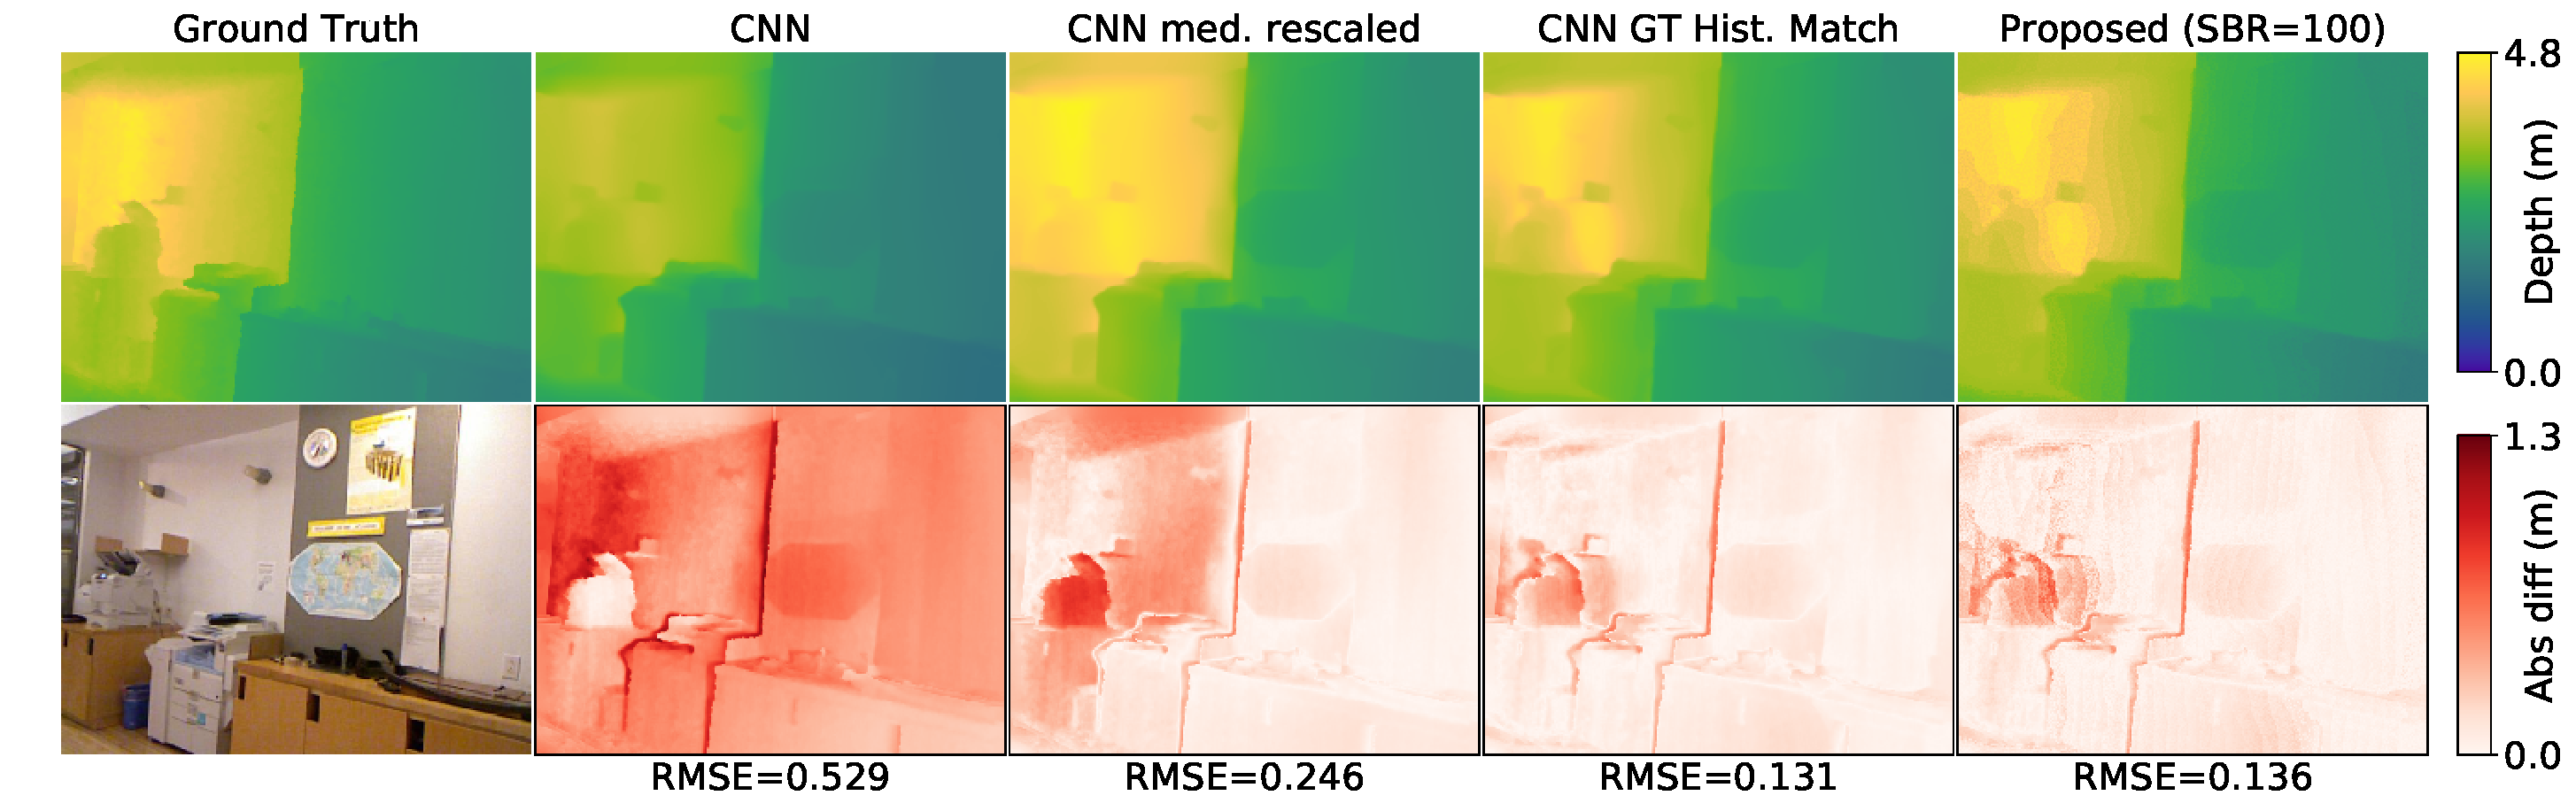
\includegraphics[width=\textwidth]{comparison/densedepth_18_comparison.pdf}
%   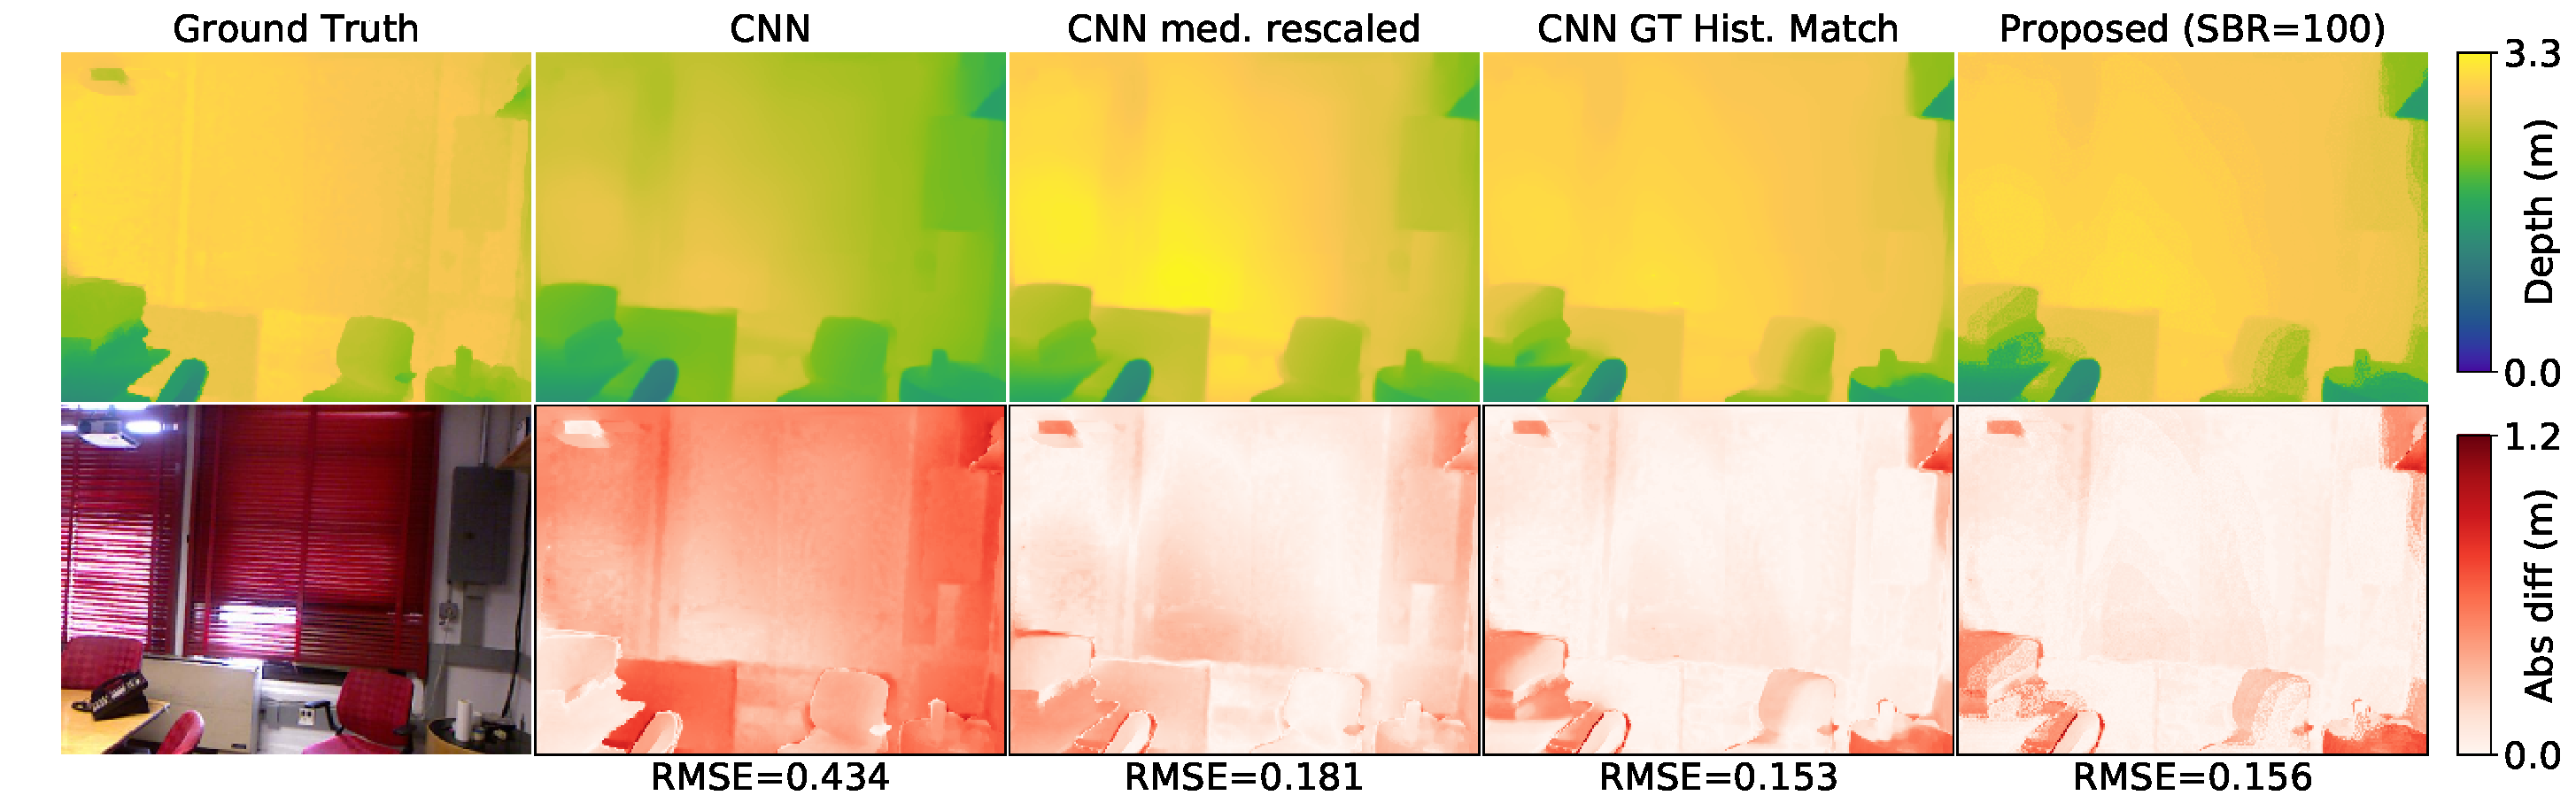
\includegraphics[width=\textwidth]{comparison/densedepth_21_comparison.pdf}
%   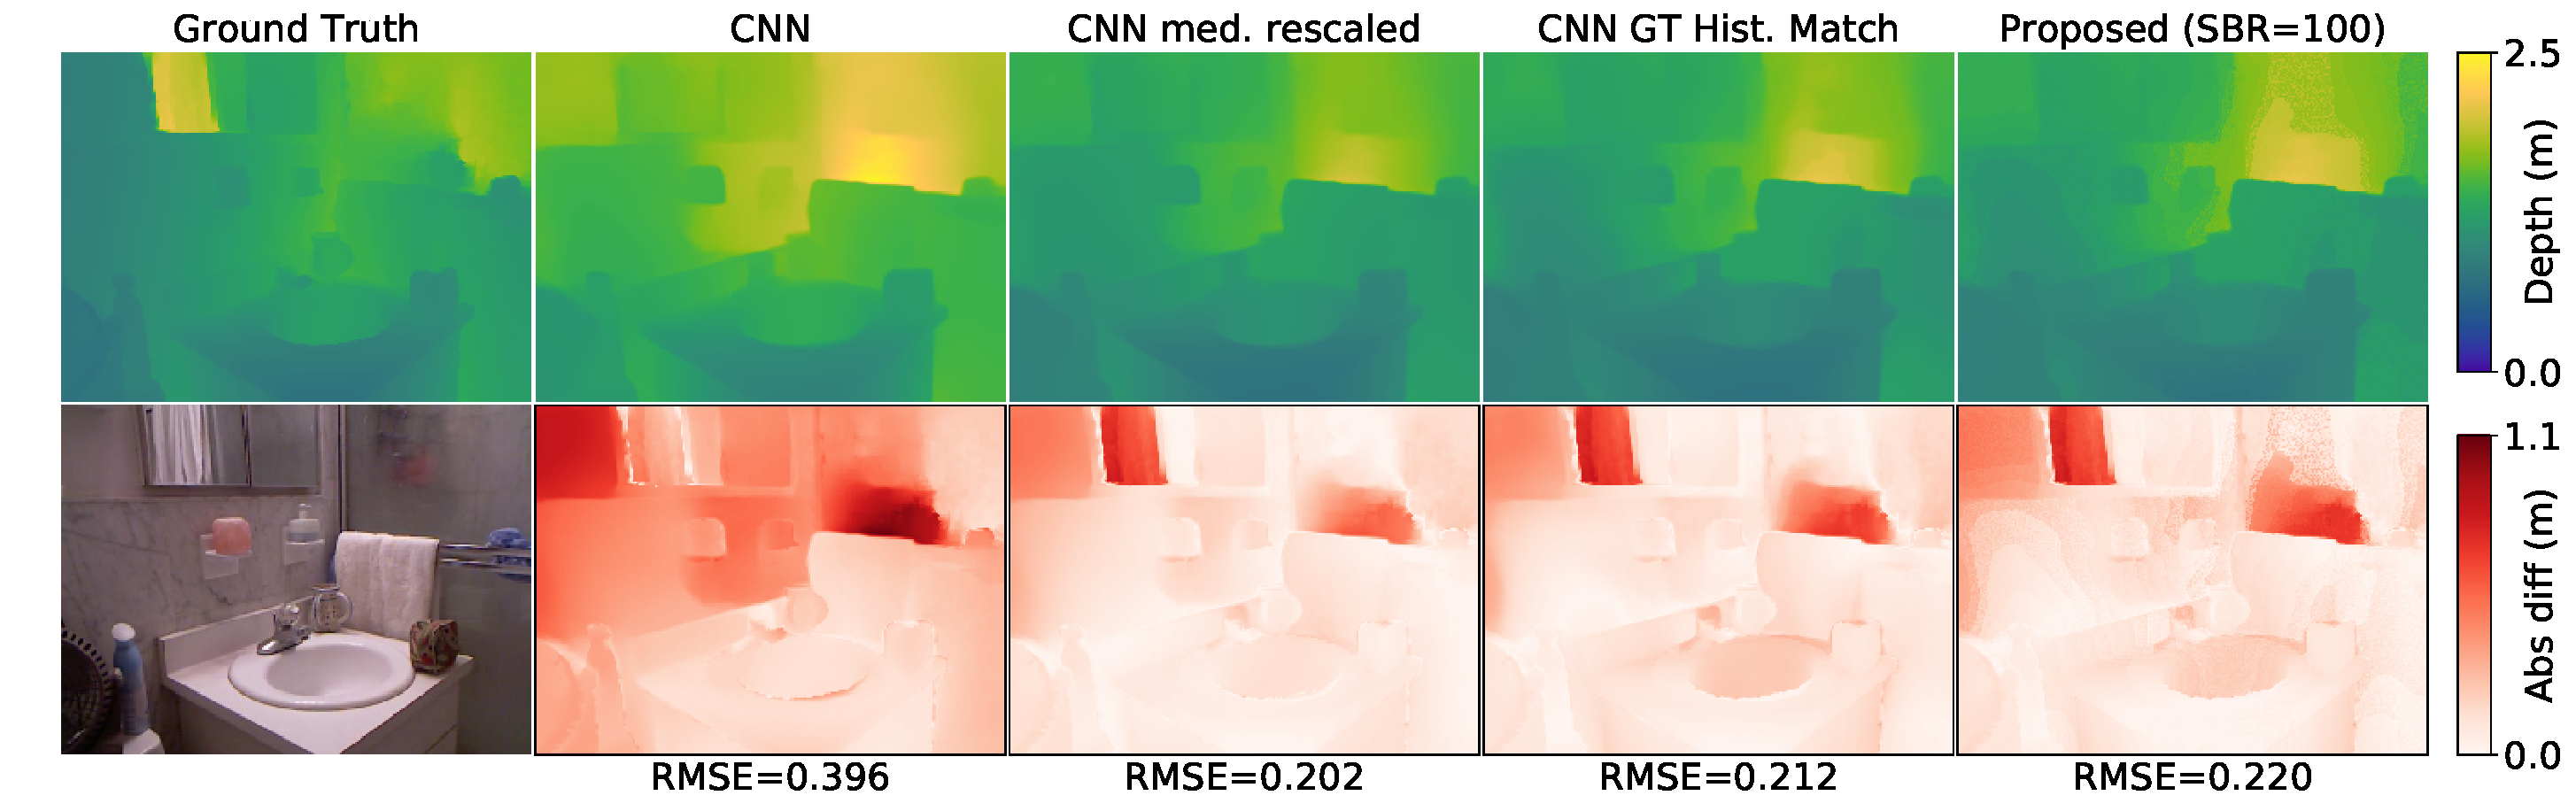
\includegraphics[width=\textwidth]{comparison/densedepth_25_comparison.pdf}
%   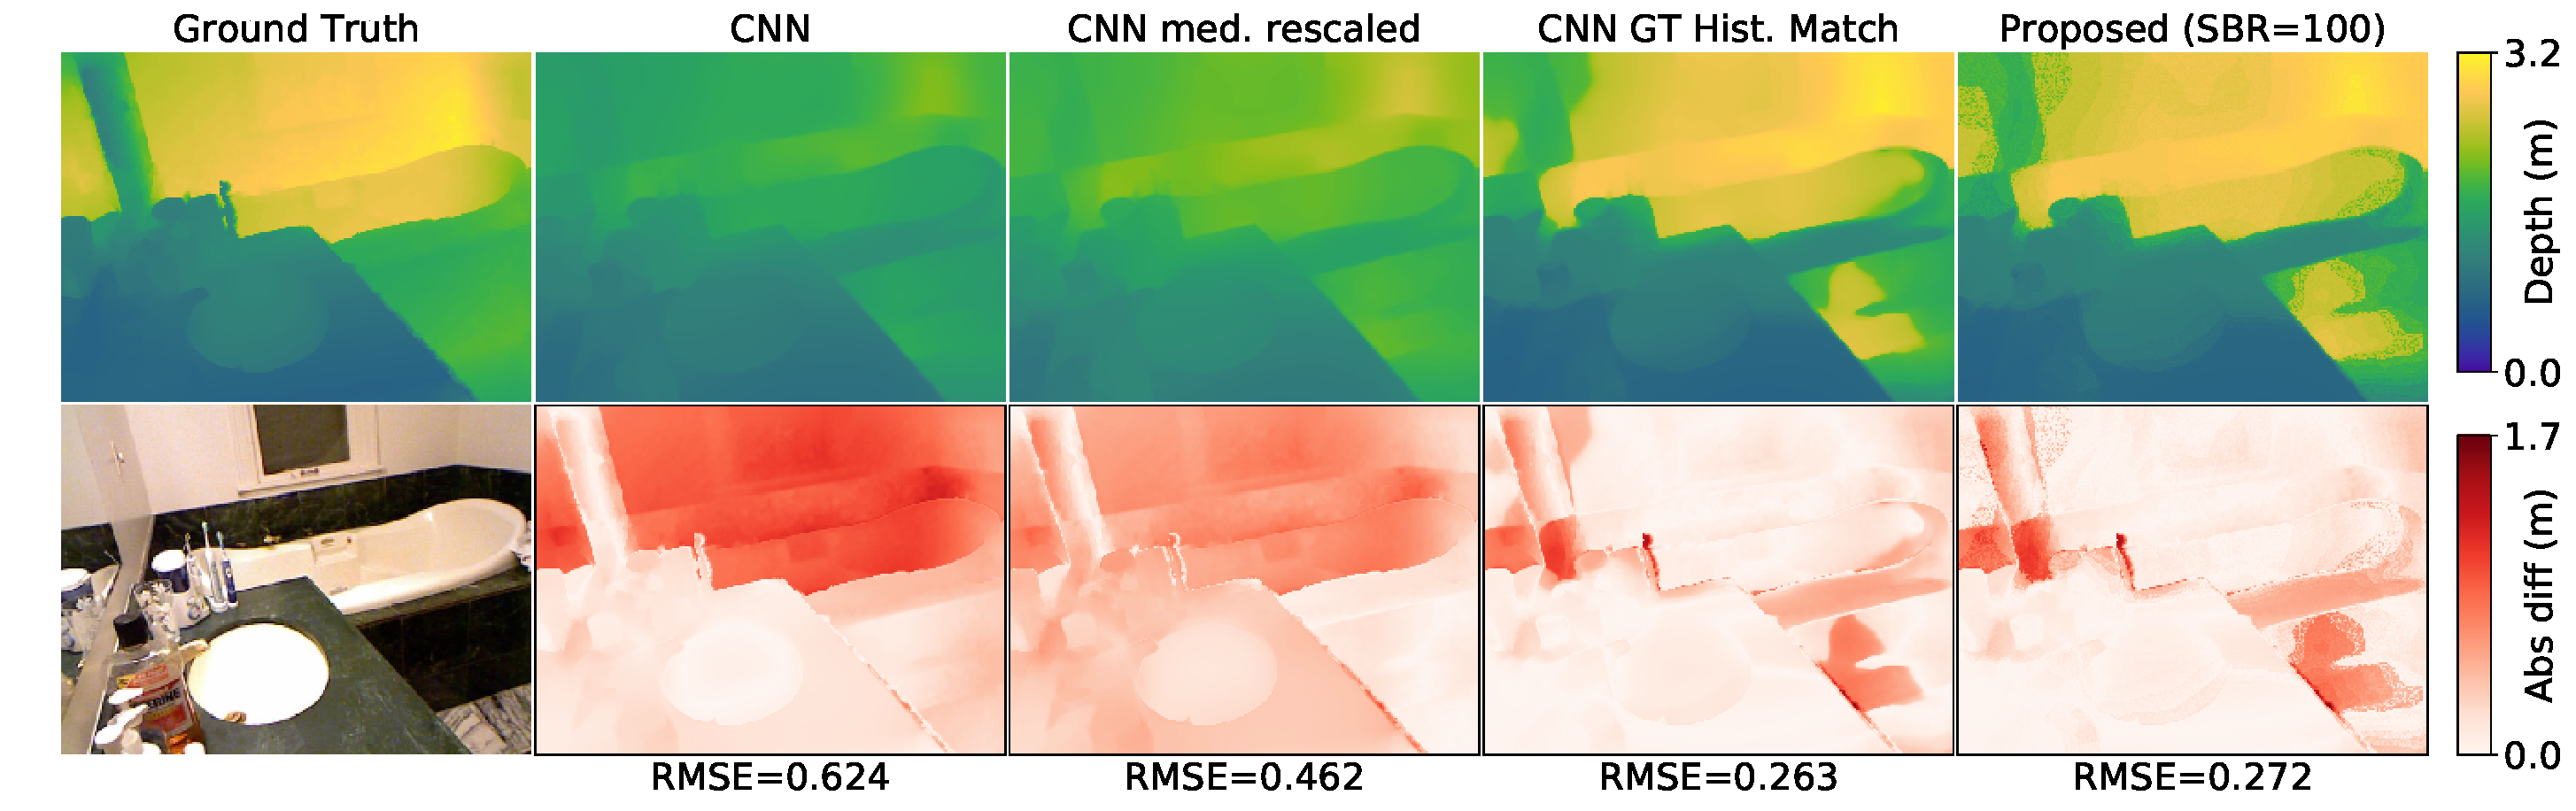
\includegraphics[width=\textwidth]{comparison/densedepth_194_comparison.pdf}
%   \caption{Results with DenseDepth as the MDE. Our method is able to scale and
%     shift the depth maps to mitigate gross errors in depth scaling.}
%   \label{fig:densedepth_1}
% \end{figure}
\begin{figure}[H]
  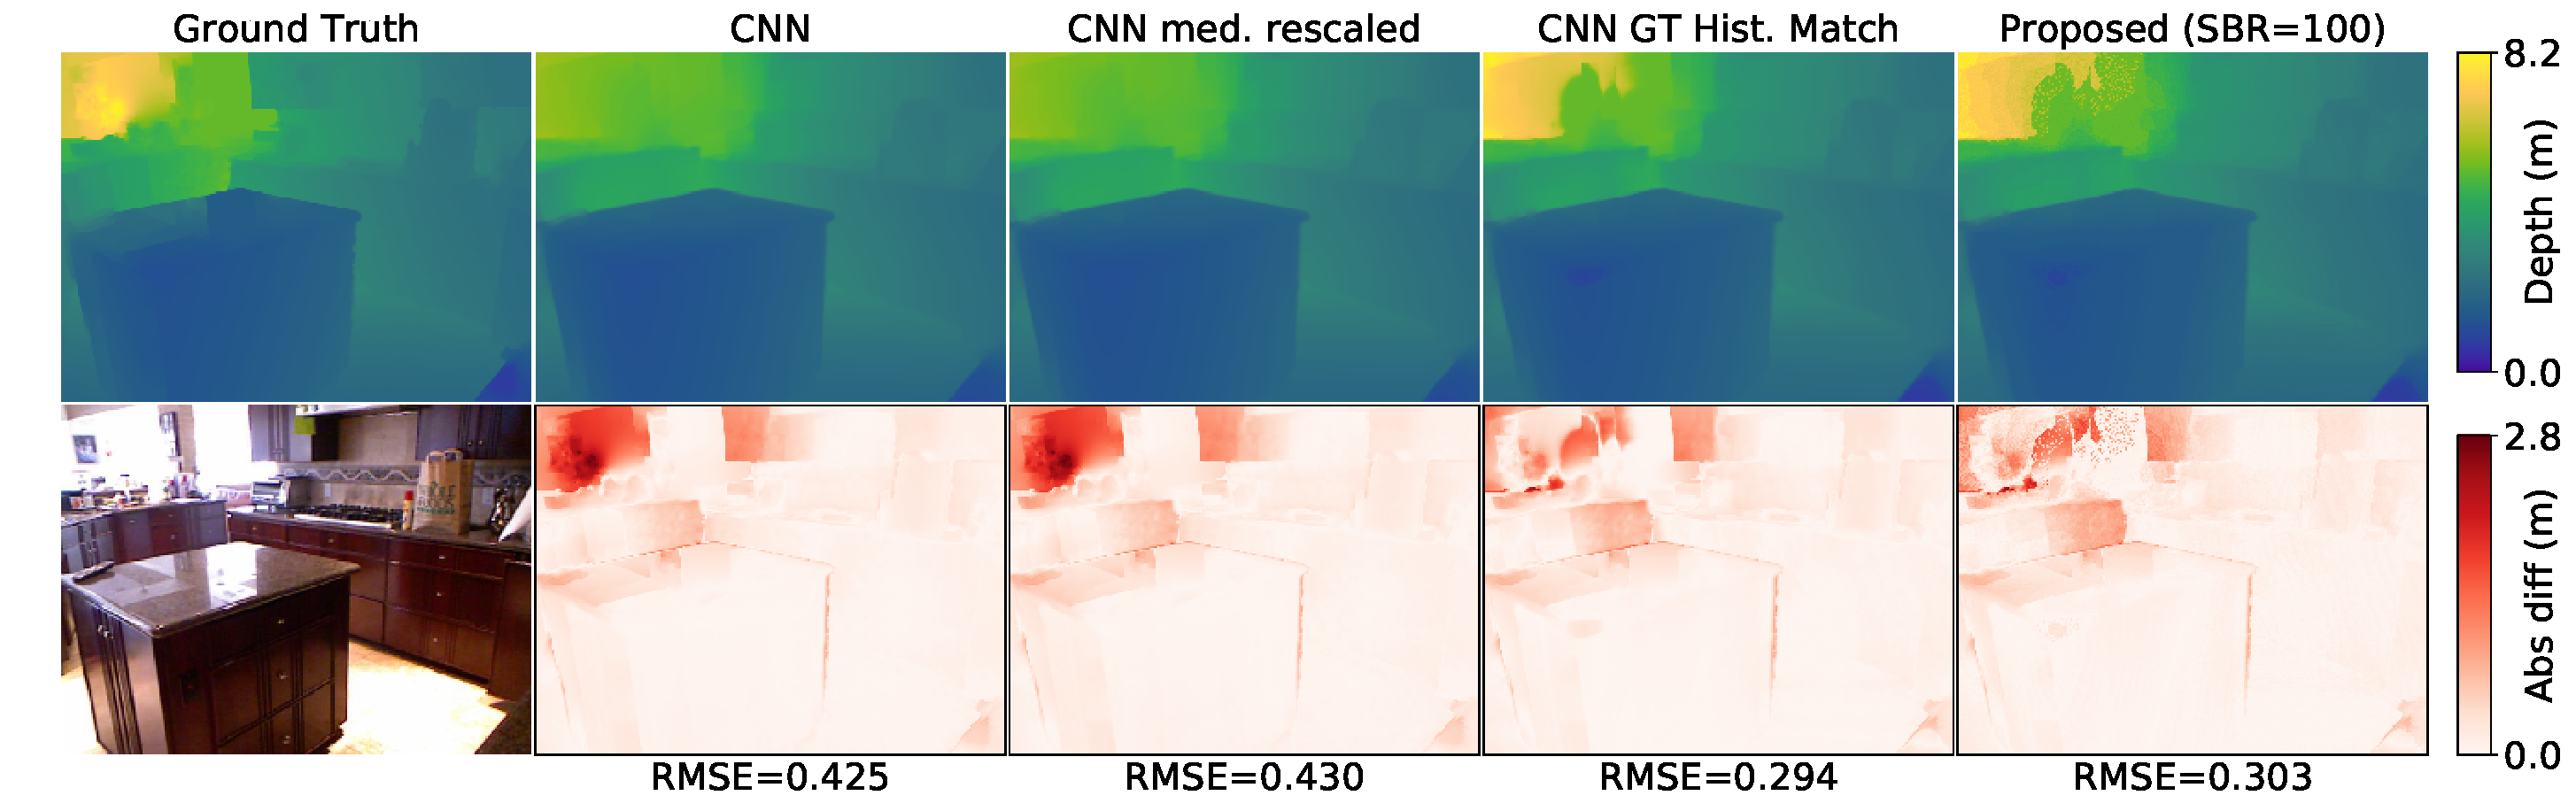
\includegraphics[width=\textwidth]{comparison/densedepth_362_comparison.pdf}
  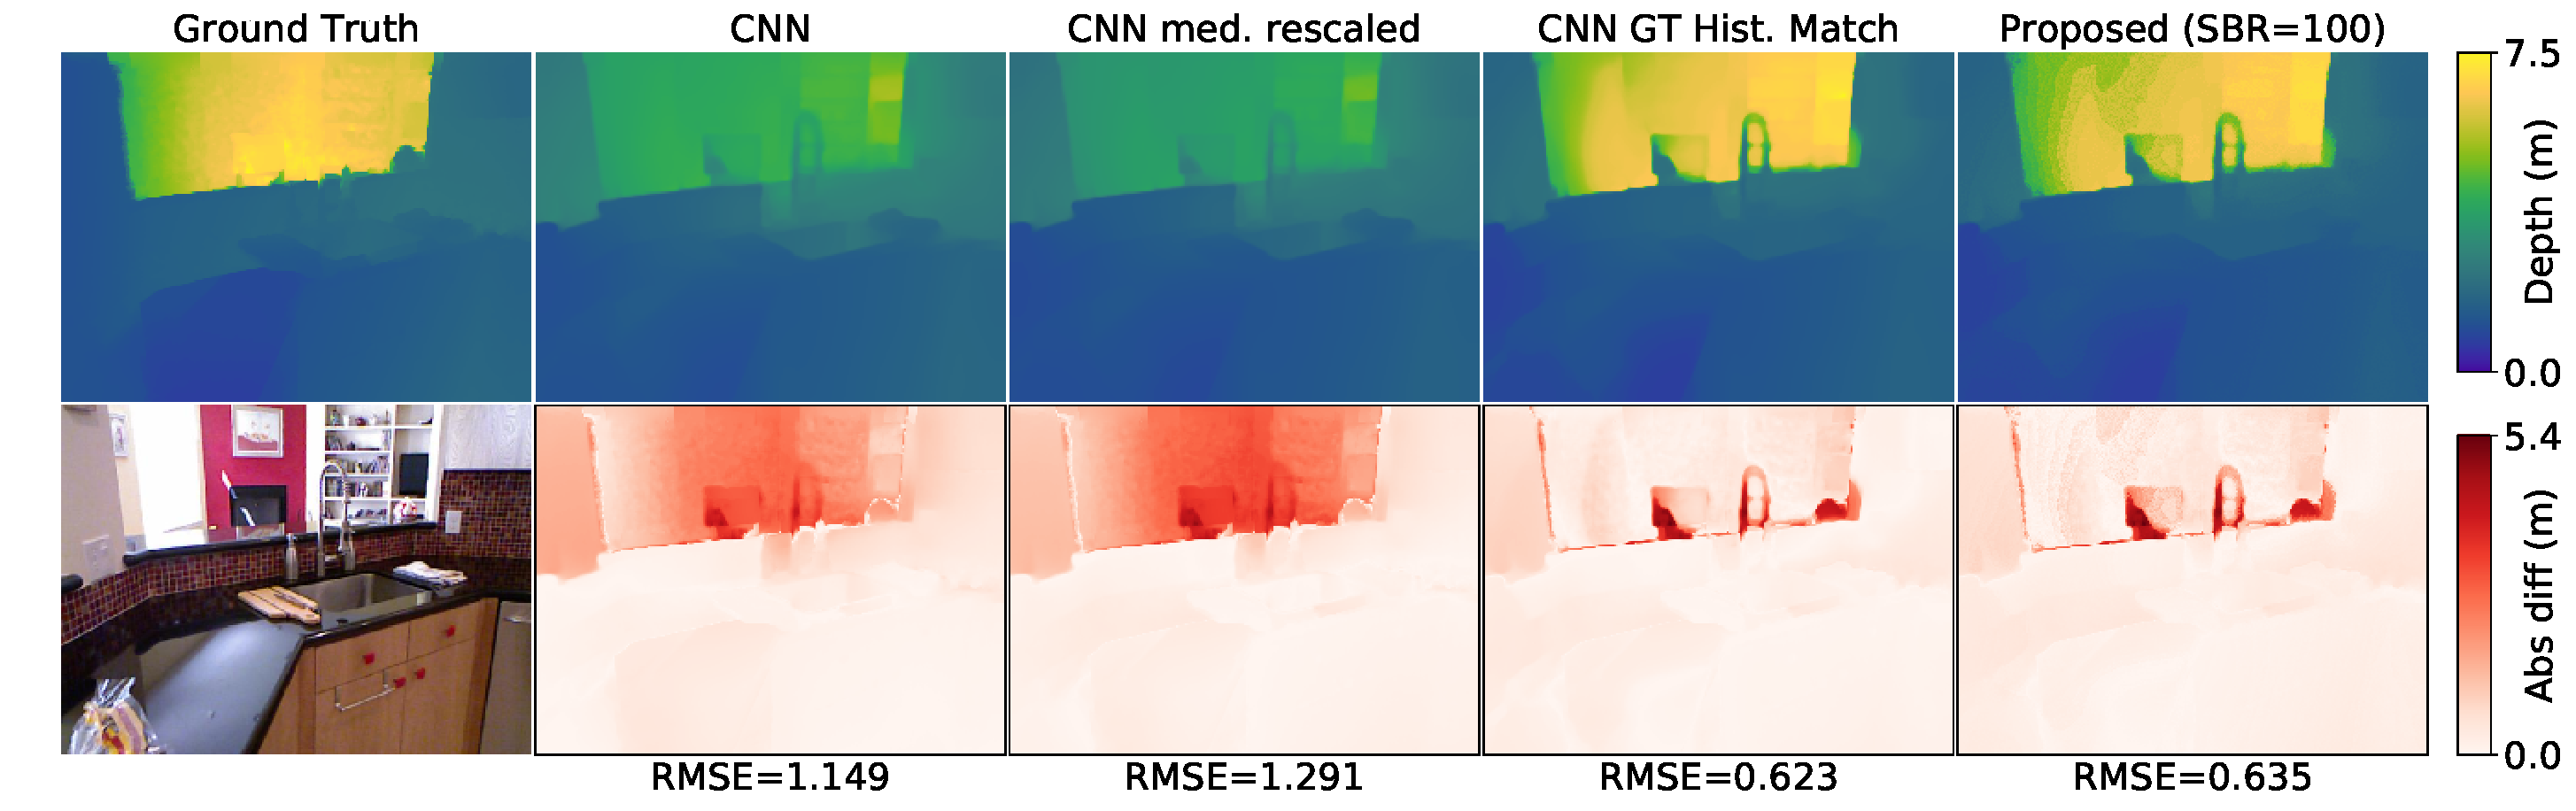
\includegraphics[width=\textwidth]{comparison/densedepth_379_comparison.pdf}
  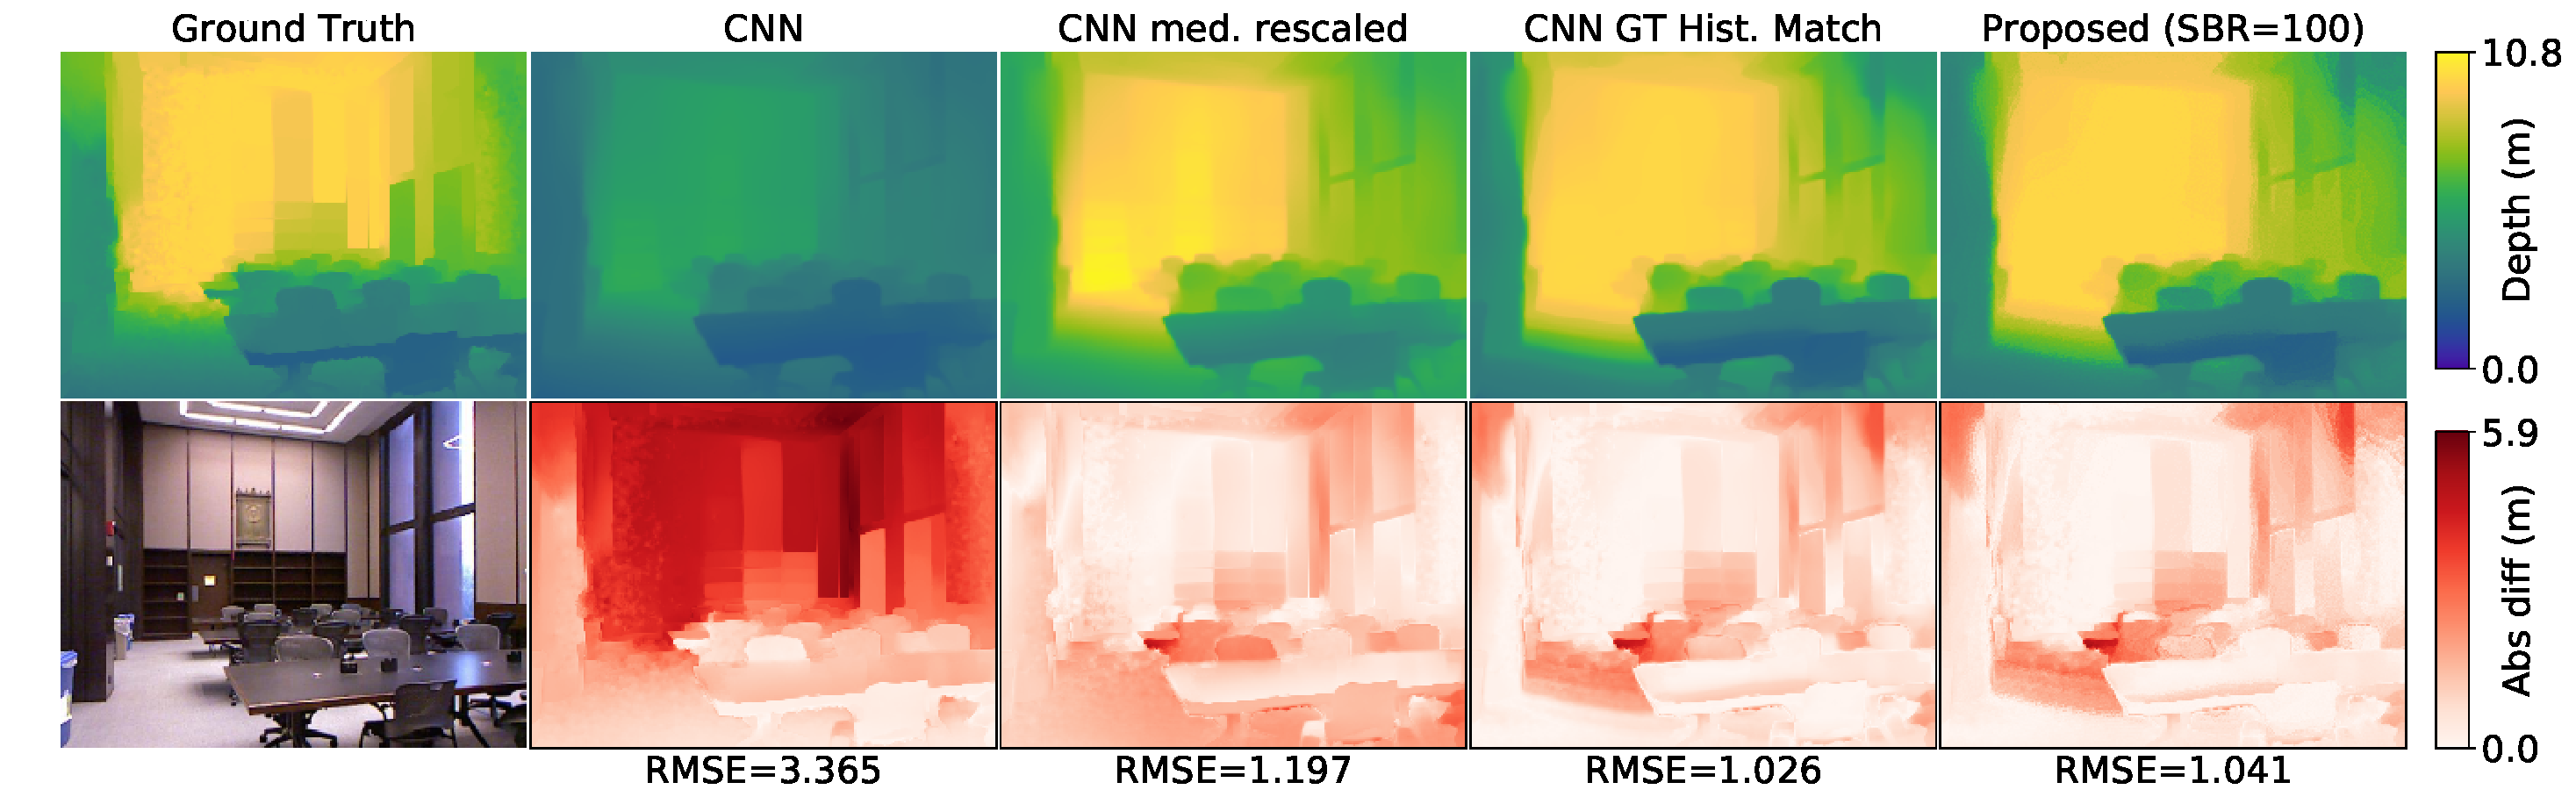
\includegraphics[width=\textwidth]{comparison/densedepth_107_comparison.pdf}
  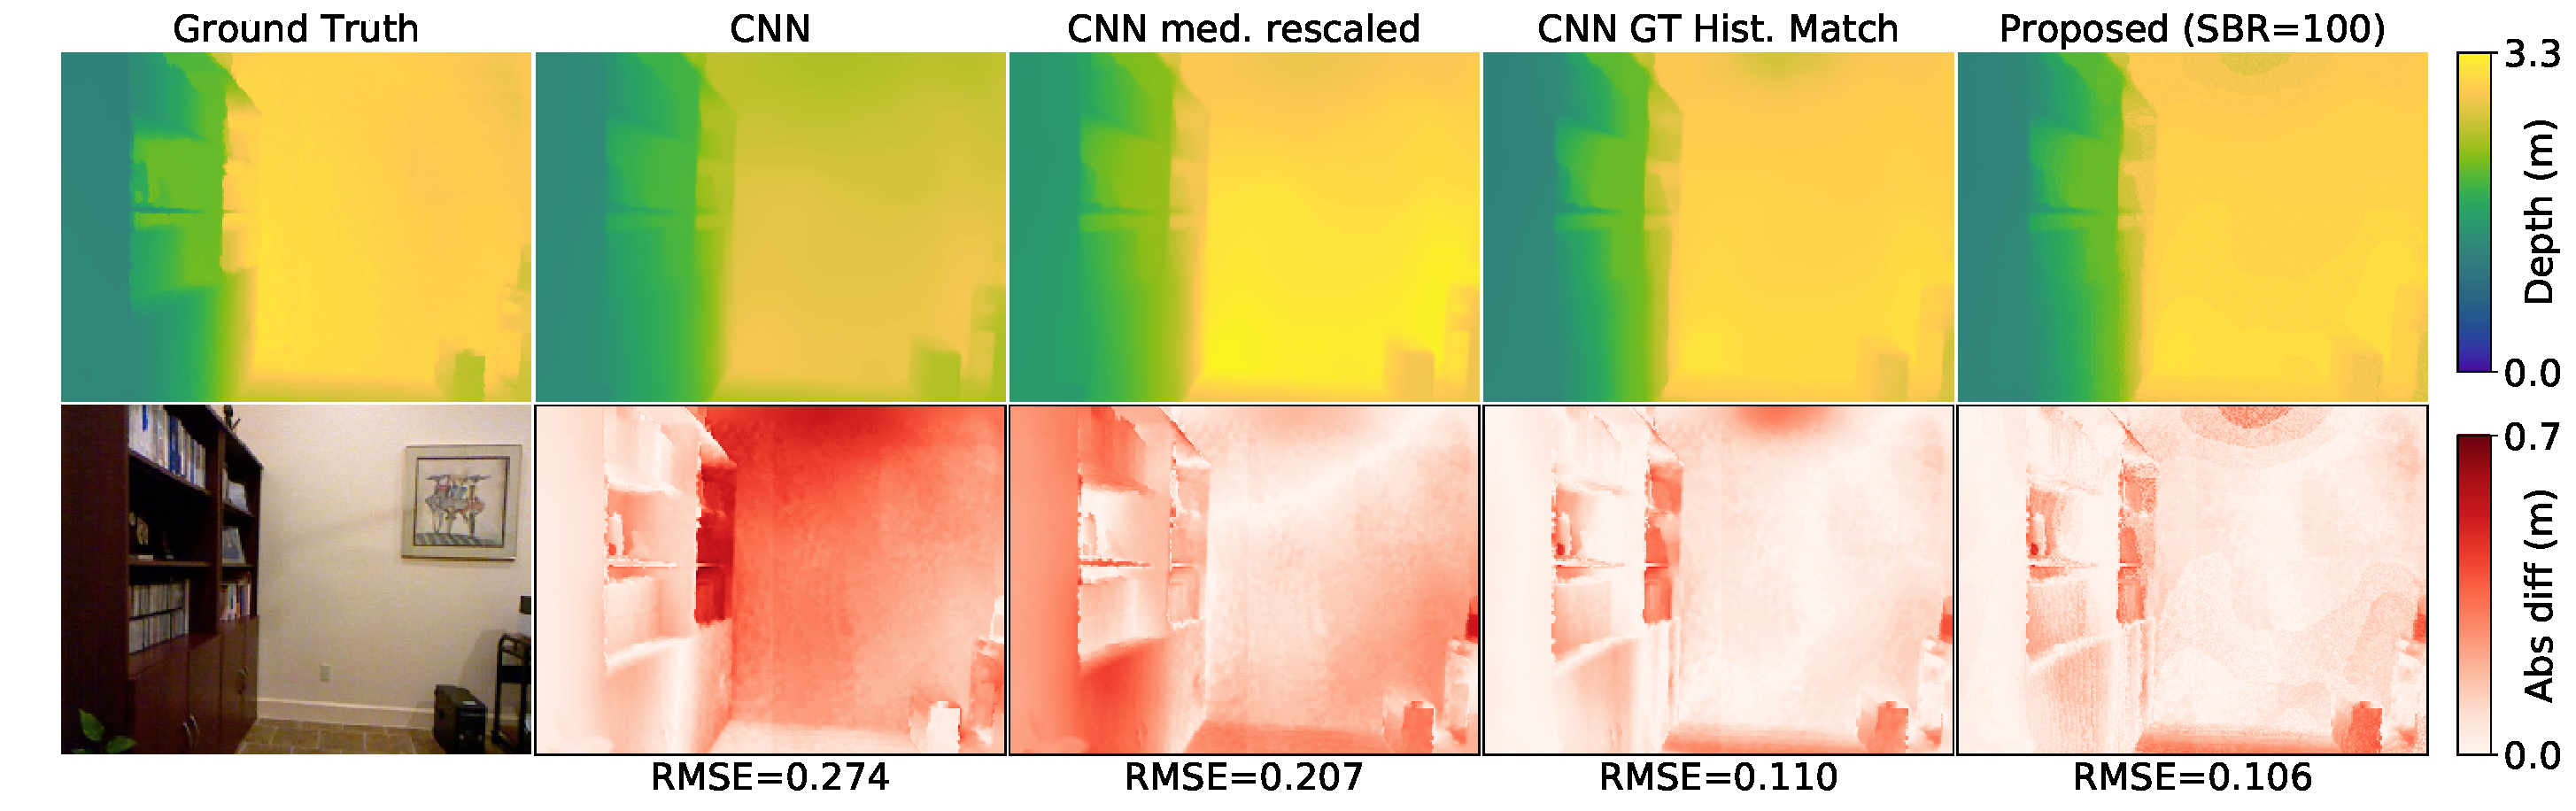
\includegraphics[width=\textwidth]{comparison/densedepth_187_comparison.pdf}
  \caption{Results with DenseDepth as the MDE. Our method is able to scale and
    shift the depth maps to mitigate gross errors in depth scaling.}
  \label{fig:densedepth_1}
\end{figure}
\begin{figure}[H]
  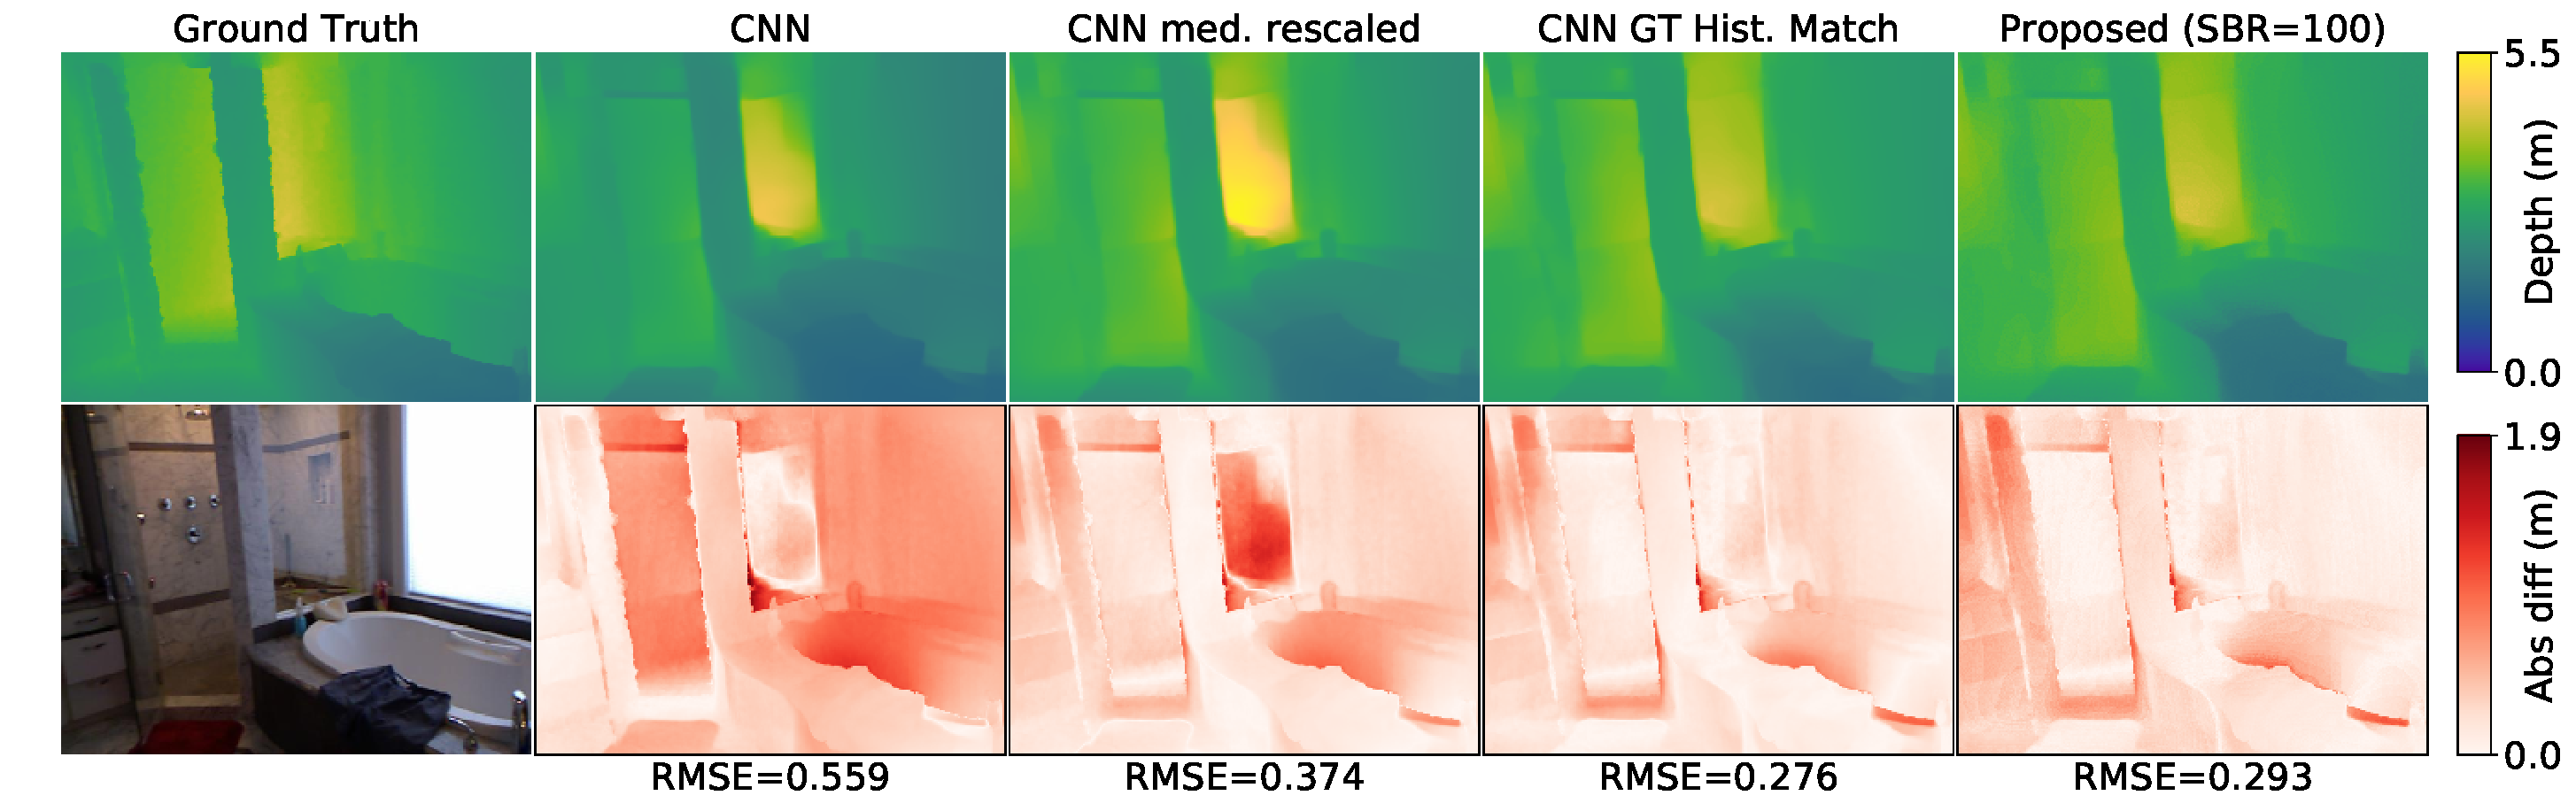
\includegraphics[width=\textwidth]{comparison/densedepth_285_comparison.pdf}
  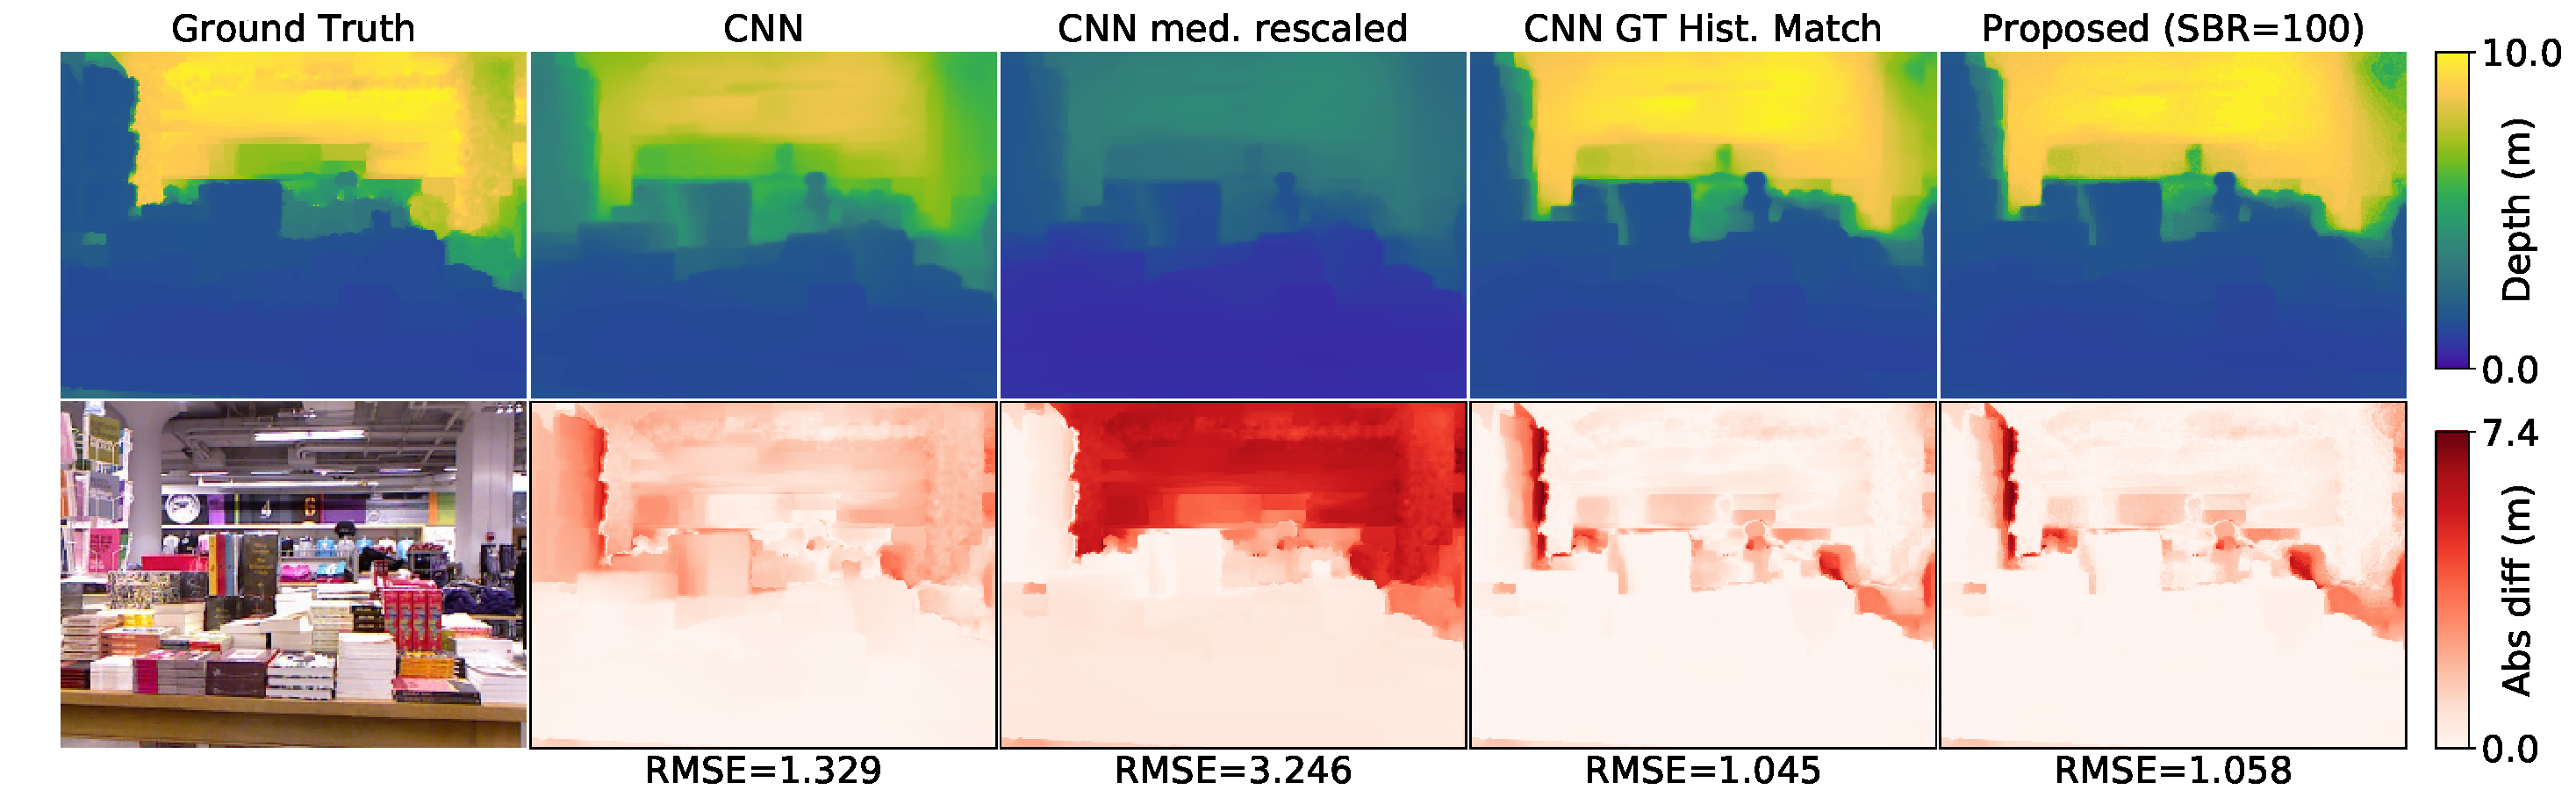
\includegraphics[width=\textwidth]{comparison/densedepth_42_comparison.pdf}
  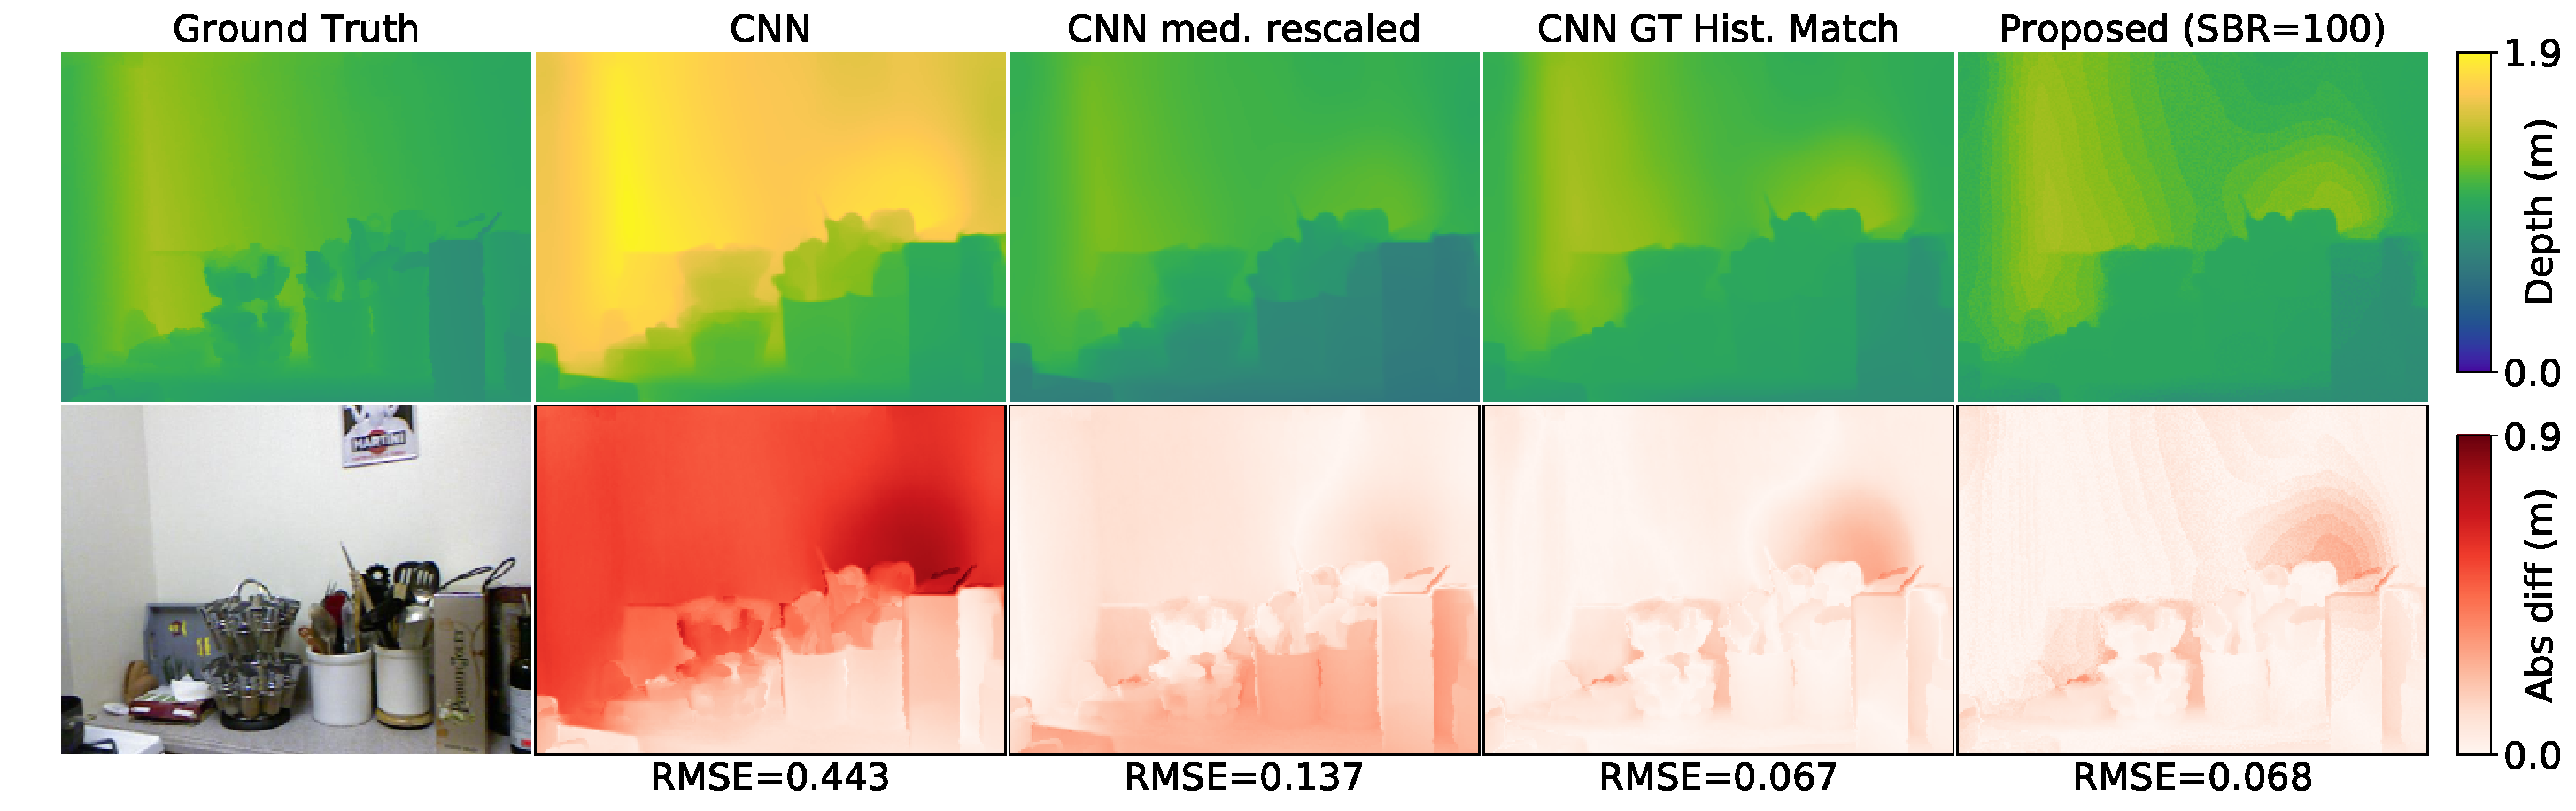
\includegraphics[width=\textwidth]{comparison/densedepth_52_comparison.pdf}
  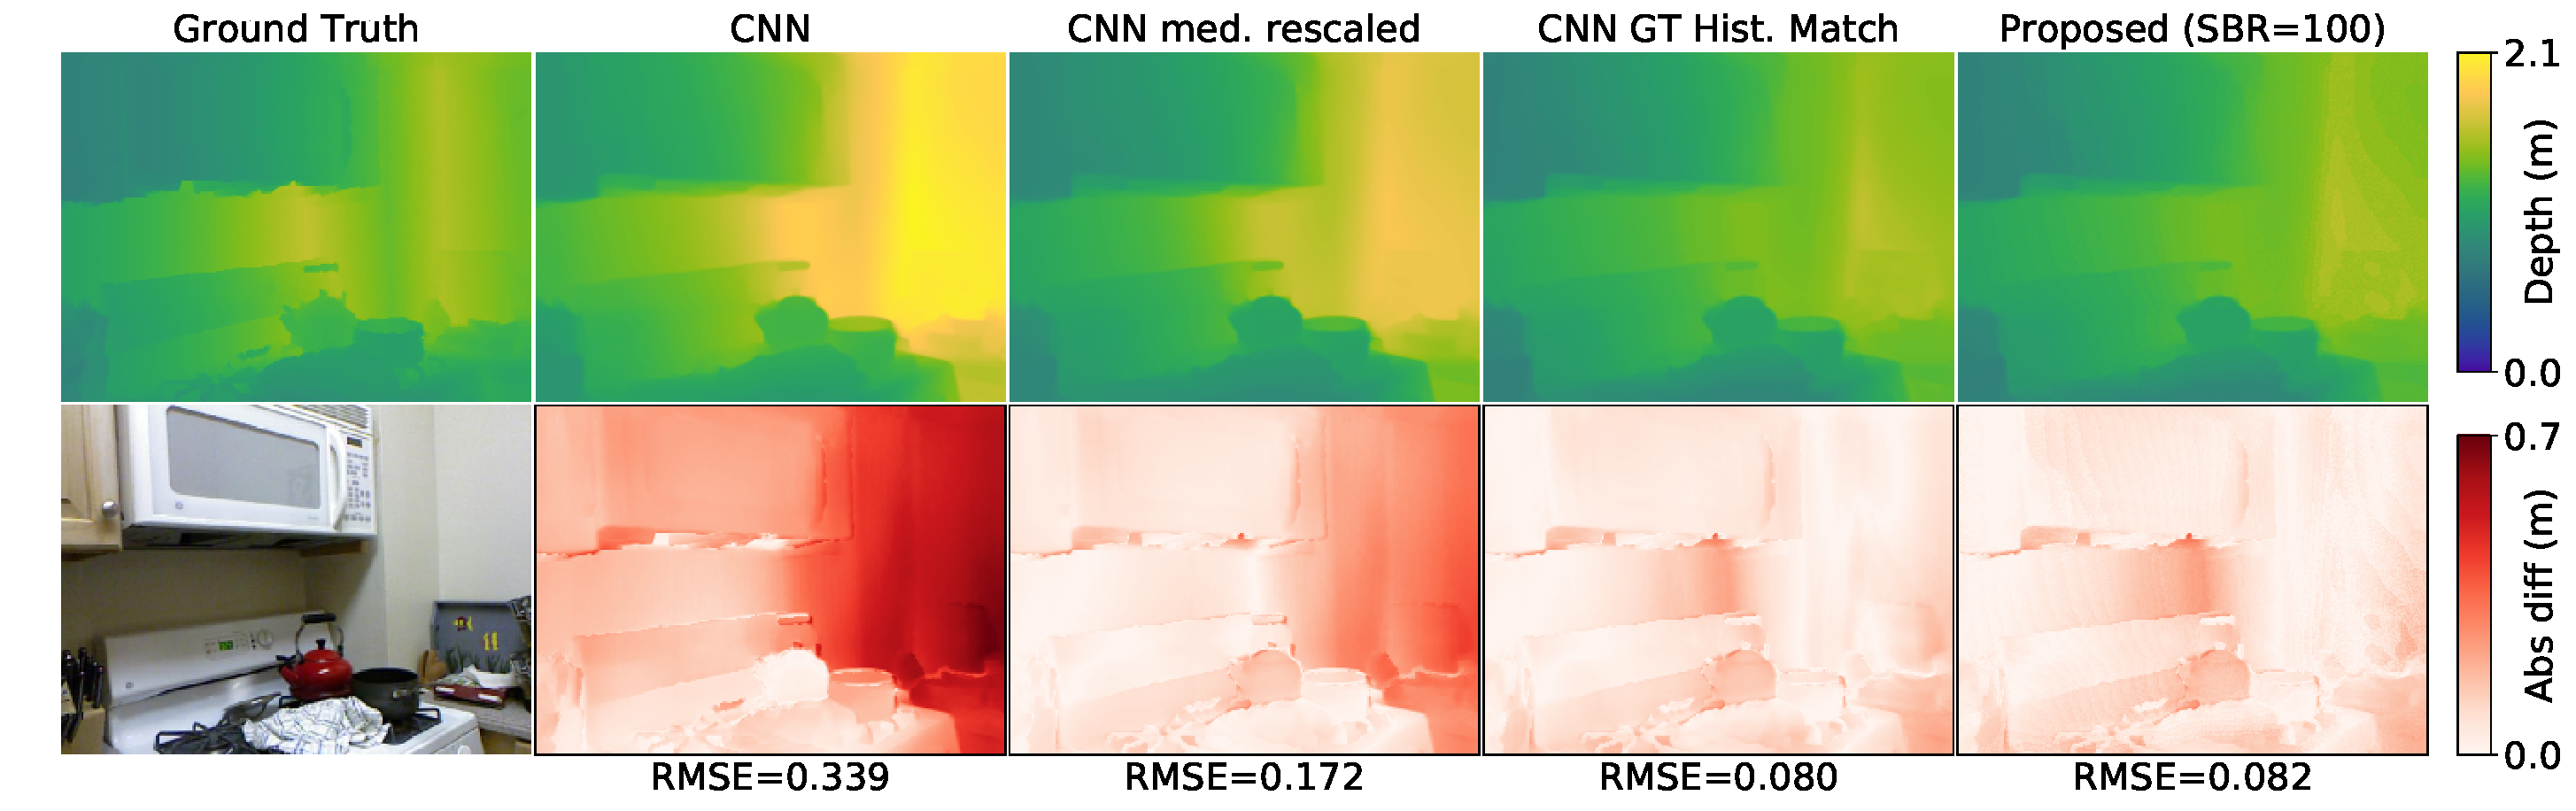
\includegraphics[width=\textwidth]{comparison/densedepth_53_comparison.pdf}
  \caption{Results with DenseDepth as the MDE. Our method is able to scale and
    shift the depth maps to mitigate gross errors in depth scaling.}
  \label{fig:densedepth_2}
\end{figure}
\begin{figure}[H]
  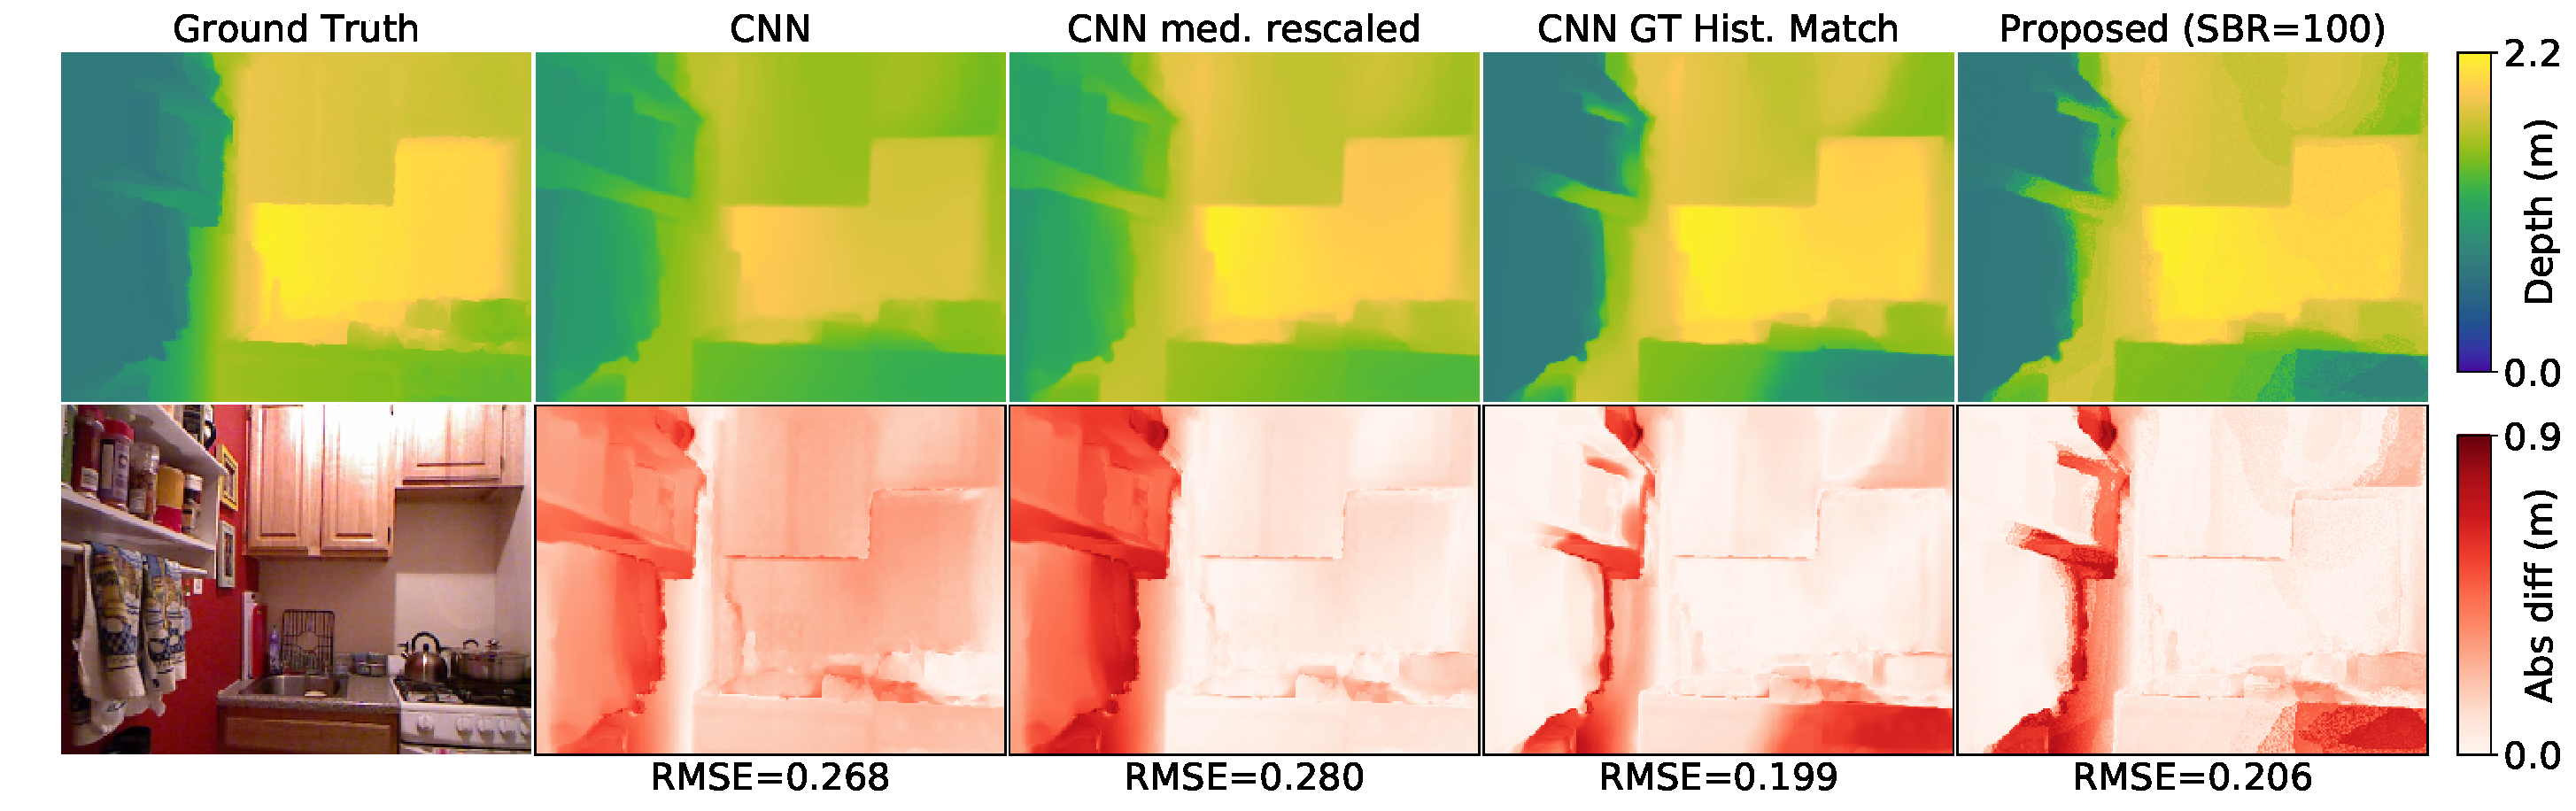
\includegraphics[width=\textwidth]{comparison/densedepth_103_comparison.pdf}
  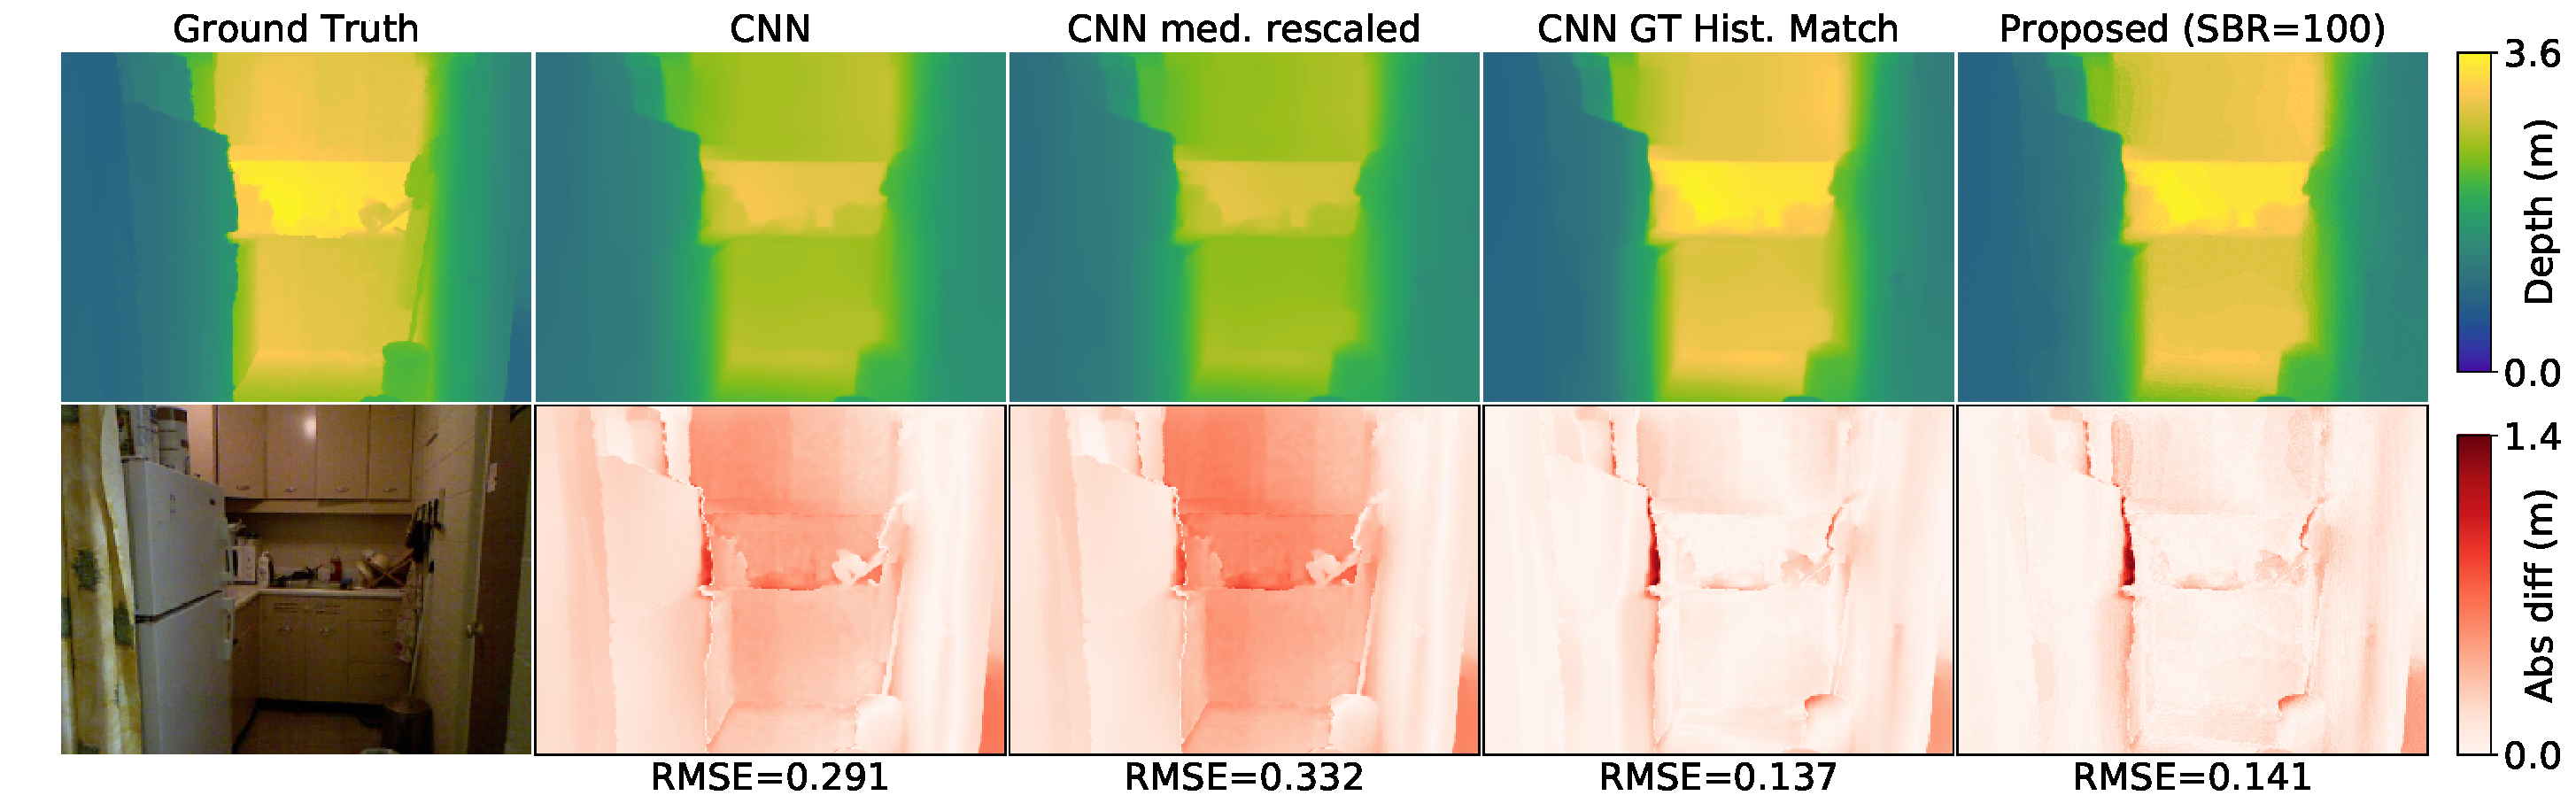
\includegraphics[width=\textwidth]{comparison/densedepth_224_comparison.pdf}
  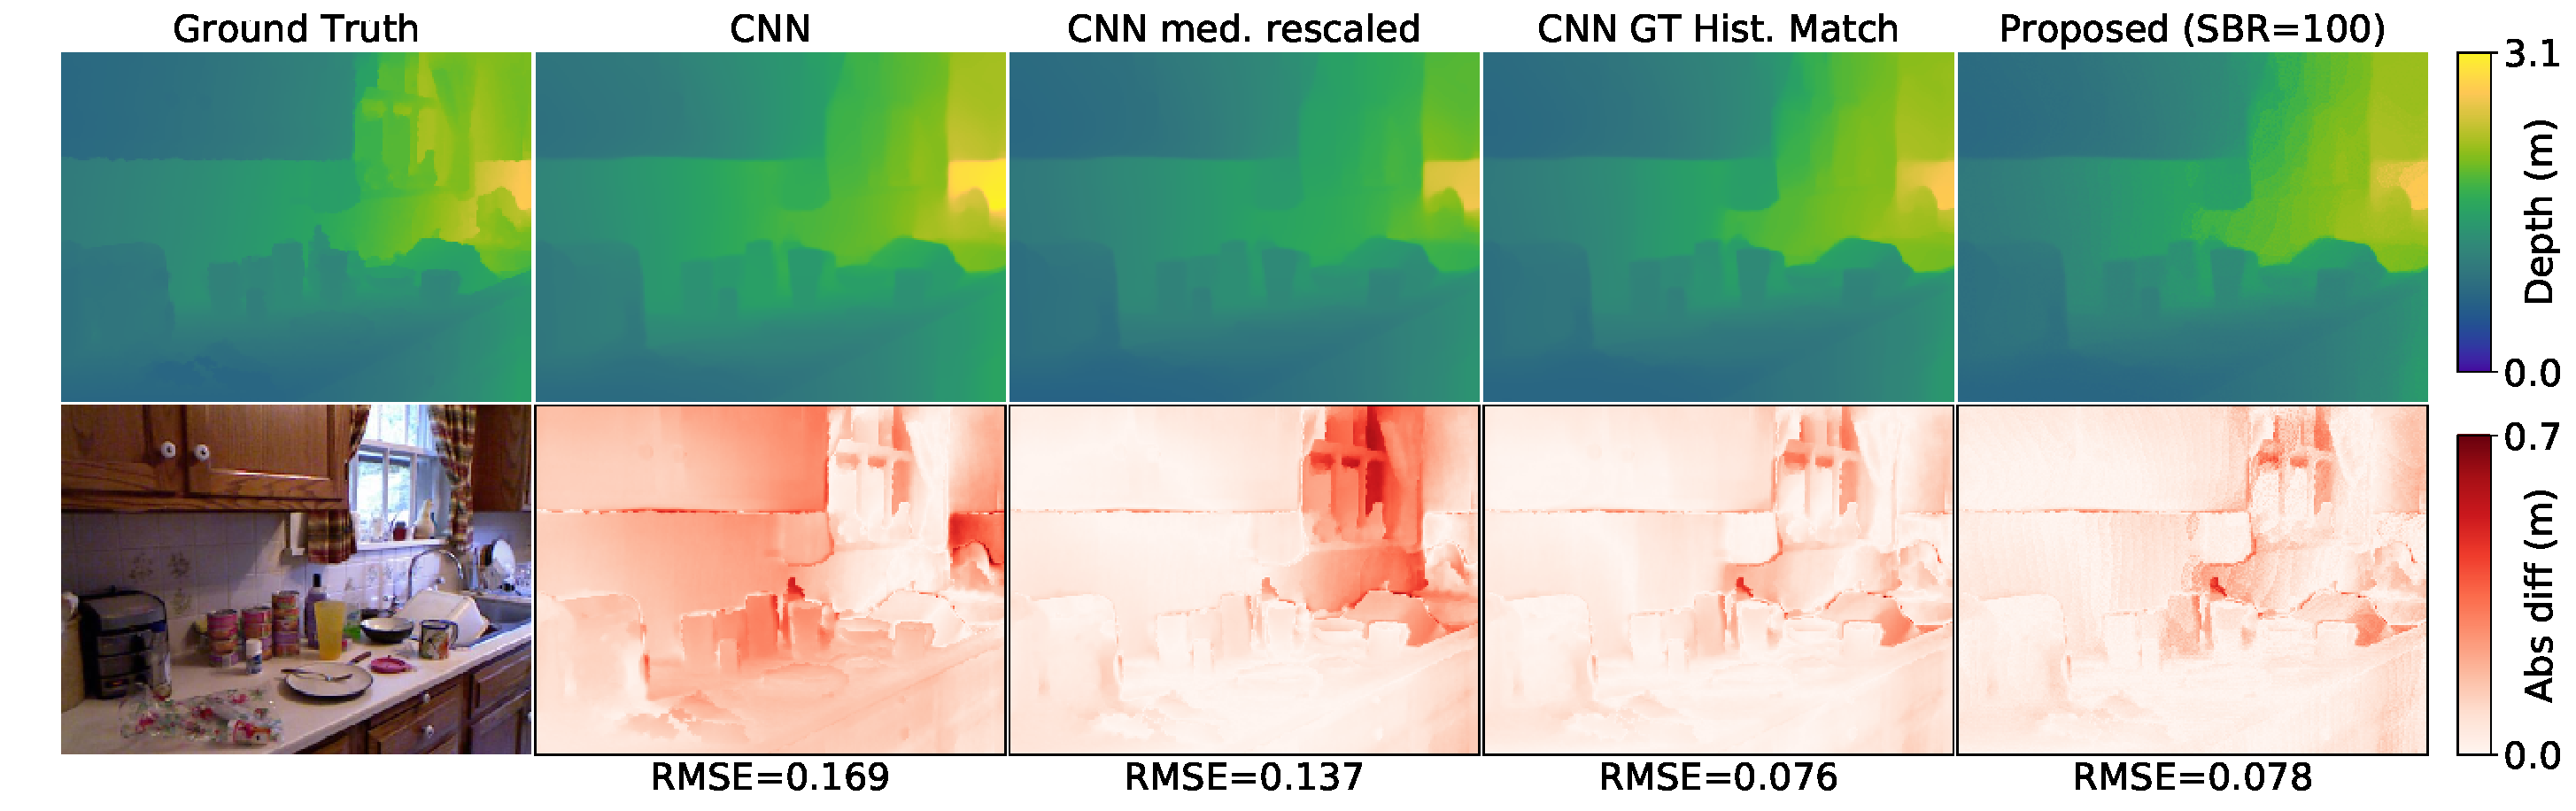
\includegraphics[width=\textwidth]{comparison/densedepth_226_comparison.pdf}
  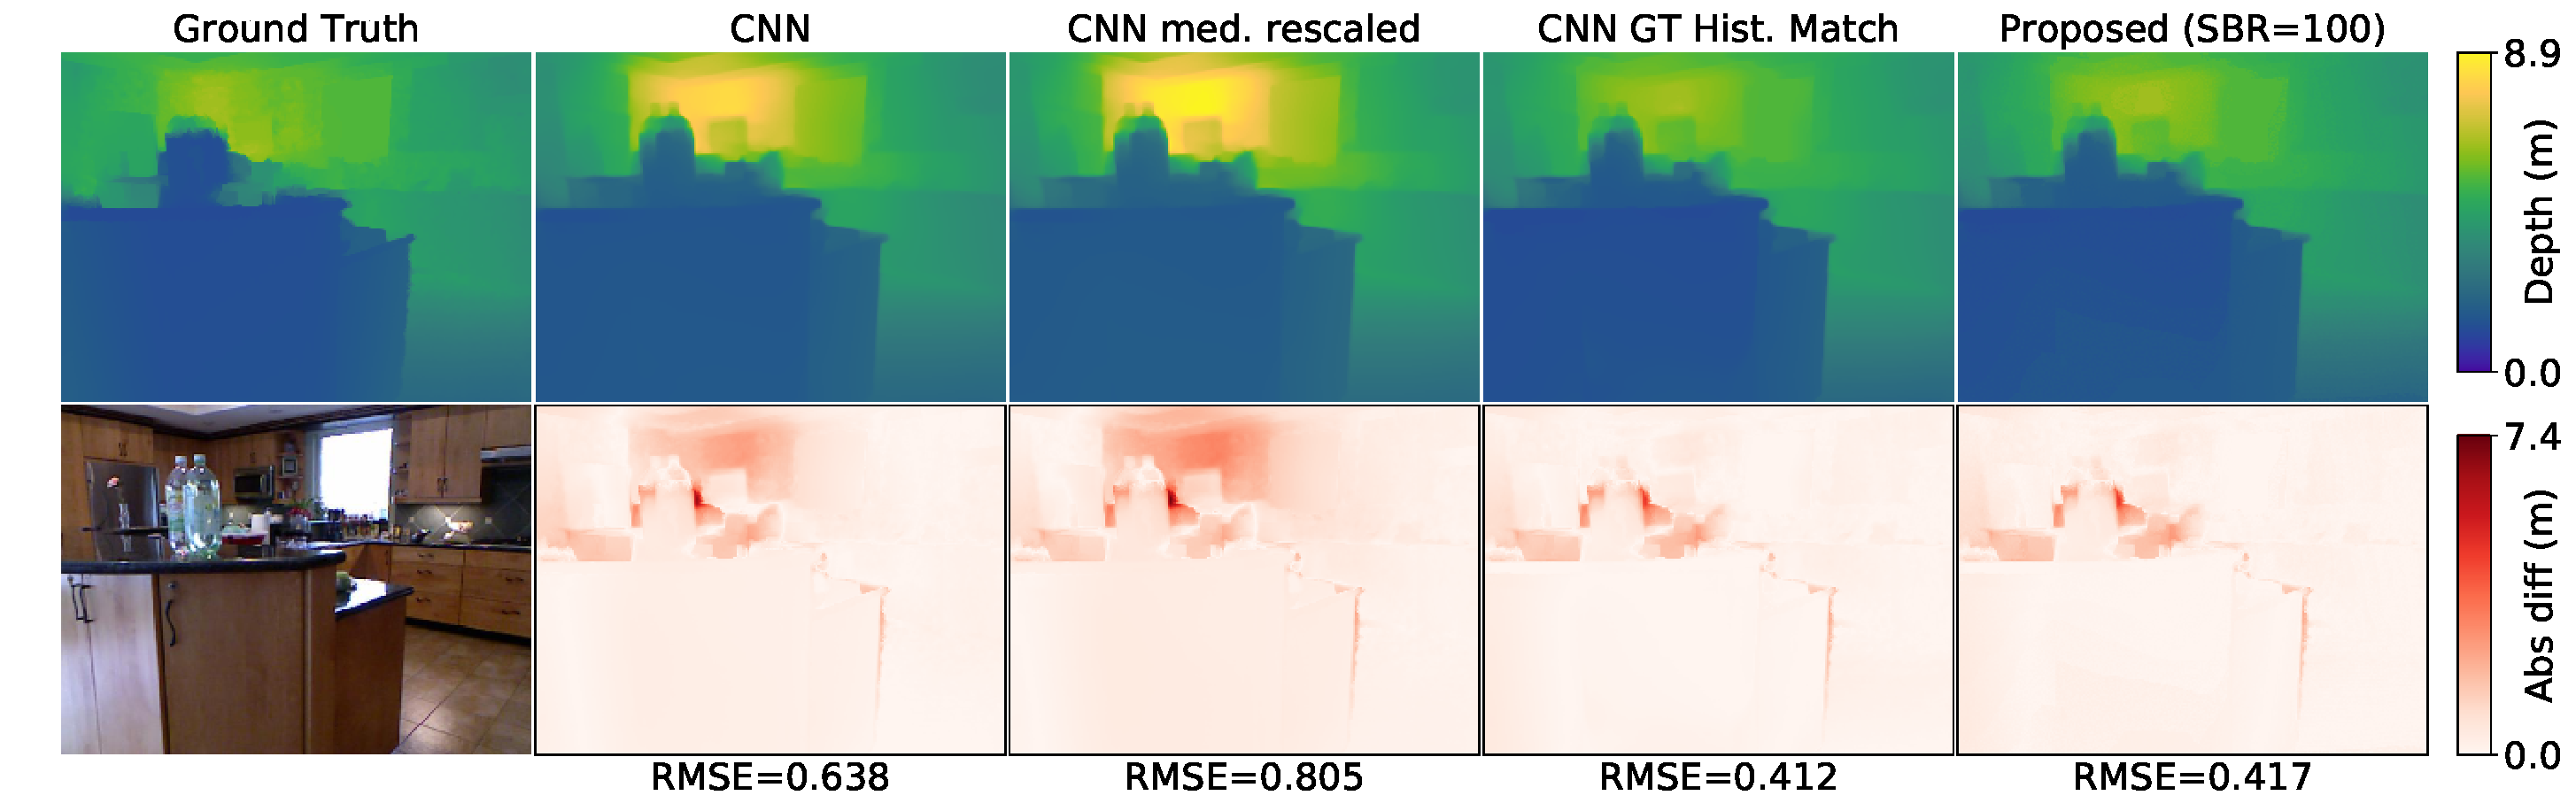
\includegraphics[width=\textwidth]{comparison/densedepth_352_comparison.pdf}
  \caption{Results with DenseDepth as the MDE. Our method is able to scale and
    shift the depth maps to mitigate gross errors in depth scaling.}
  \label{fig:densedepth_3}
\end{figure}
% \begin{figure}
%   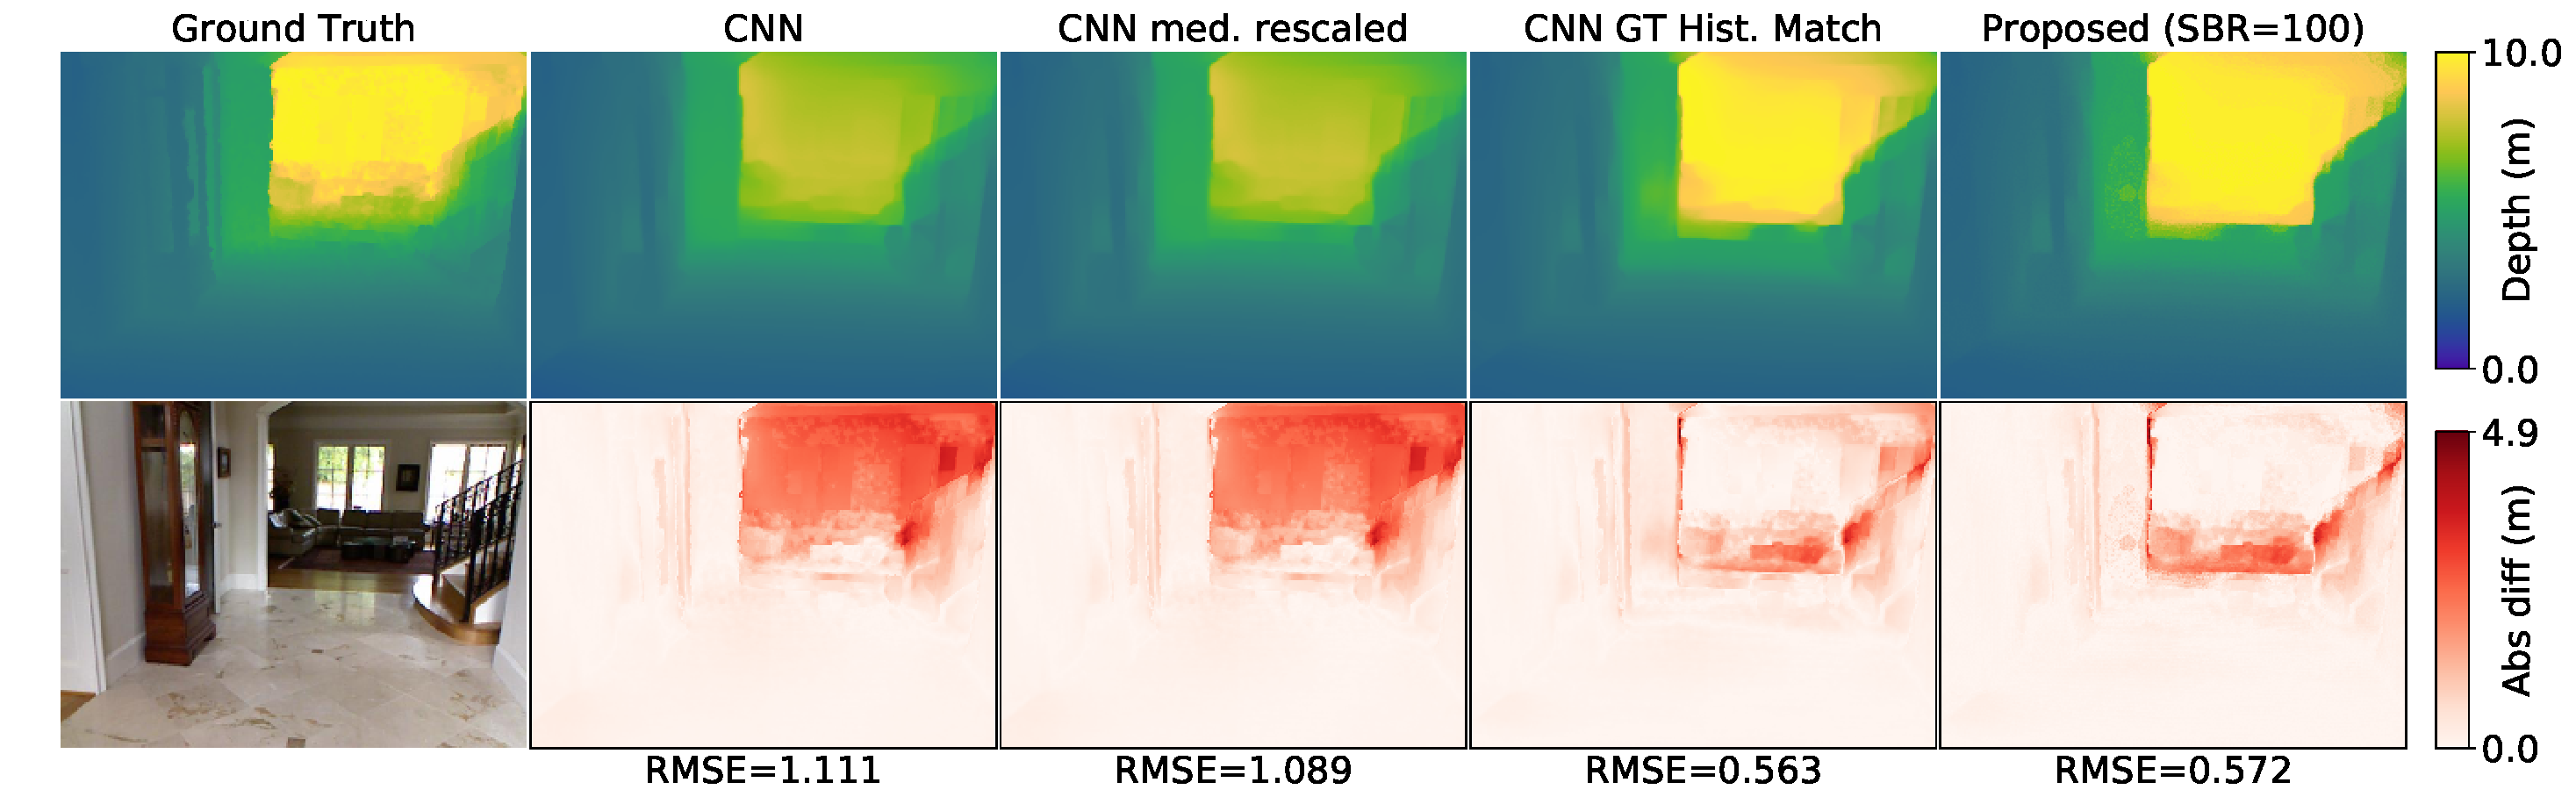
\includegraphics[width=\textwidth]{comparison/densedepth_140_comparison.pdf}
%   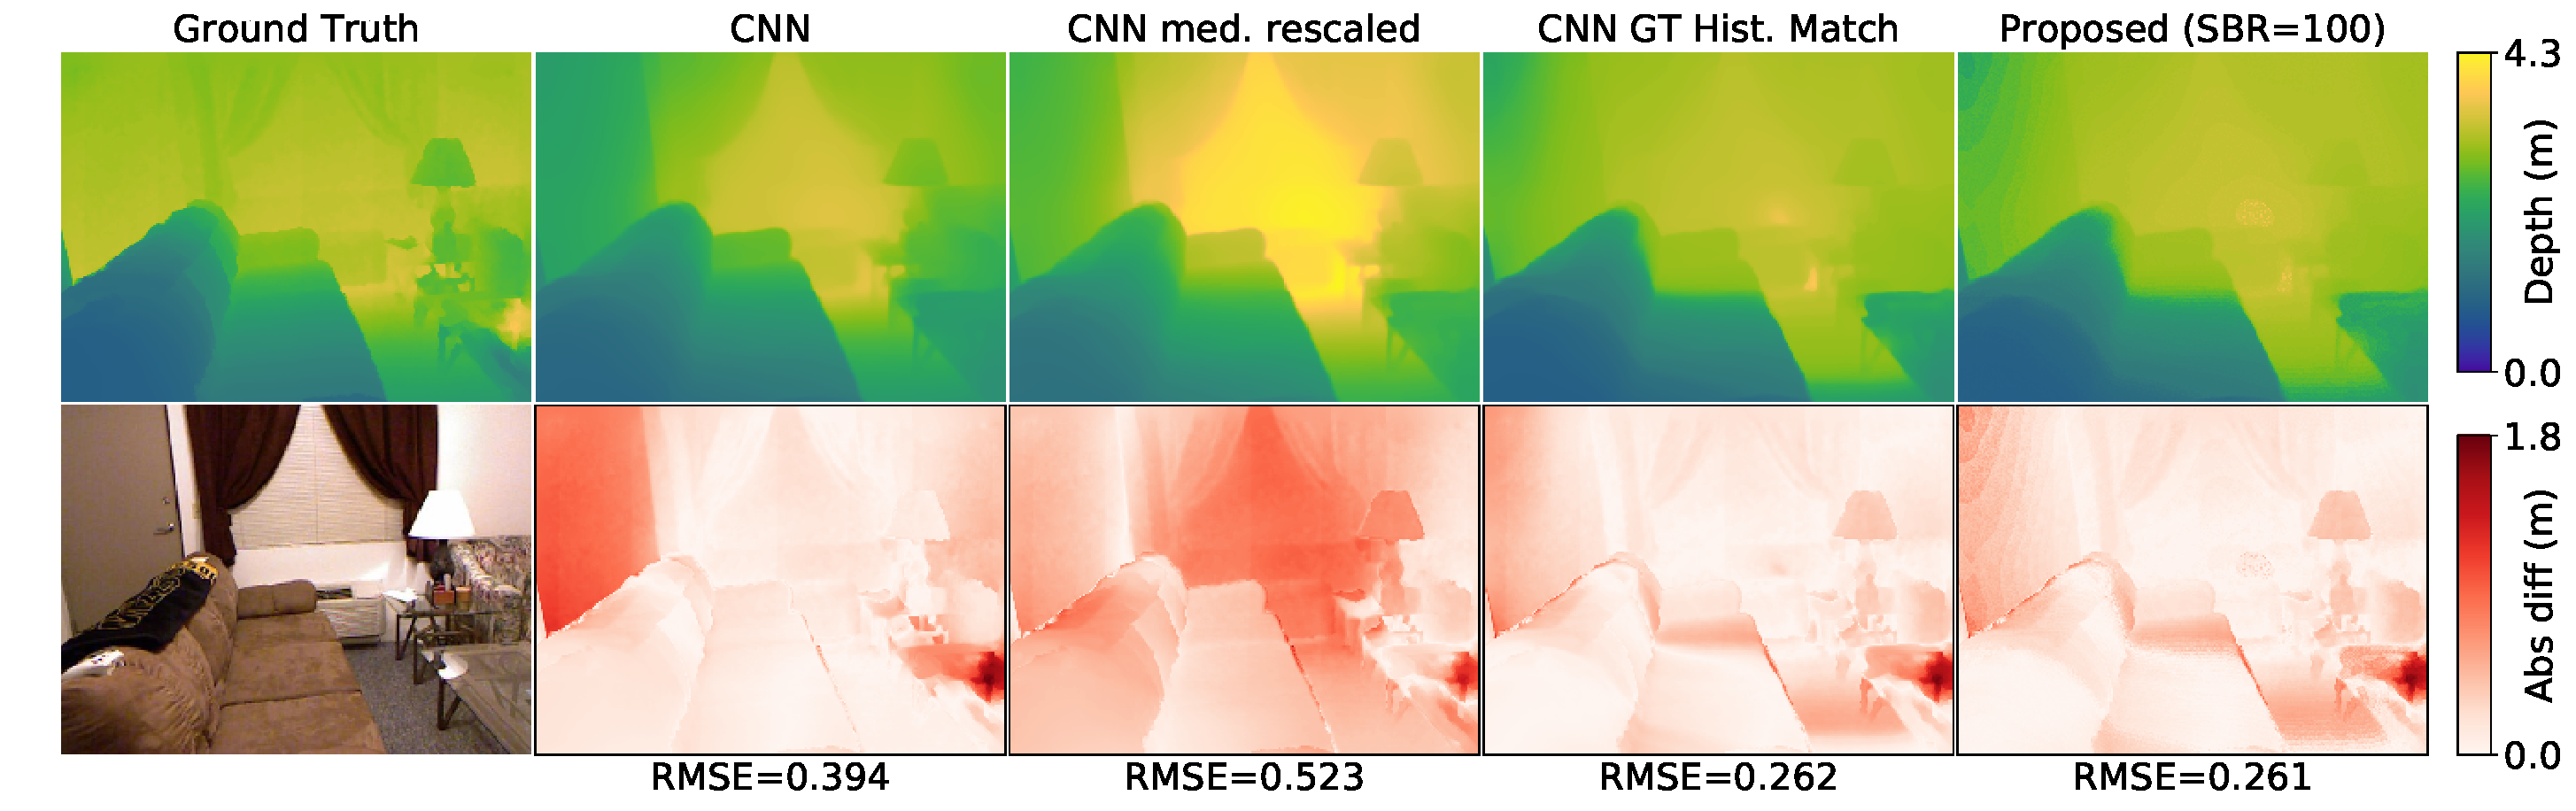
\includegraphics[width=\textwidth]{comparison/densedepth_244_comparison.pdf}
%   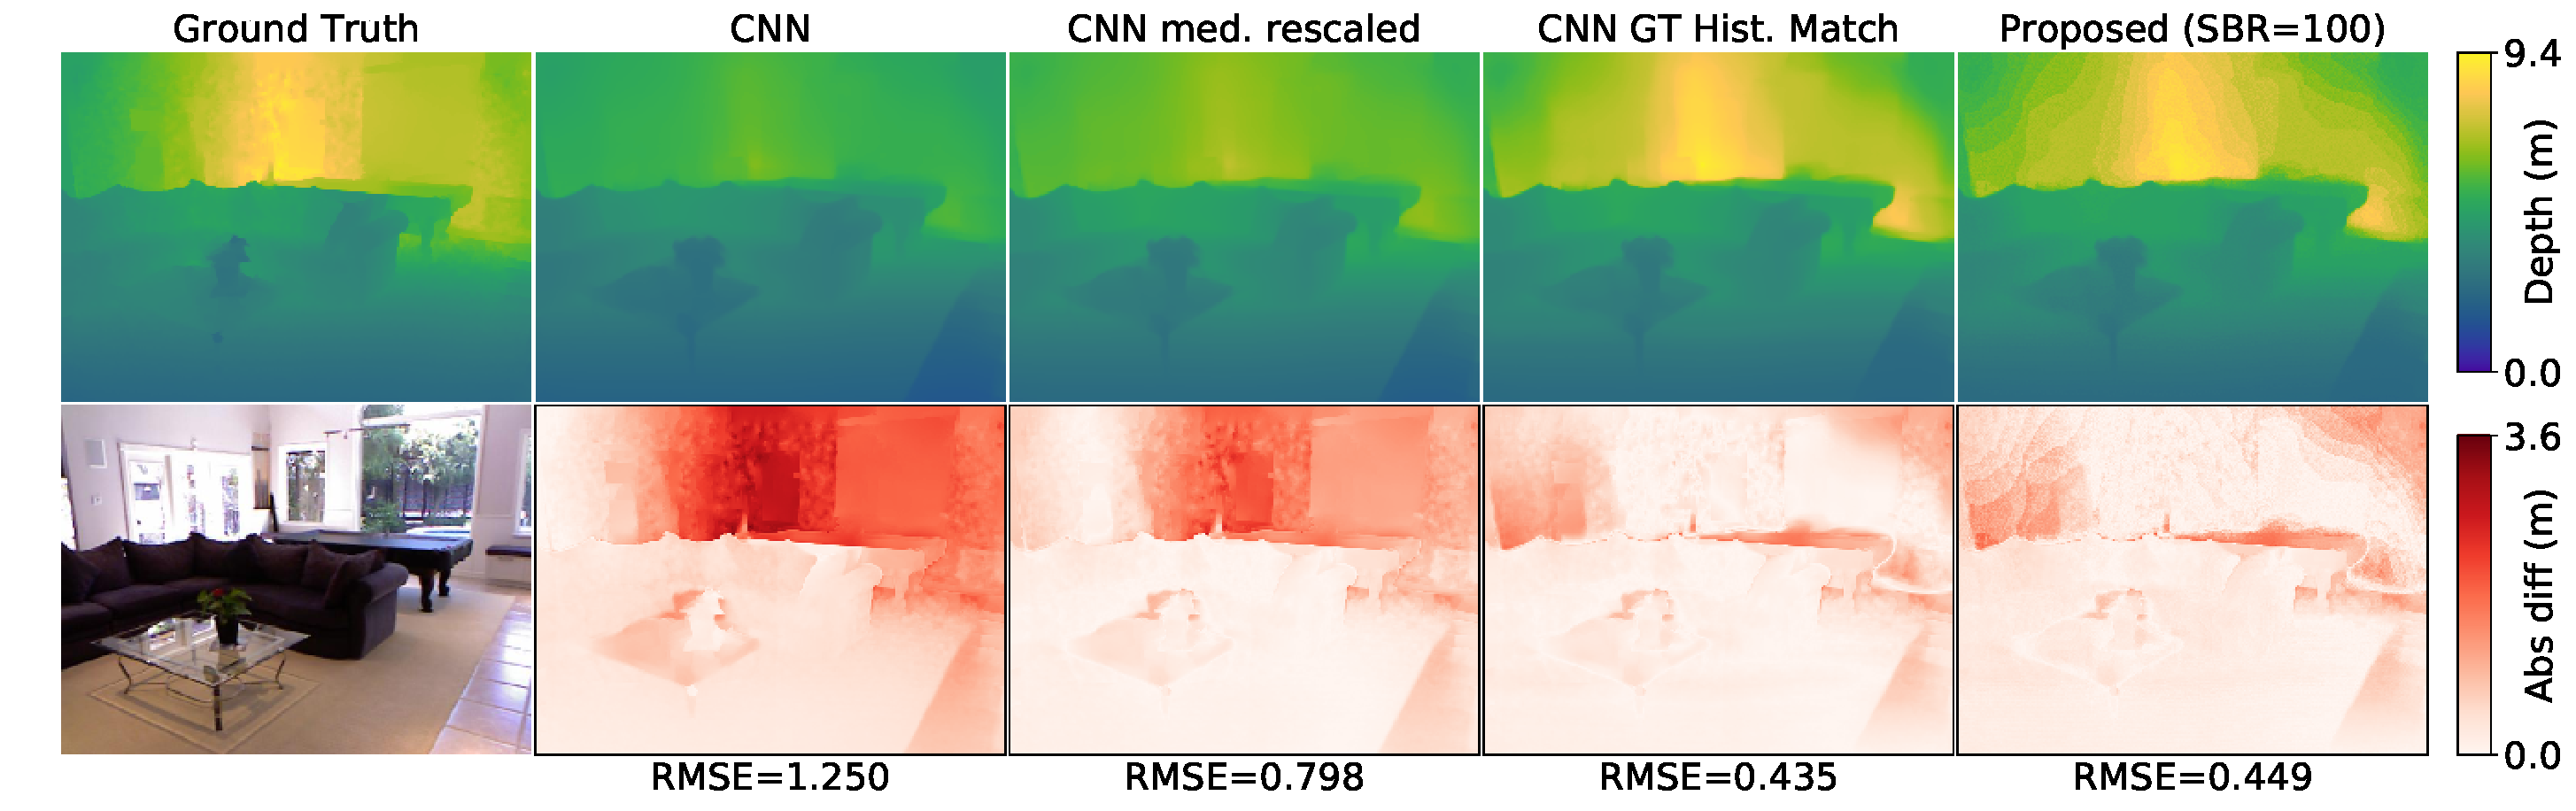
\includegraphics[width=\textwidth]{comparison/densedepth_527_comparison.pdf}
%   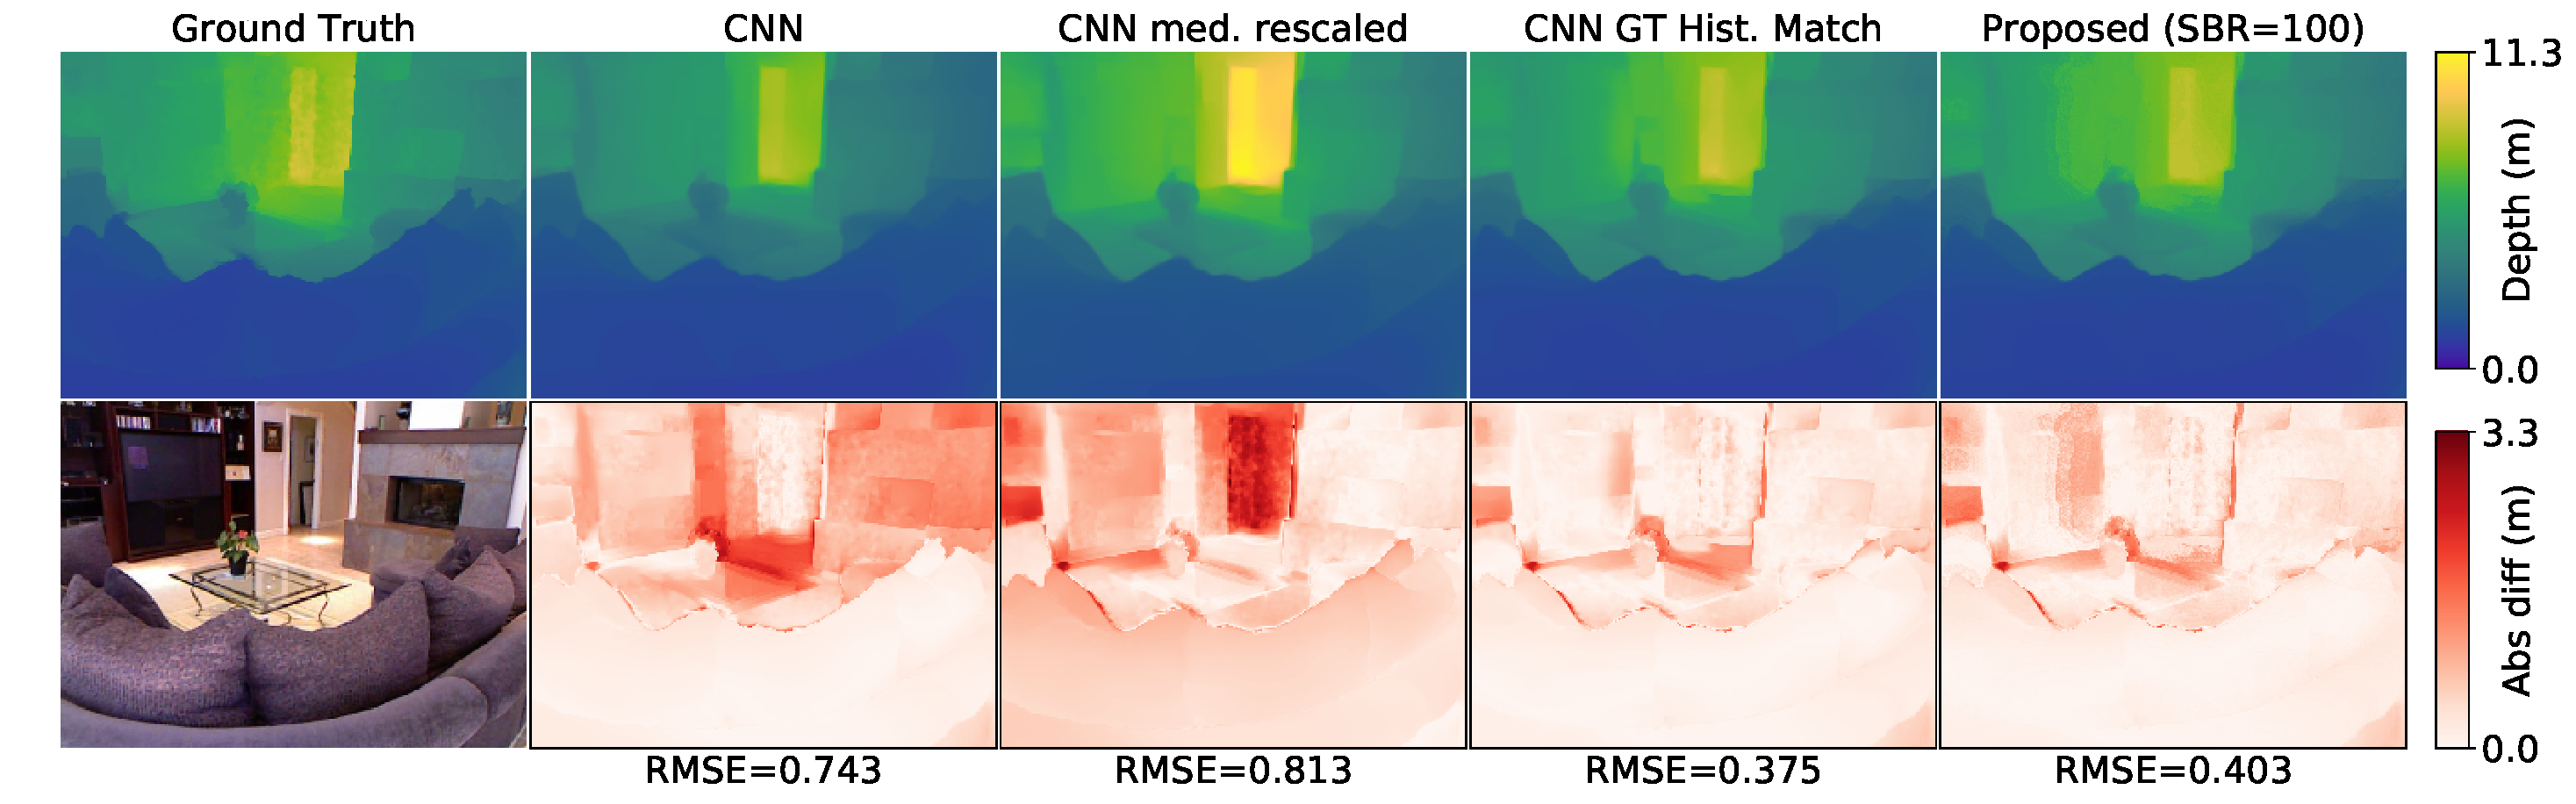
\includegraphics[width=\textwidth]{comparison/densedepth_529_comparison.pdf}
%   \caption{Results on DenseDepth}
% \end{figure}
% \begin{figure}
%   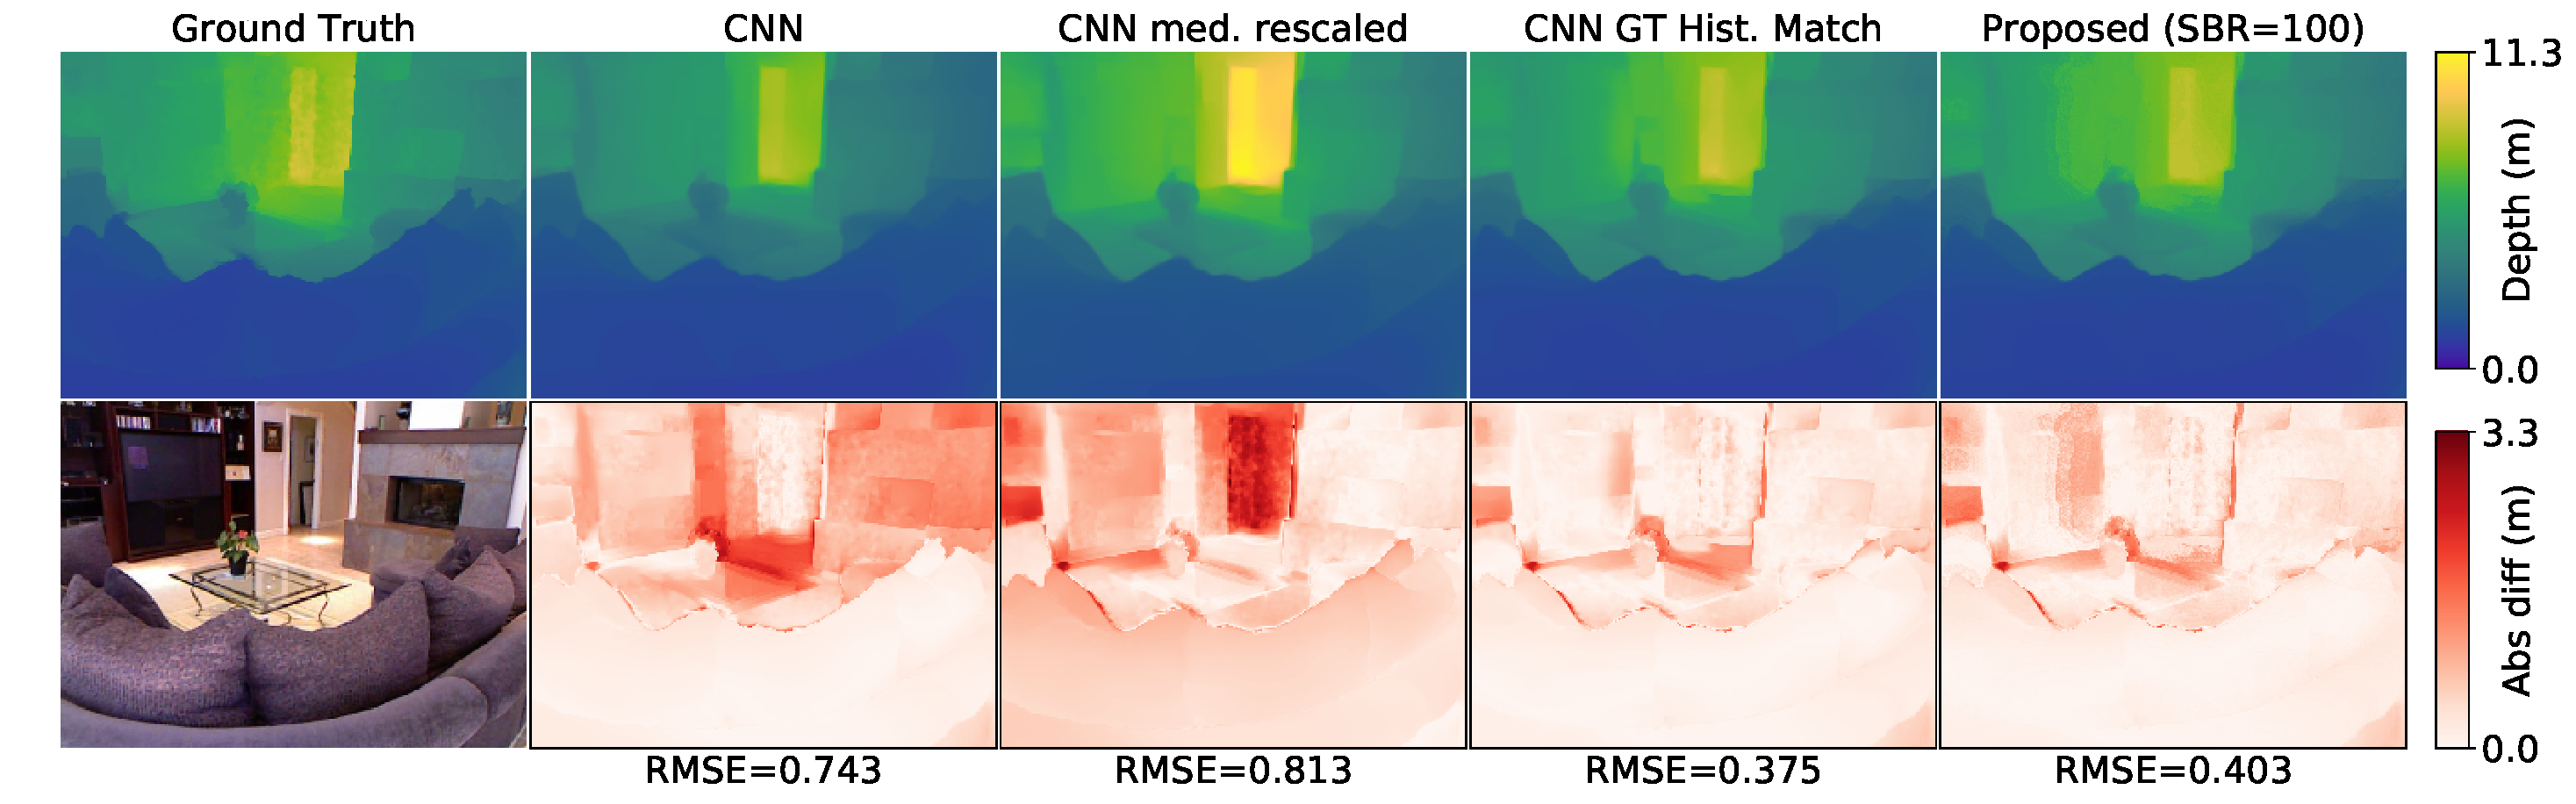
\includegraphics[width=\textwidth]{comparison/densedepth_529_comparison.pdf}
%   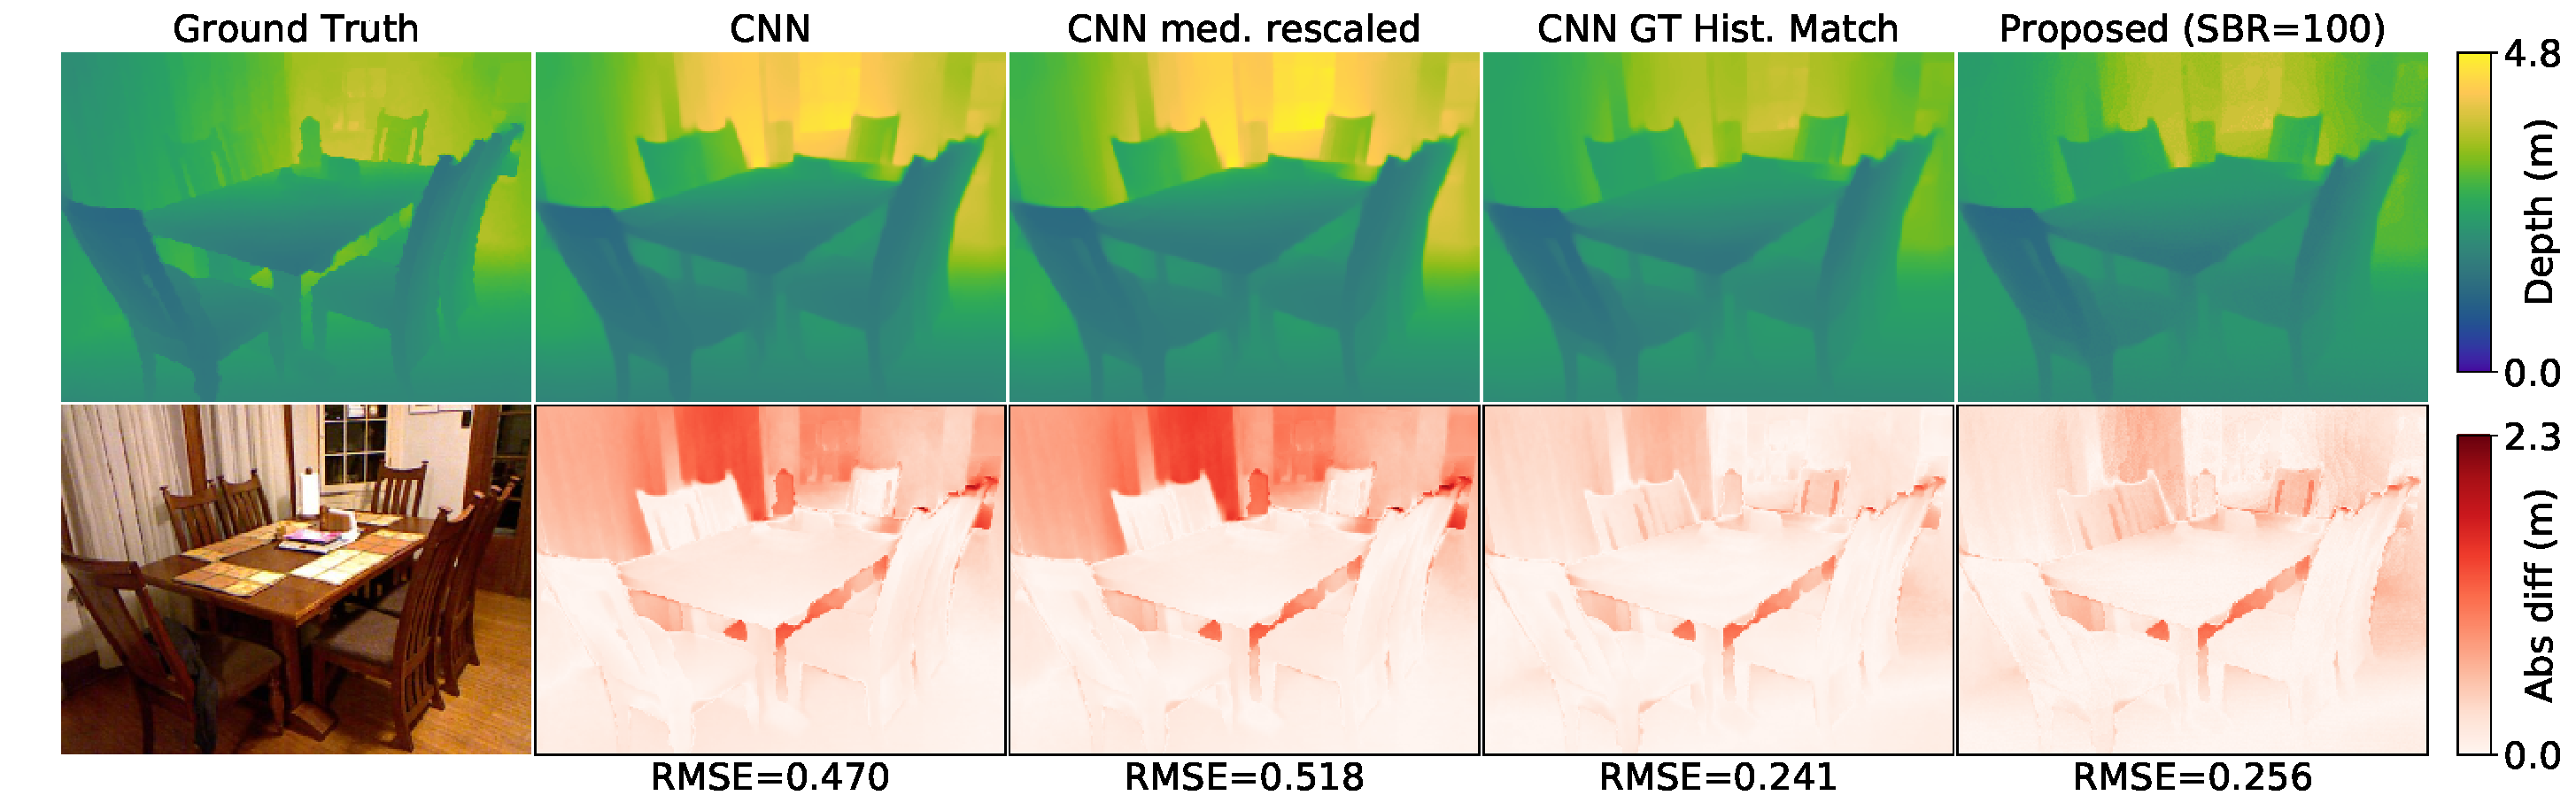
\includegraphics[width=\textwidth]{comparison/densedepth_219_comparison.pdf}
%   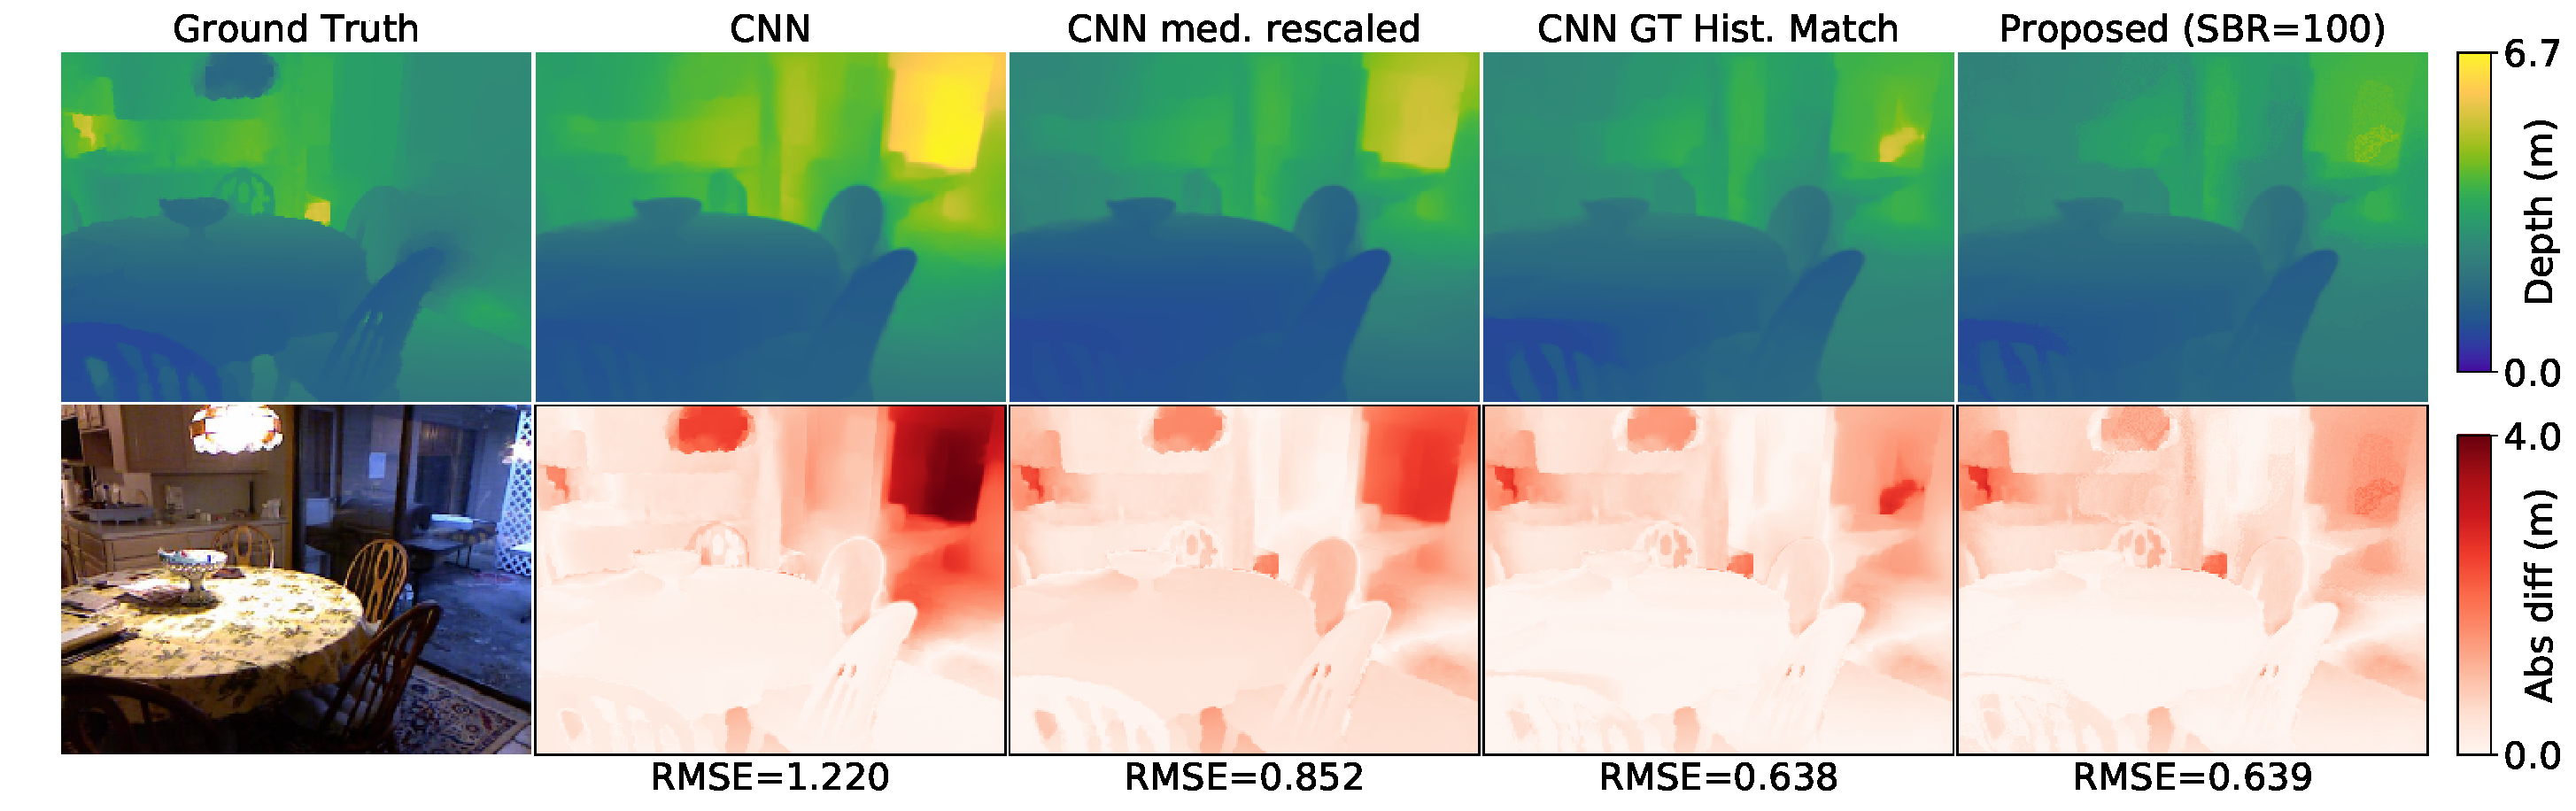
\includegraphics[width=\textwidth]{comparison/densedepth_329_comparison.pdf}
%   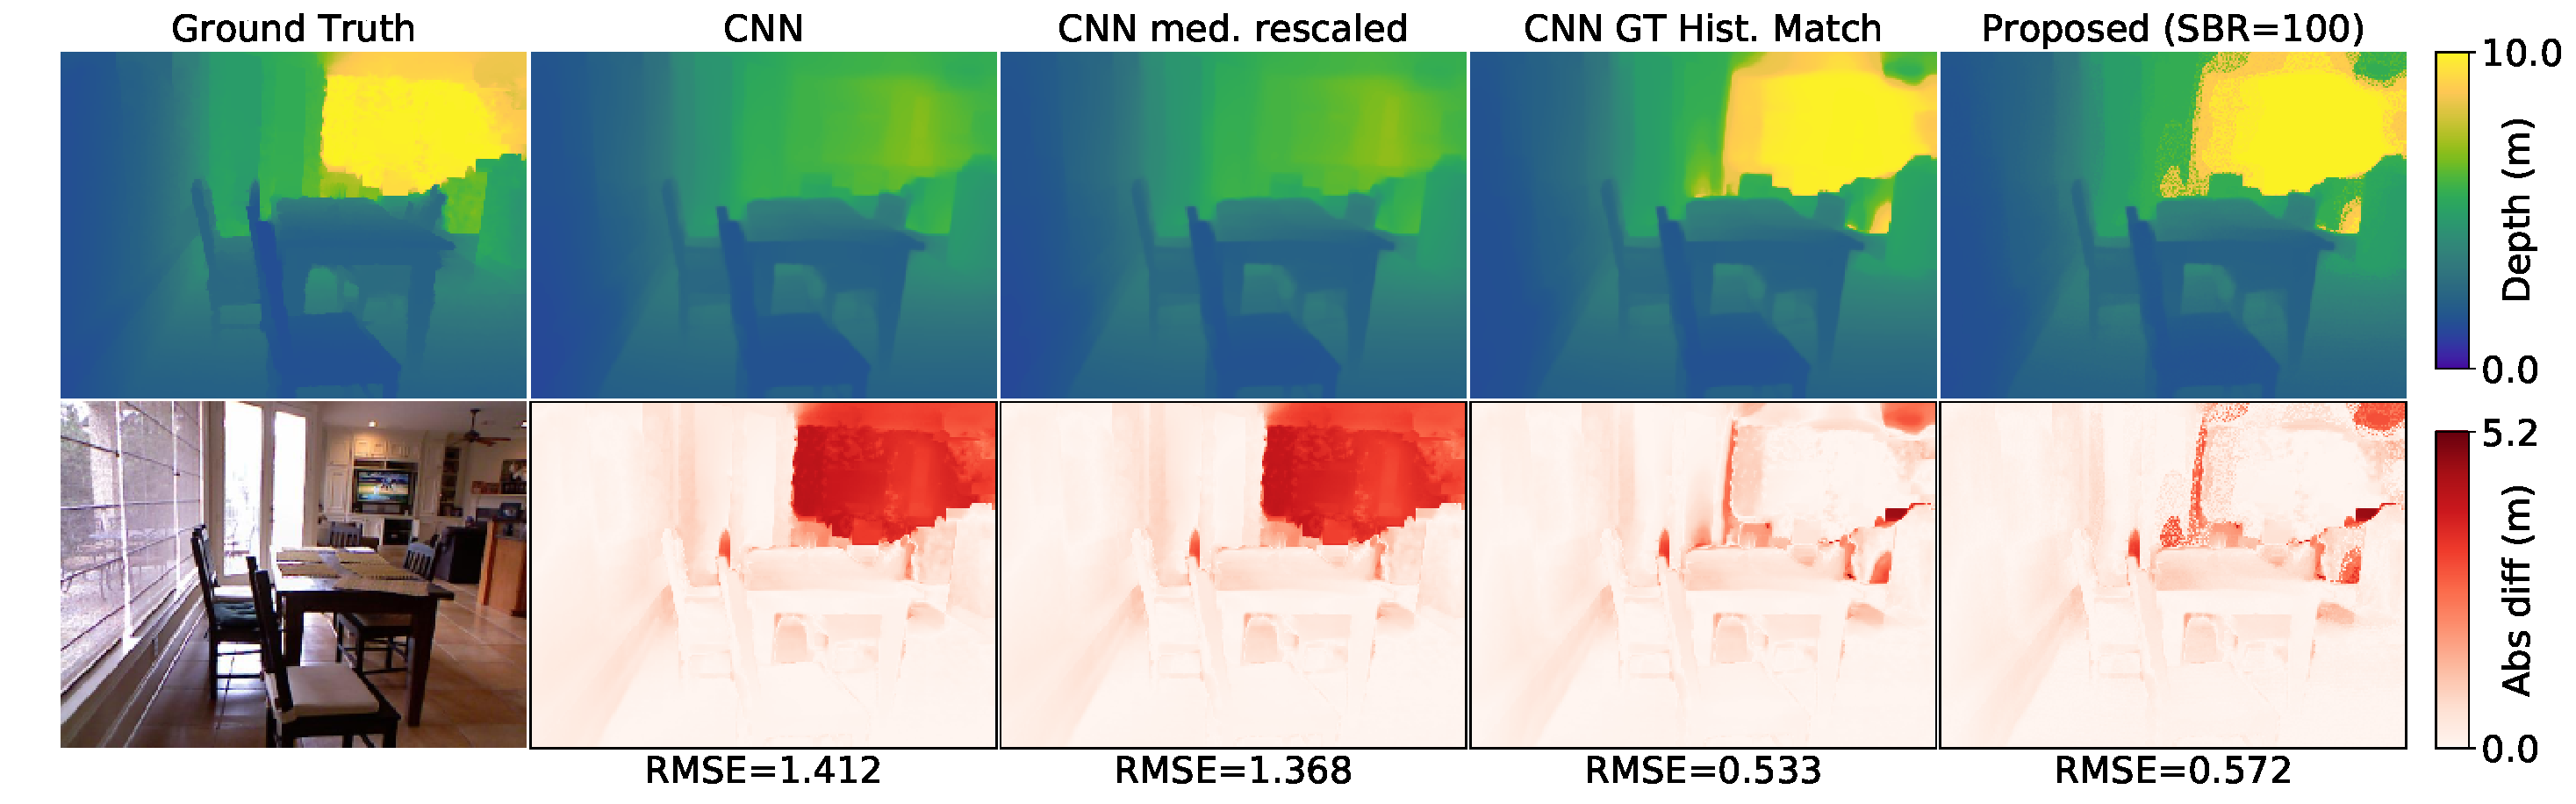
\includegraphics[width=\textwidth]{comparison/densedepth_346_comparison.pdf}
%   \caption{Results on DenseDepth}
% \end{figure}
% \begin{figure}
%   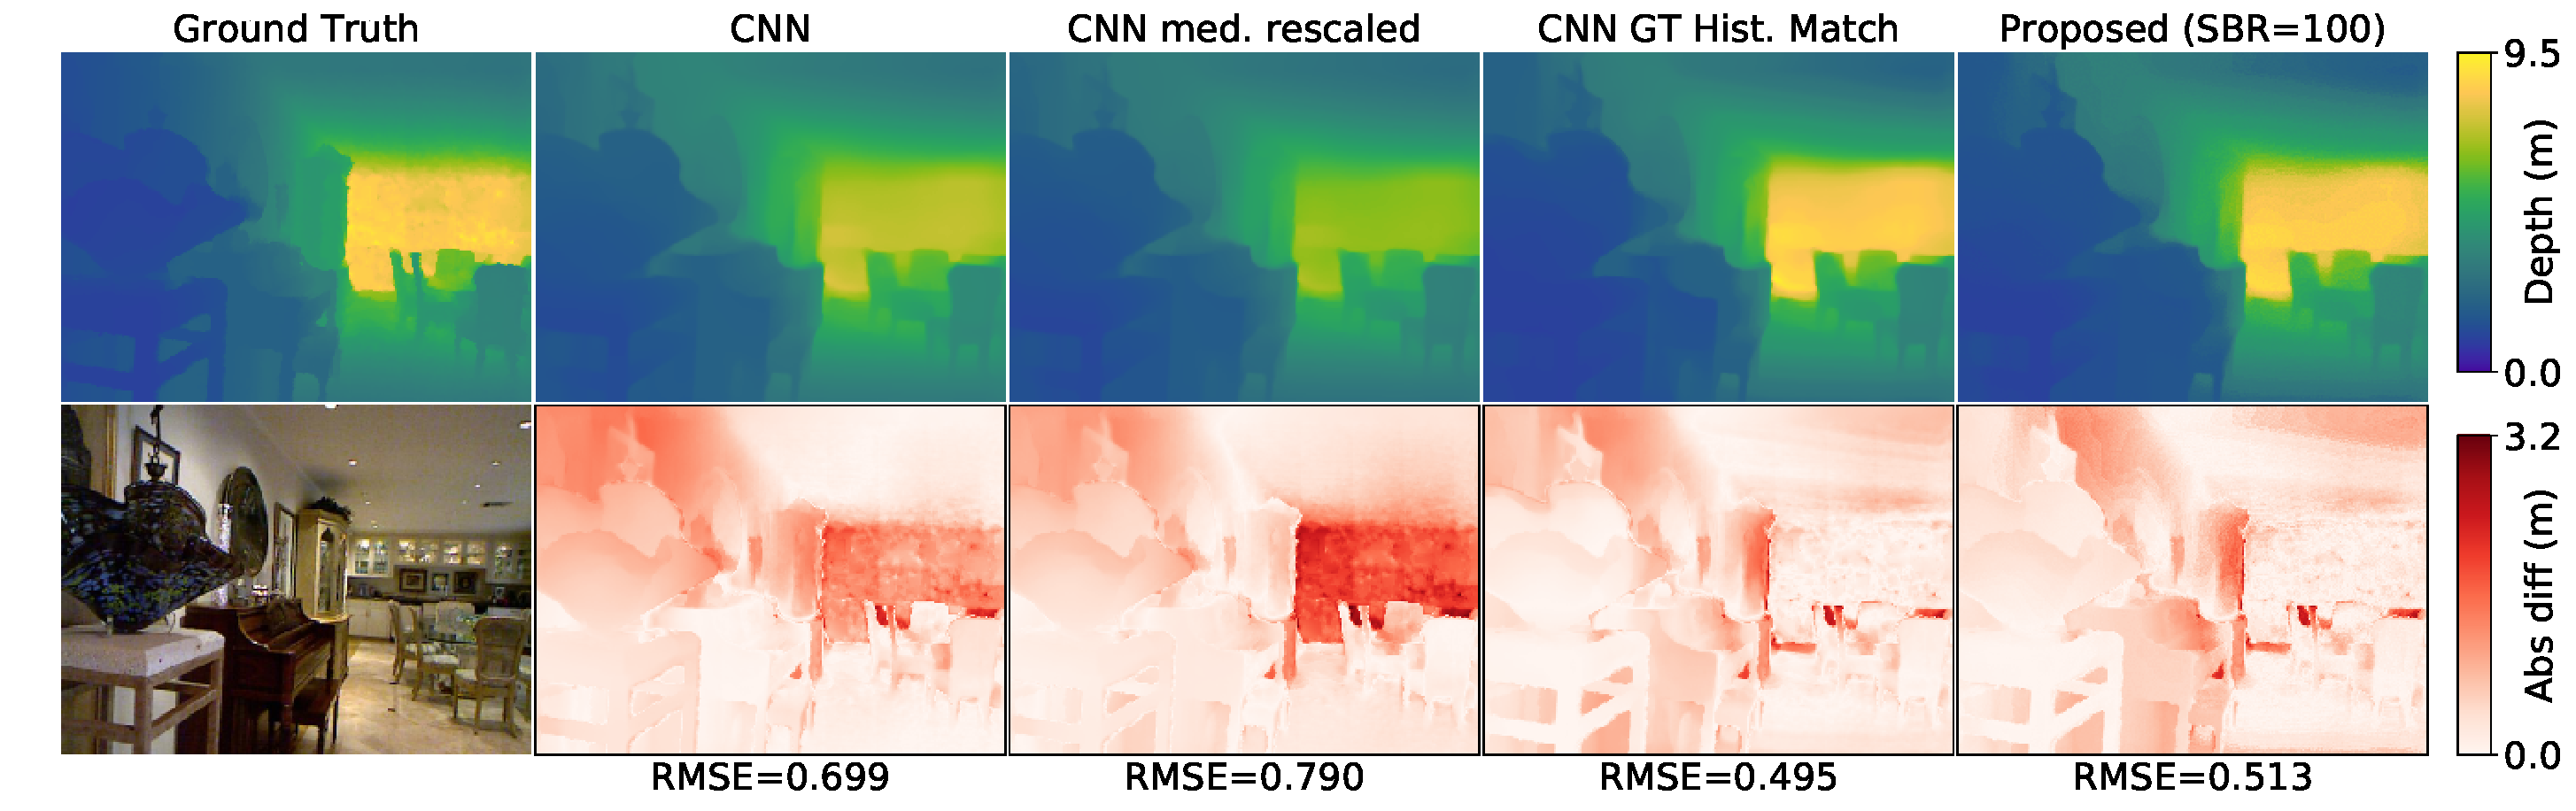
\includegraphics[width=\textwidth]{comparison/densedepth_616_comparison.pdf}
%   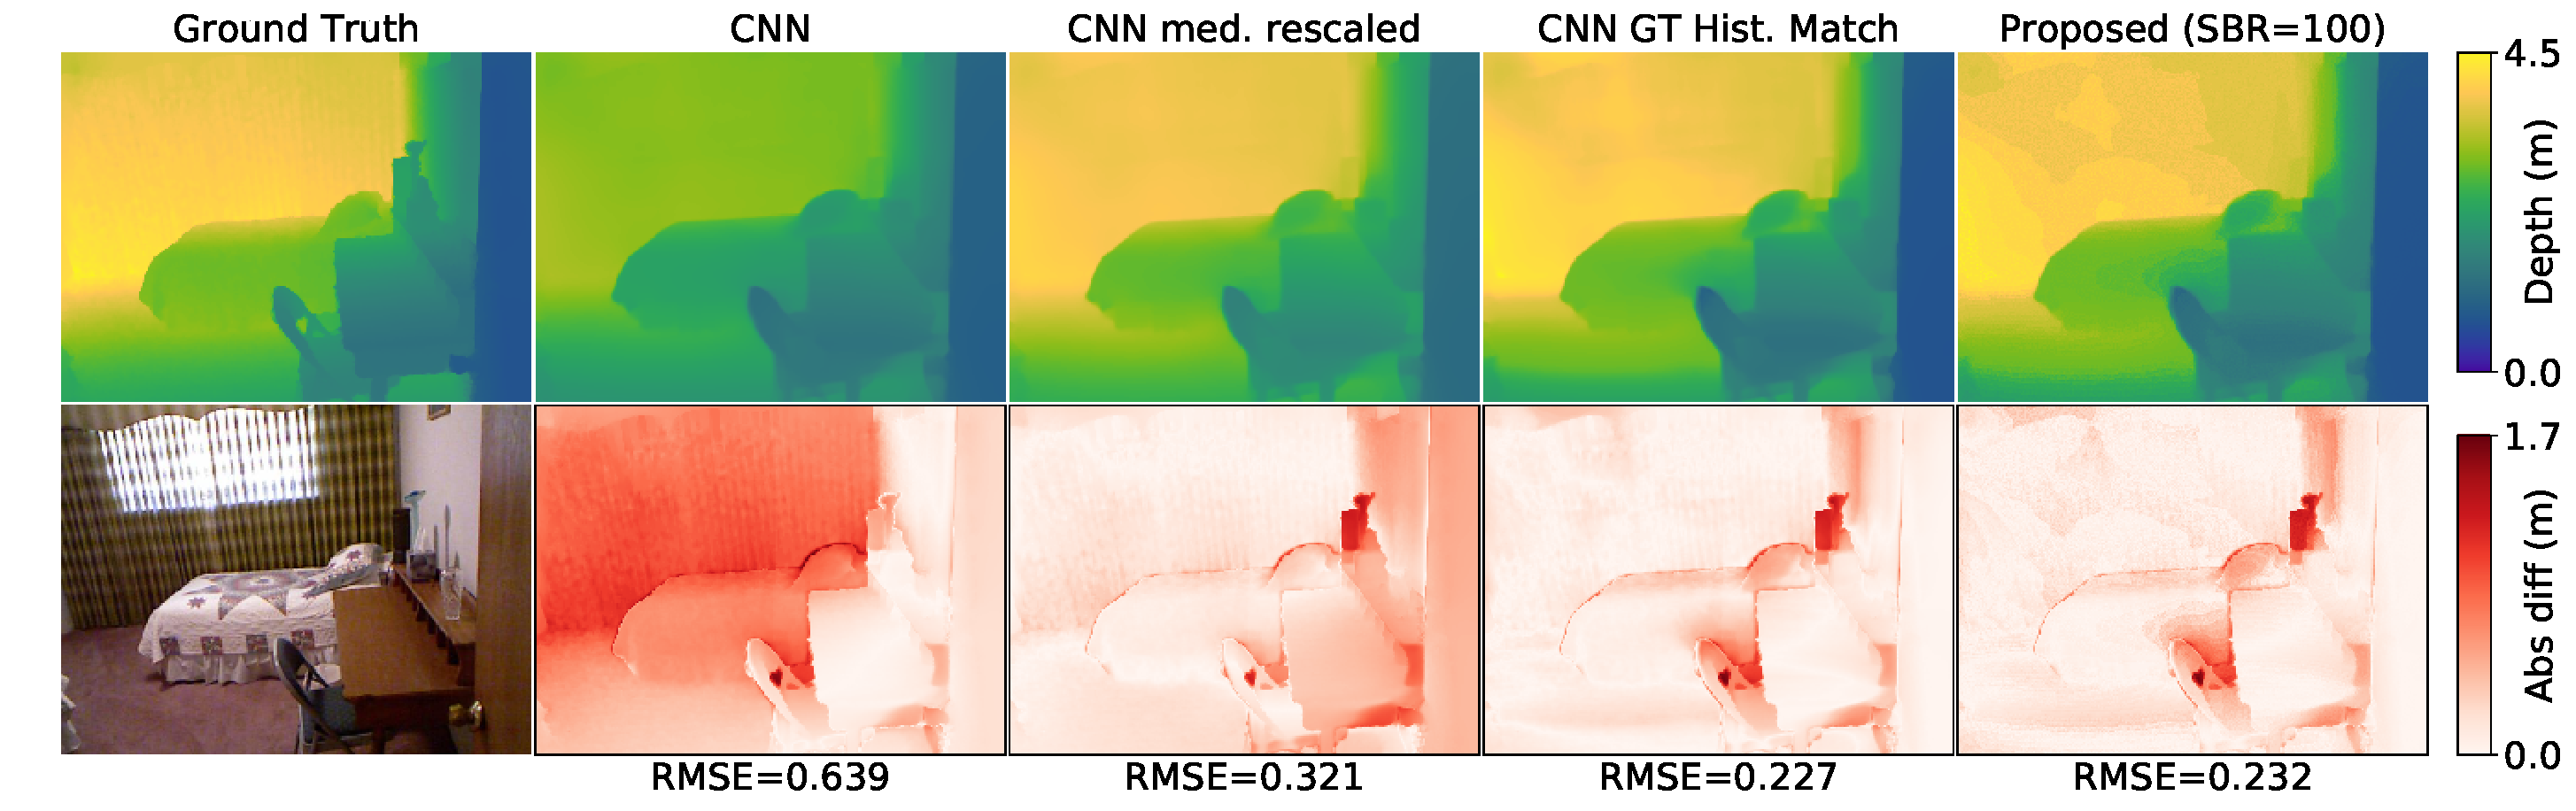
\includegraphics[width=\textwidth]{comparison/densedepth_390_comparison.pdf}
%   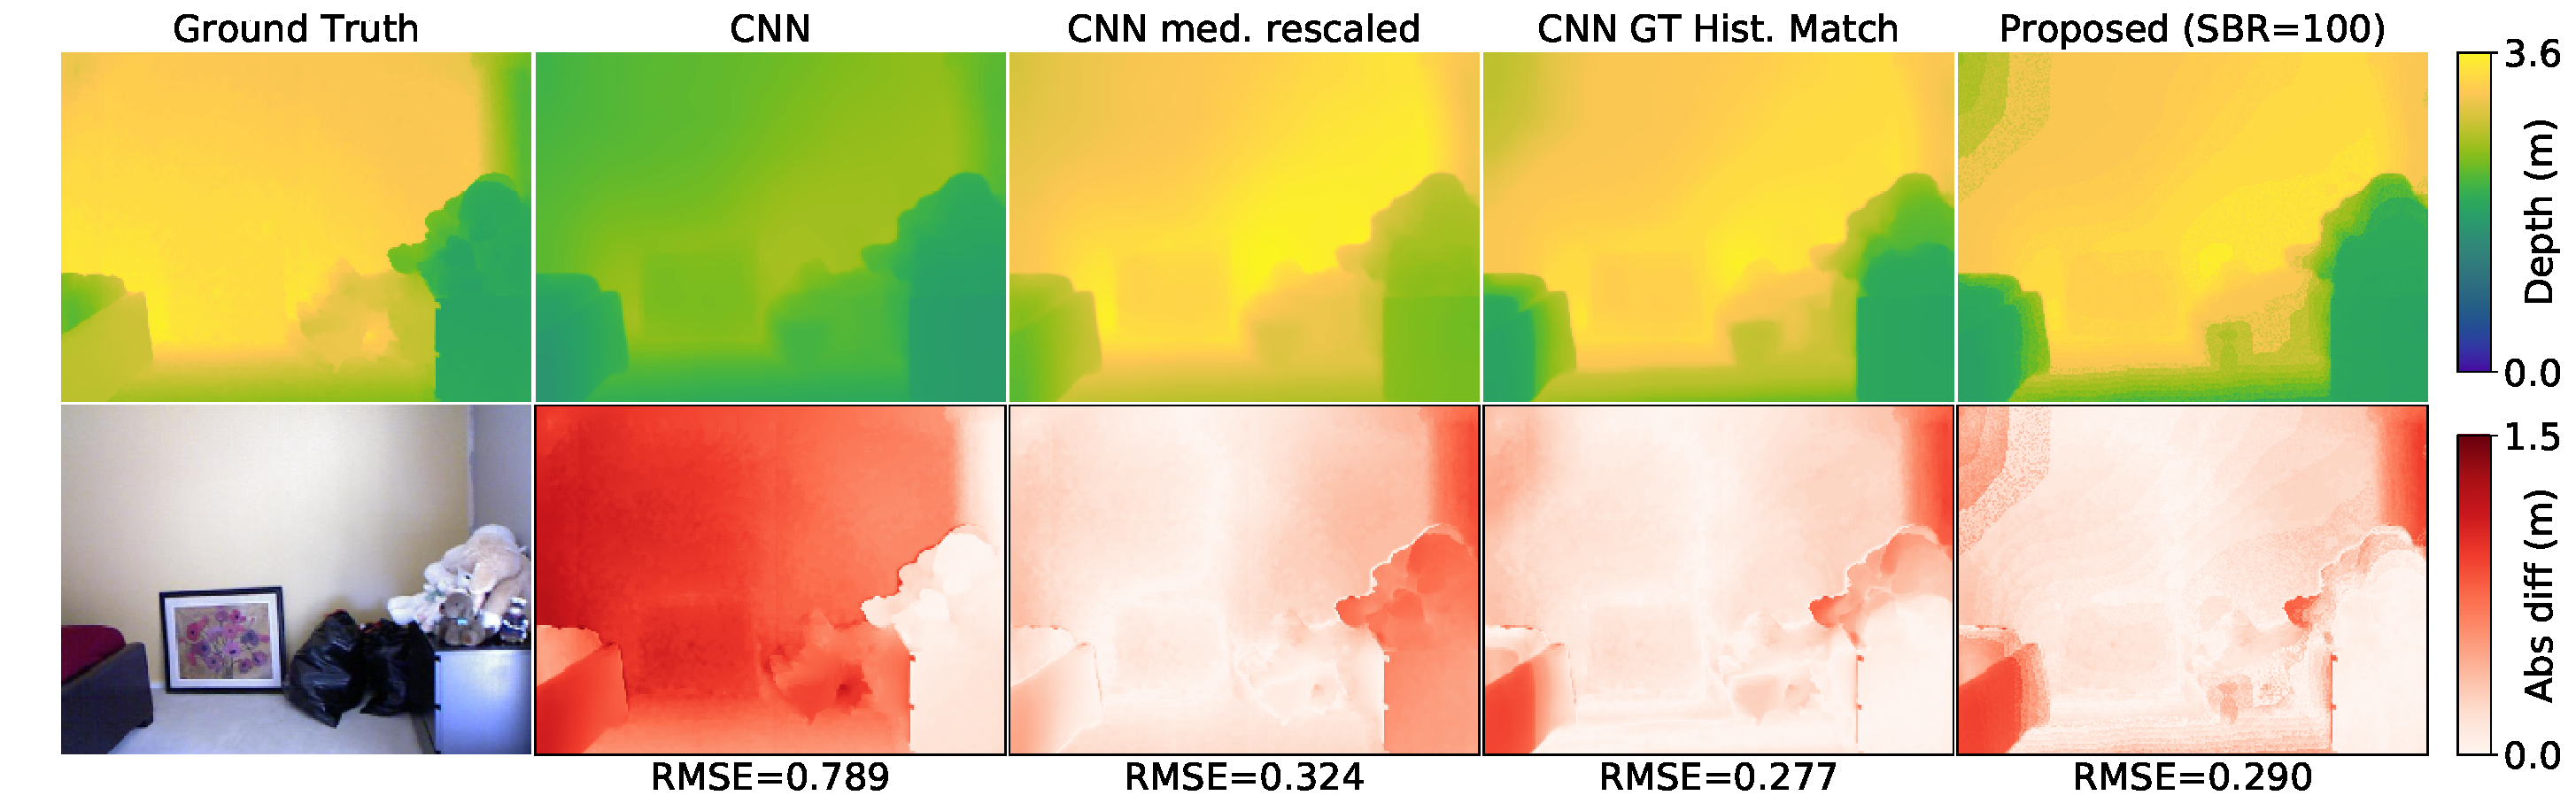
\includegraphics[width=\textwidth]{comparison/densedepth_412_comparison.pdf}
%   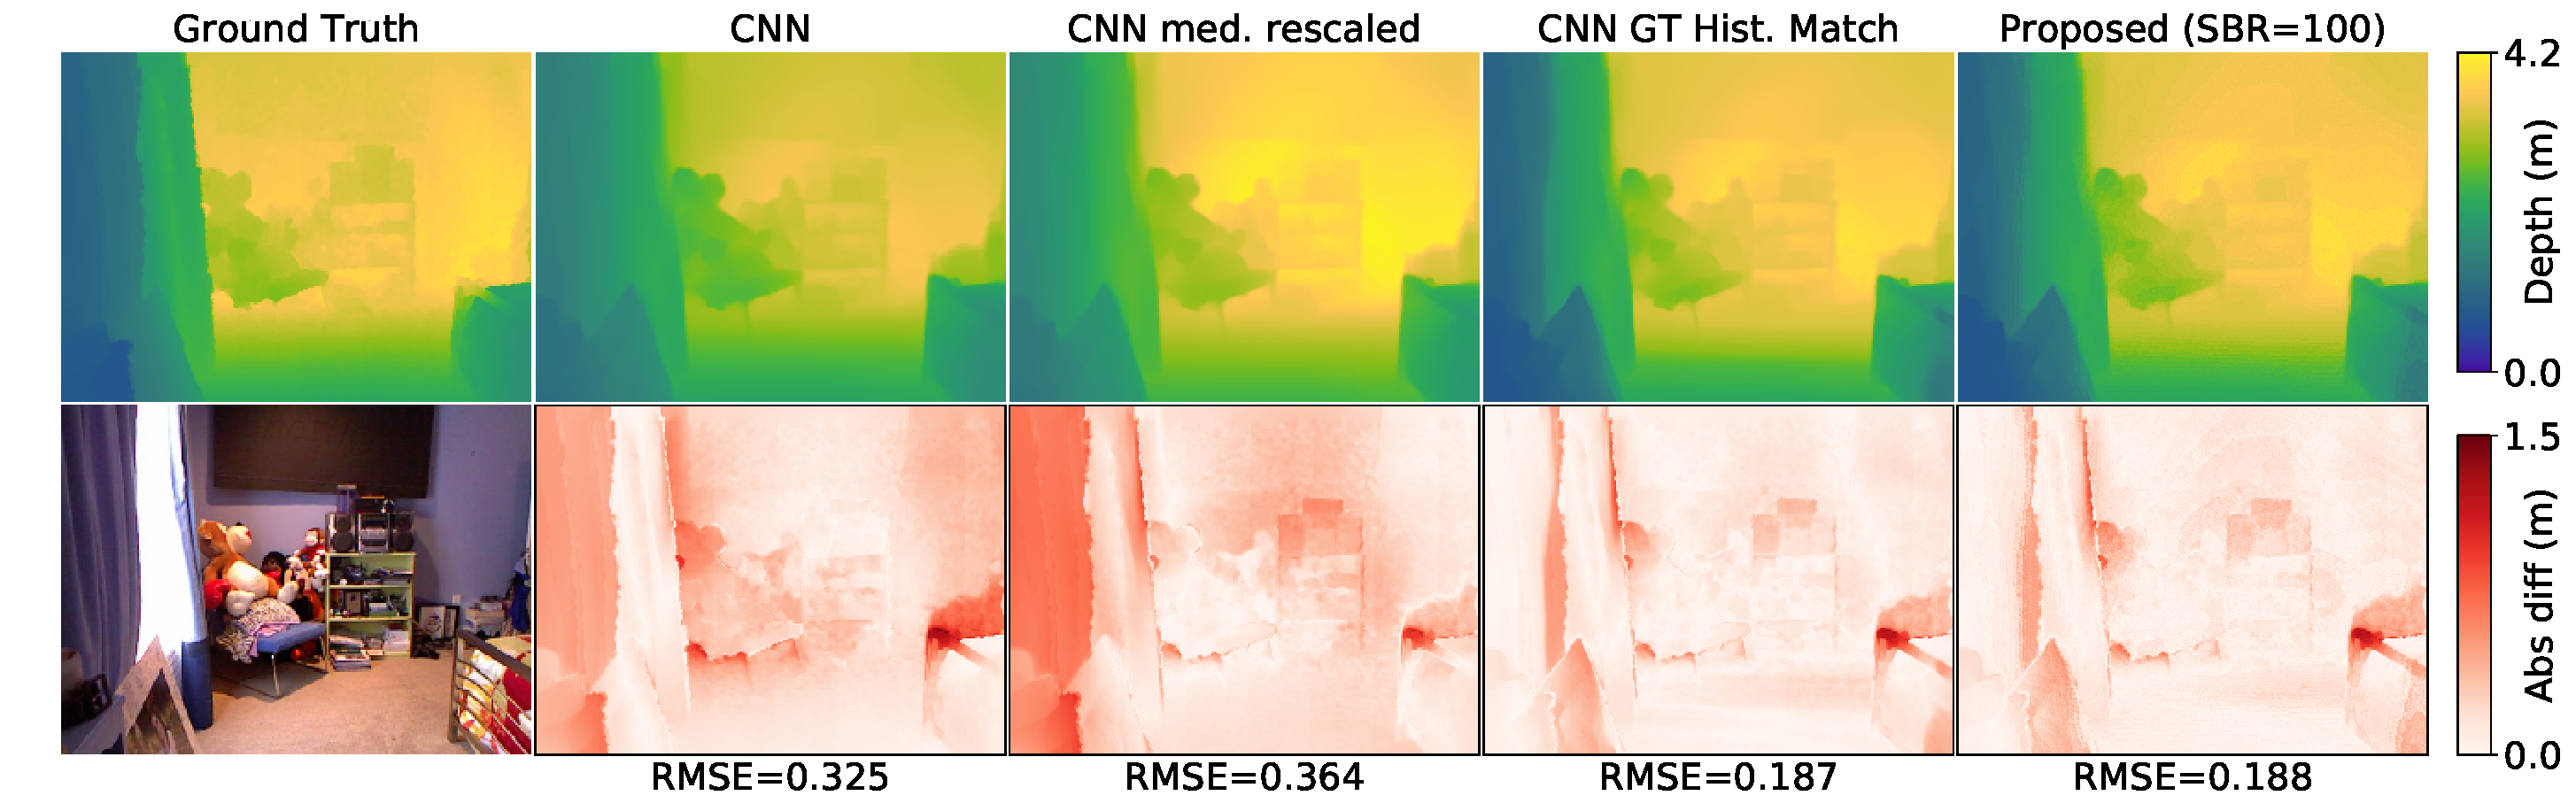
\includegraphics[width=\textwidth]{comparison/densedepth_420_comparison.pdf}
%   \caption{Results on DenseDepth}
% \end{figure}
% \begin{figure}
%   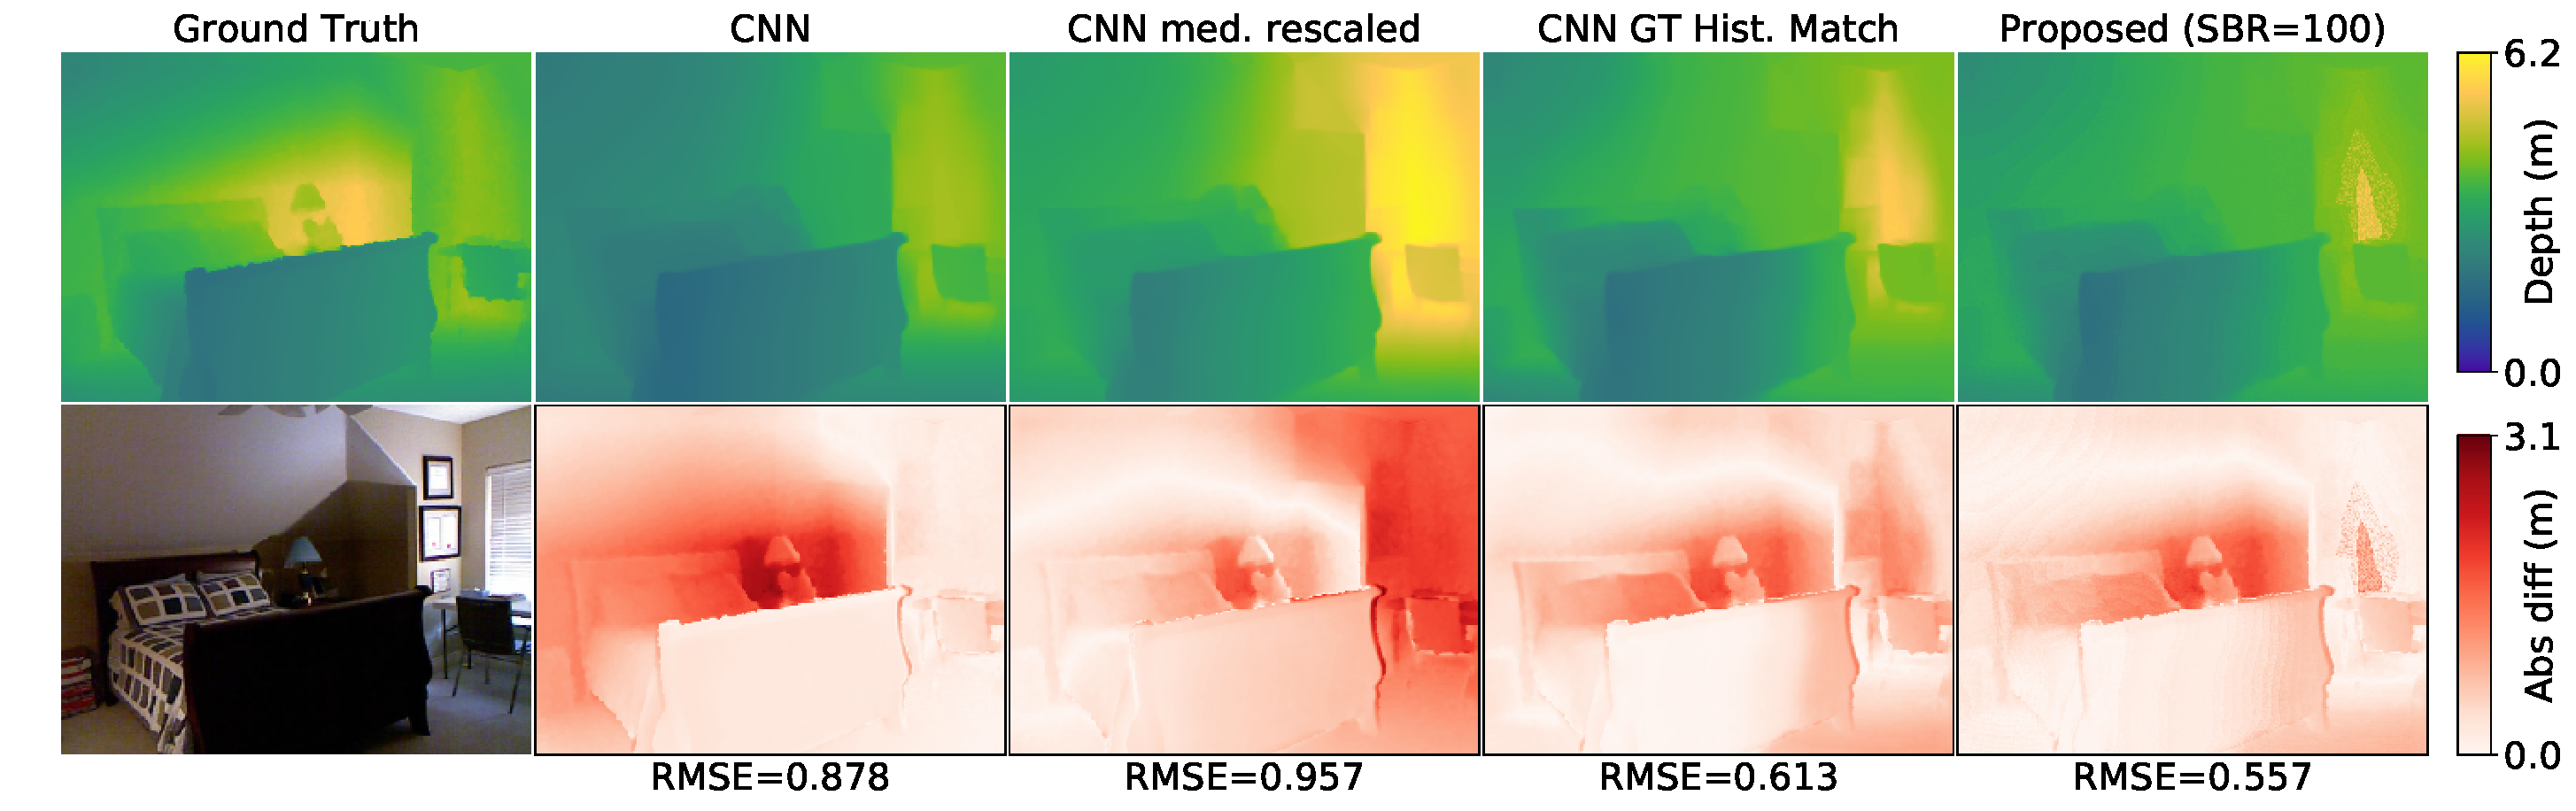
\includegraphics[width=\textwidth]{comparison/densedepth_428_comparison.pdf}
%   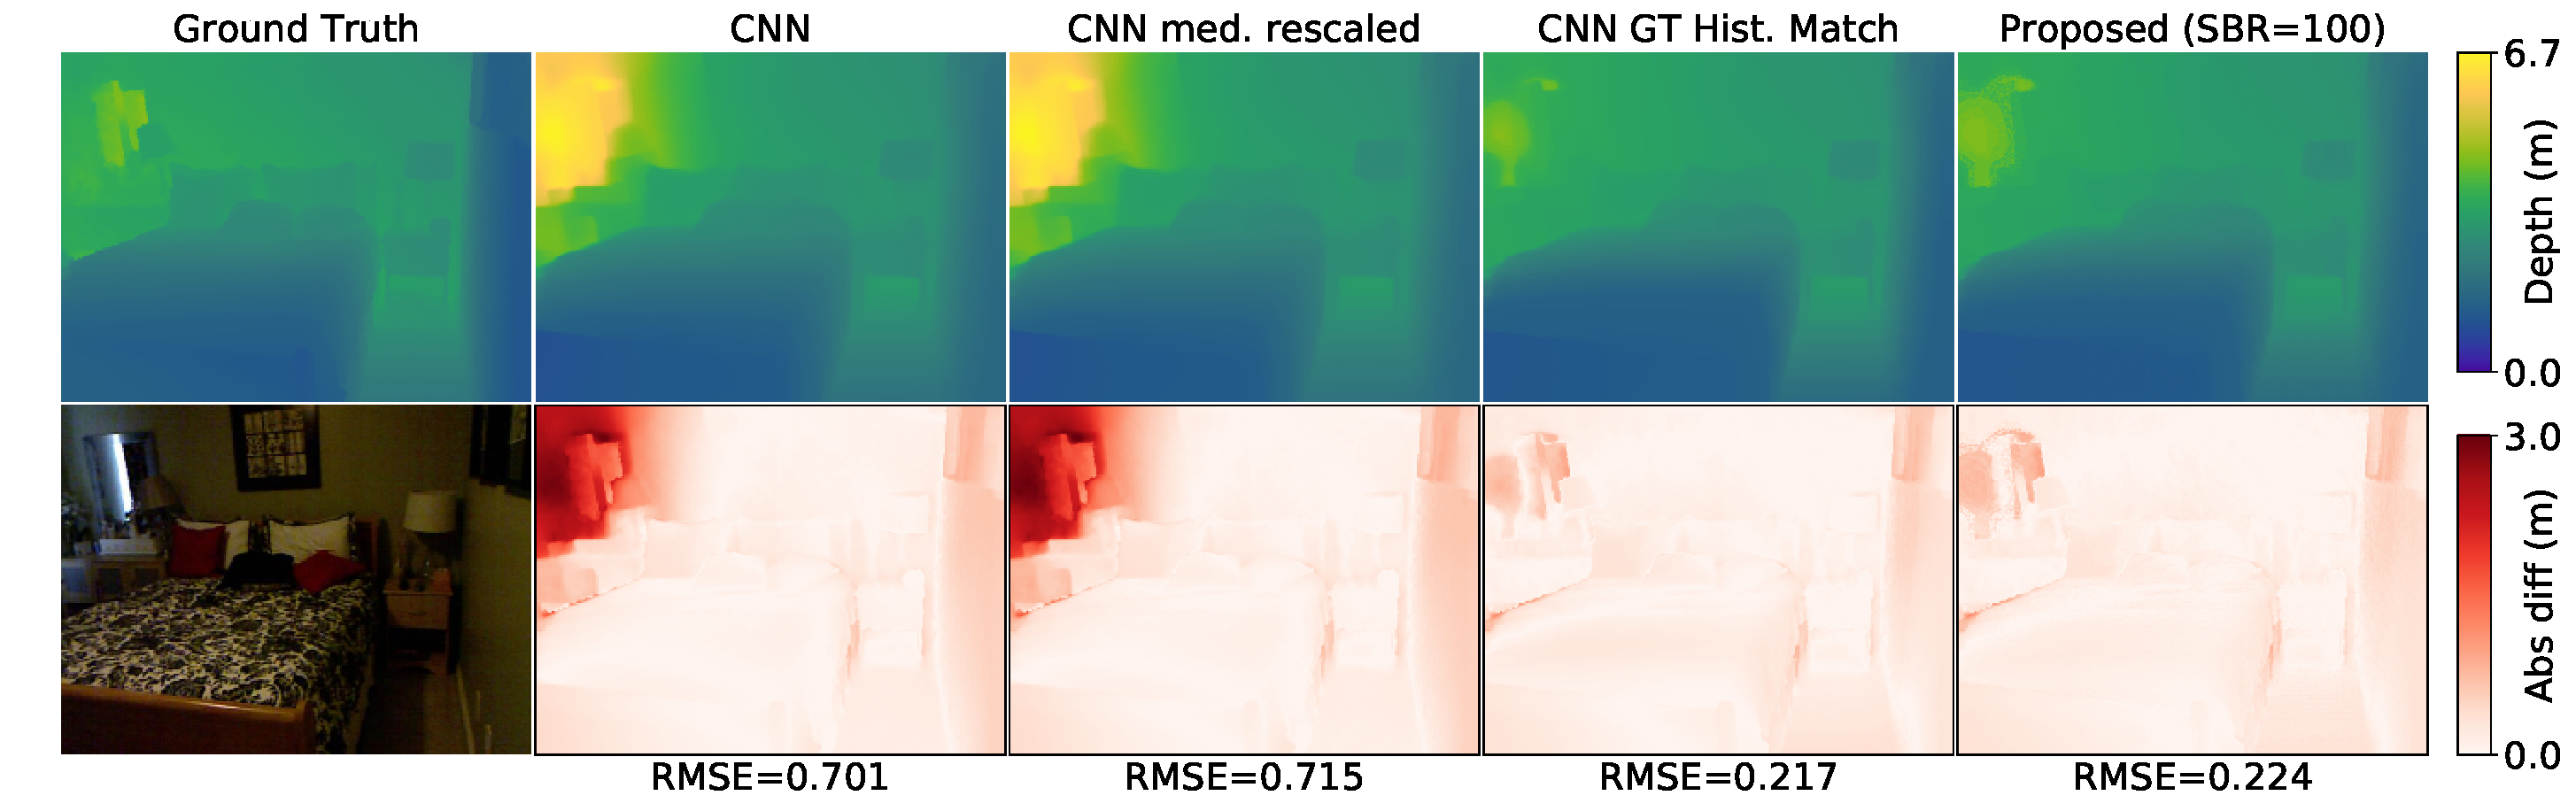
\includegraphics[width=\textwidth]{comparison/densedepth_457_comparison.pdf}
%   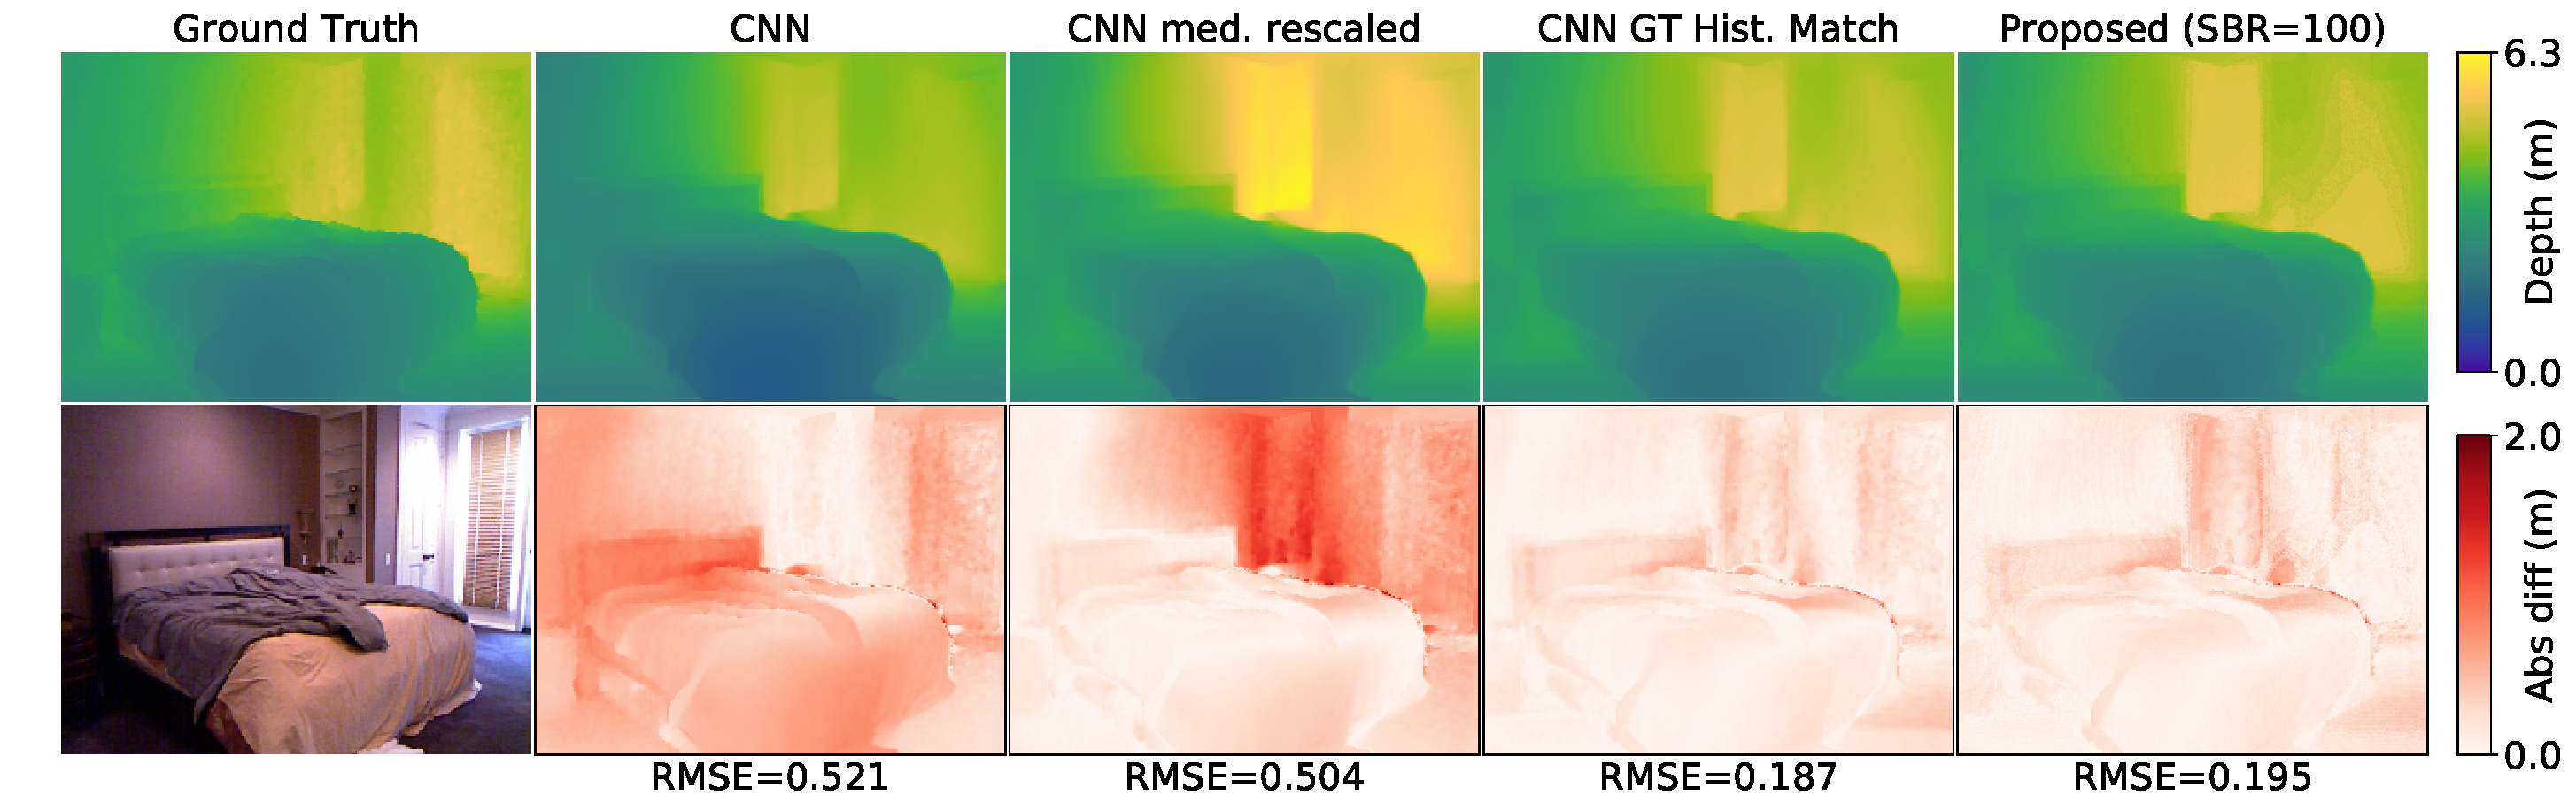
\includegraphics[width=\textwidth]{comparison/densedepth_468_comparison.pdf}
%   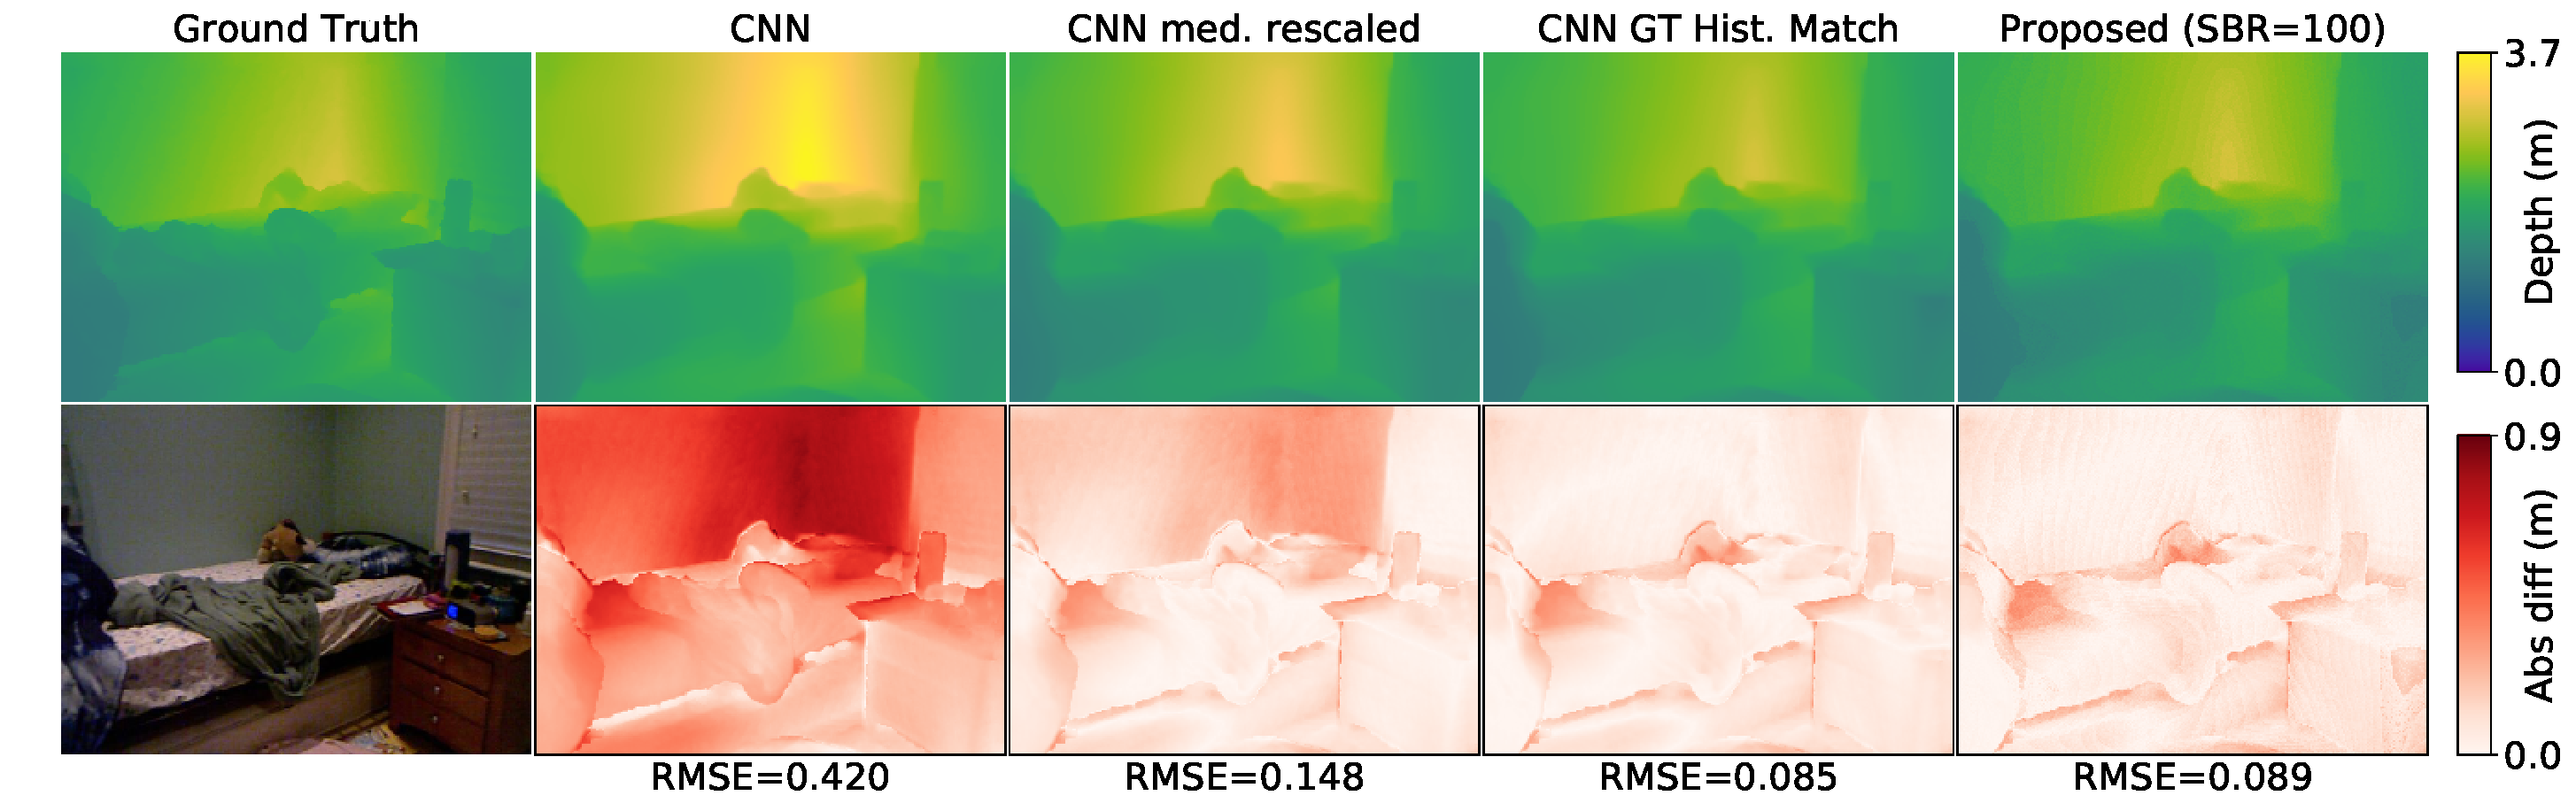
\includegraphics[width=\textwidth]{comparison/densedepth_477_comparison.pdf}
%   \caption{Results on DenseDepth}
% \end{figure}
%   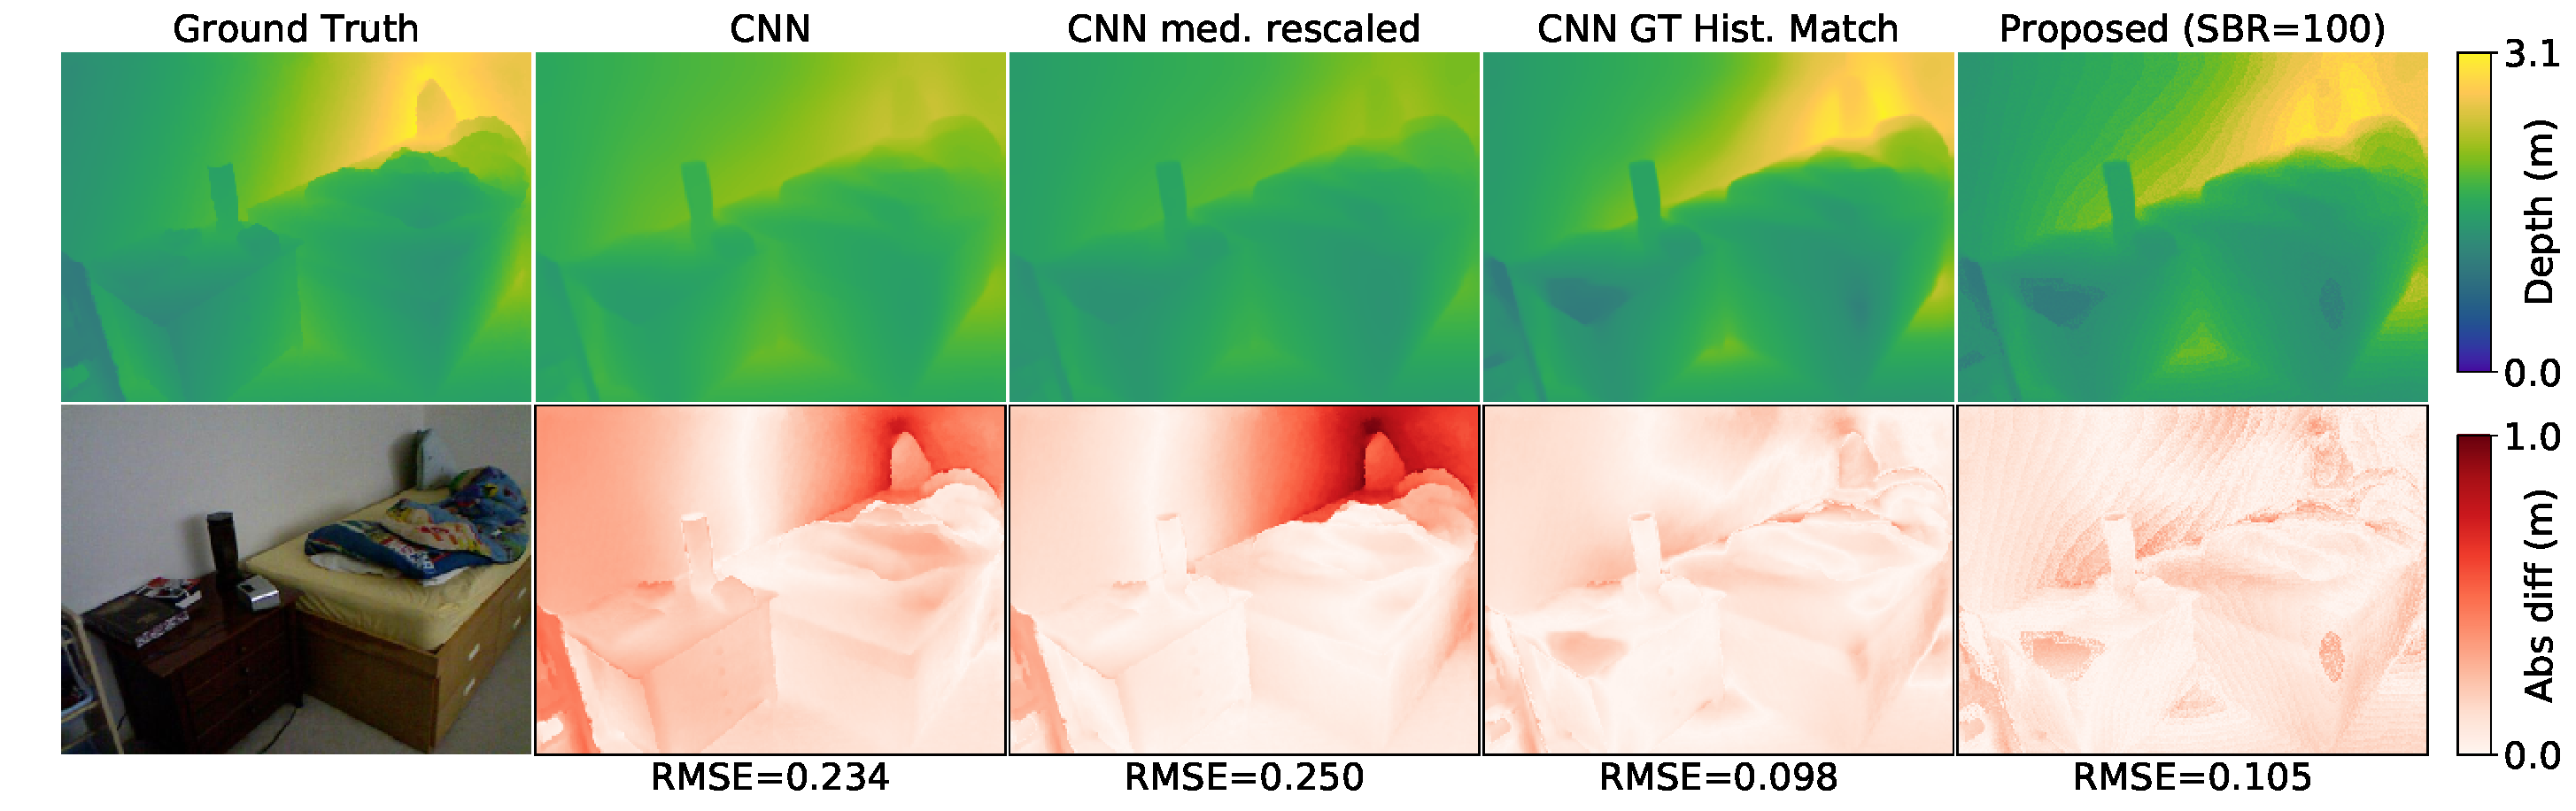
\includegraphics[height=3cm]{comparison/densedepth_499_comparison.pdf}
%   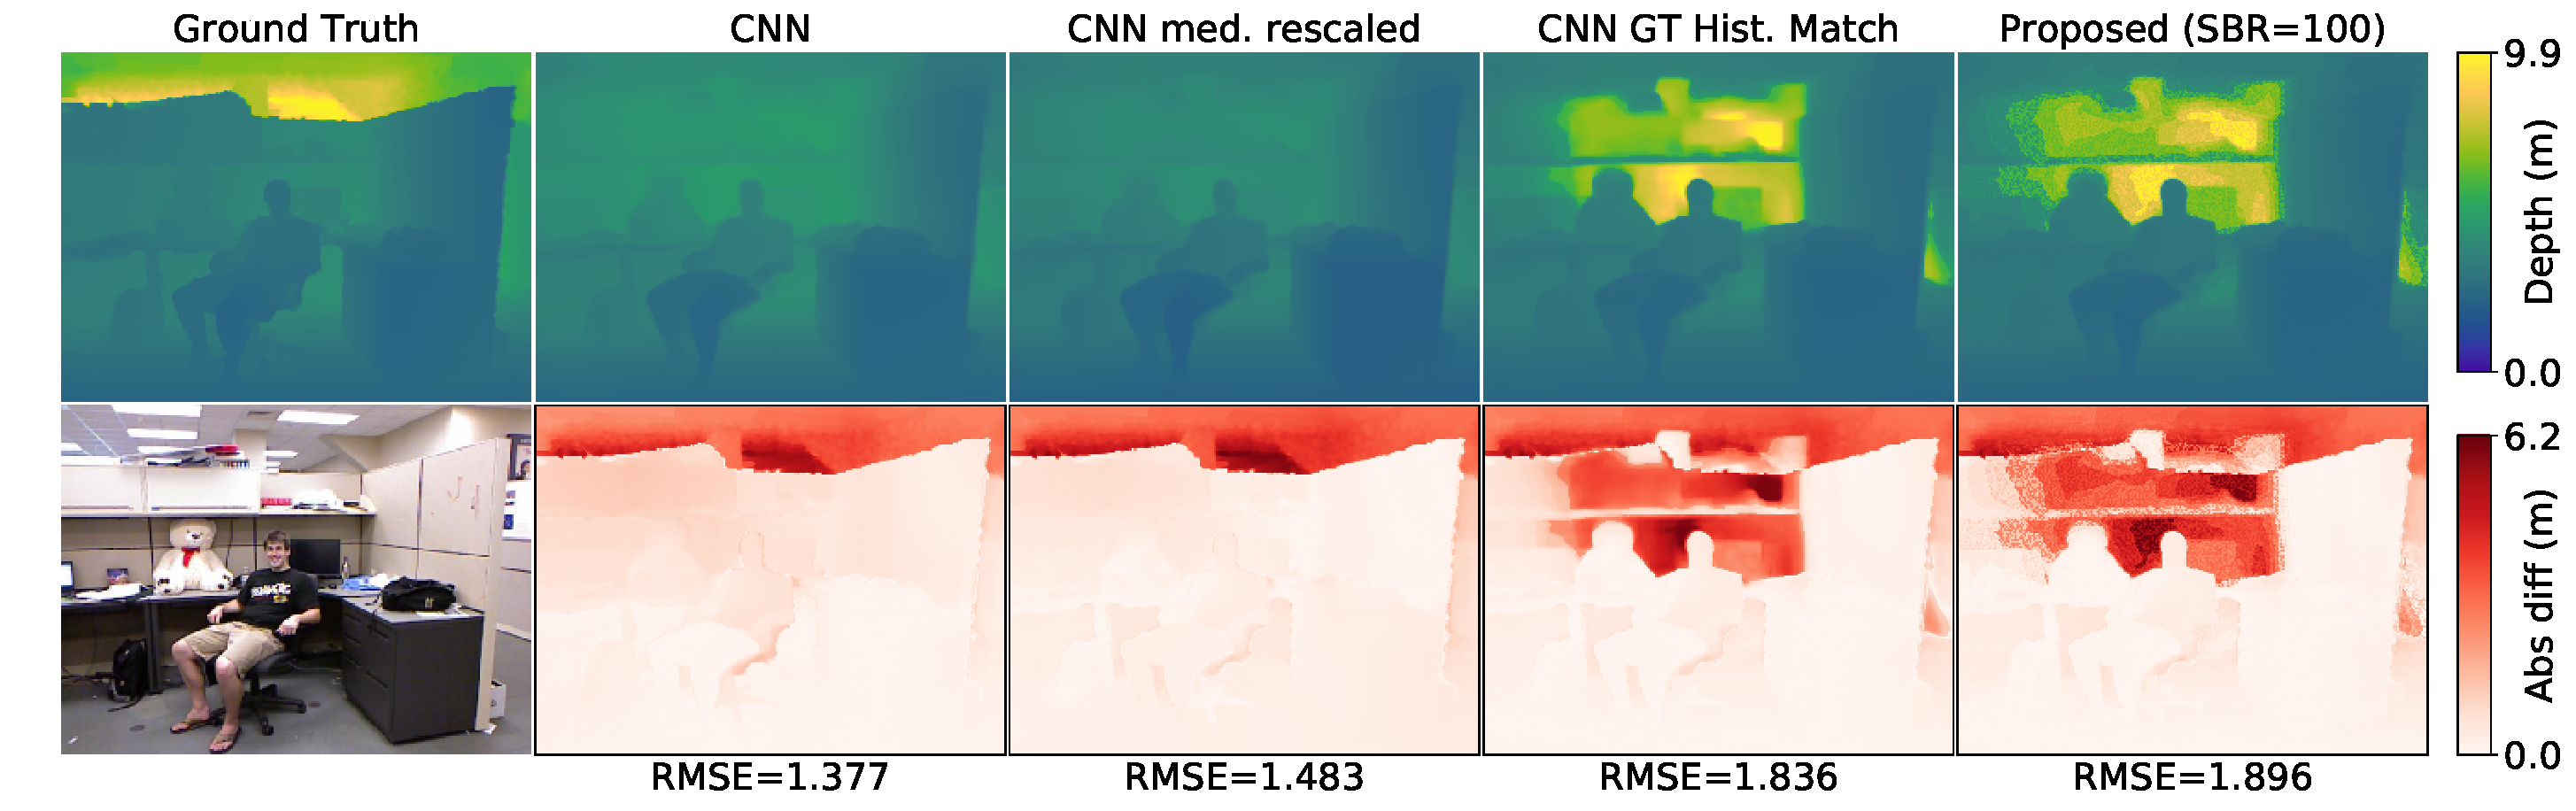
\includegraphics[height=3cm]{comparison/densedepth_258_comparison.pdf}
%   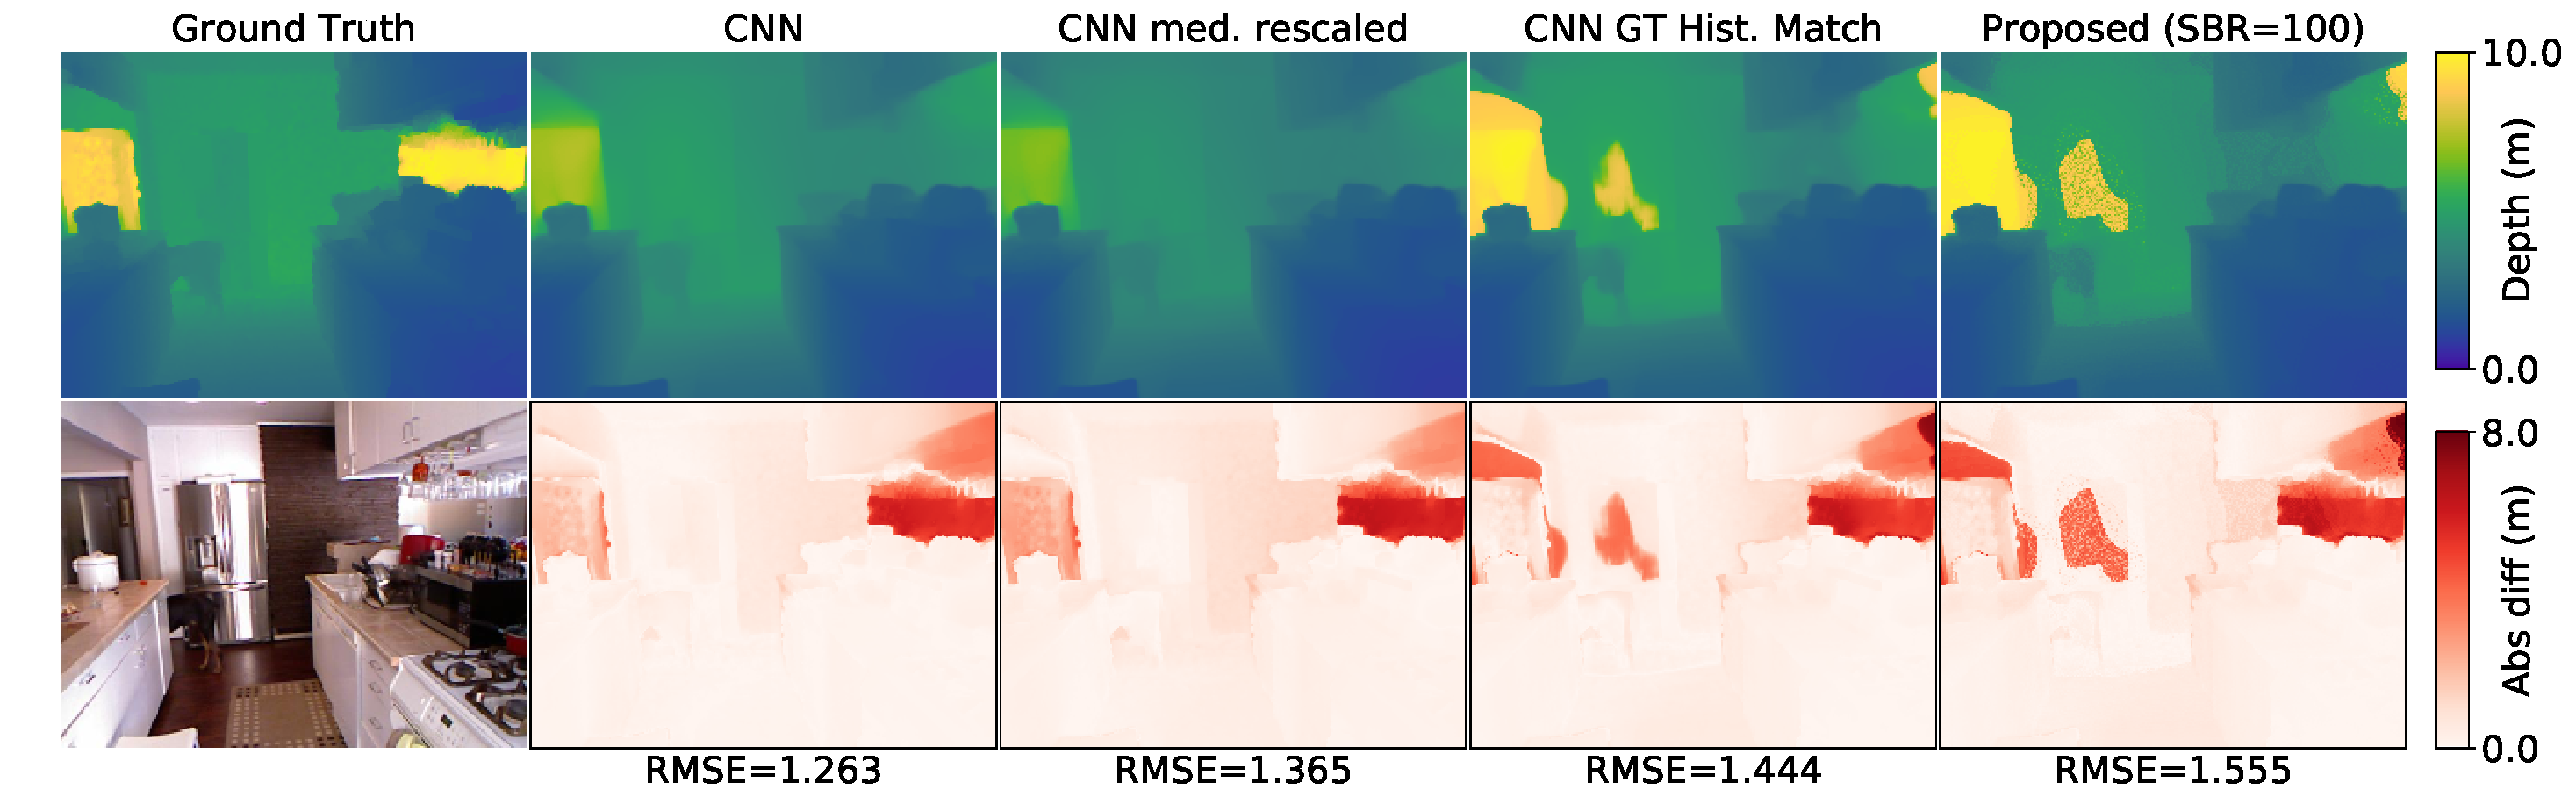
\includegraphics[height=3cm]{comparison/densedepth_341_comparison.pdf}
\begin{figure}[H]
  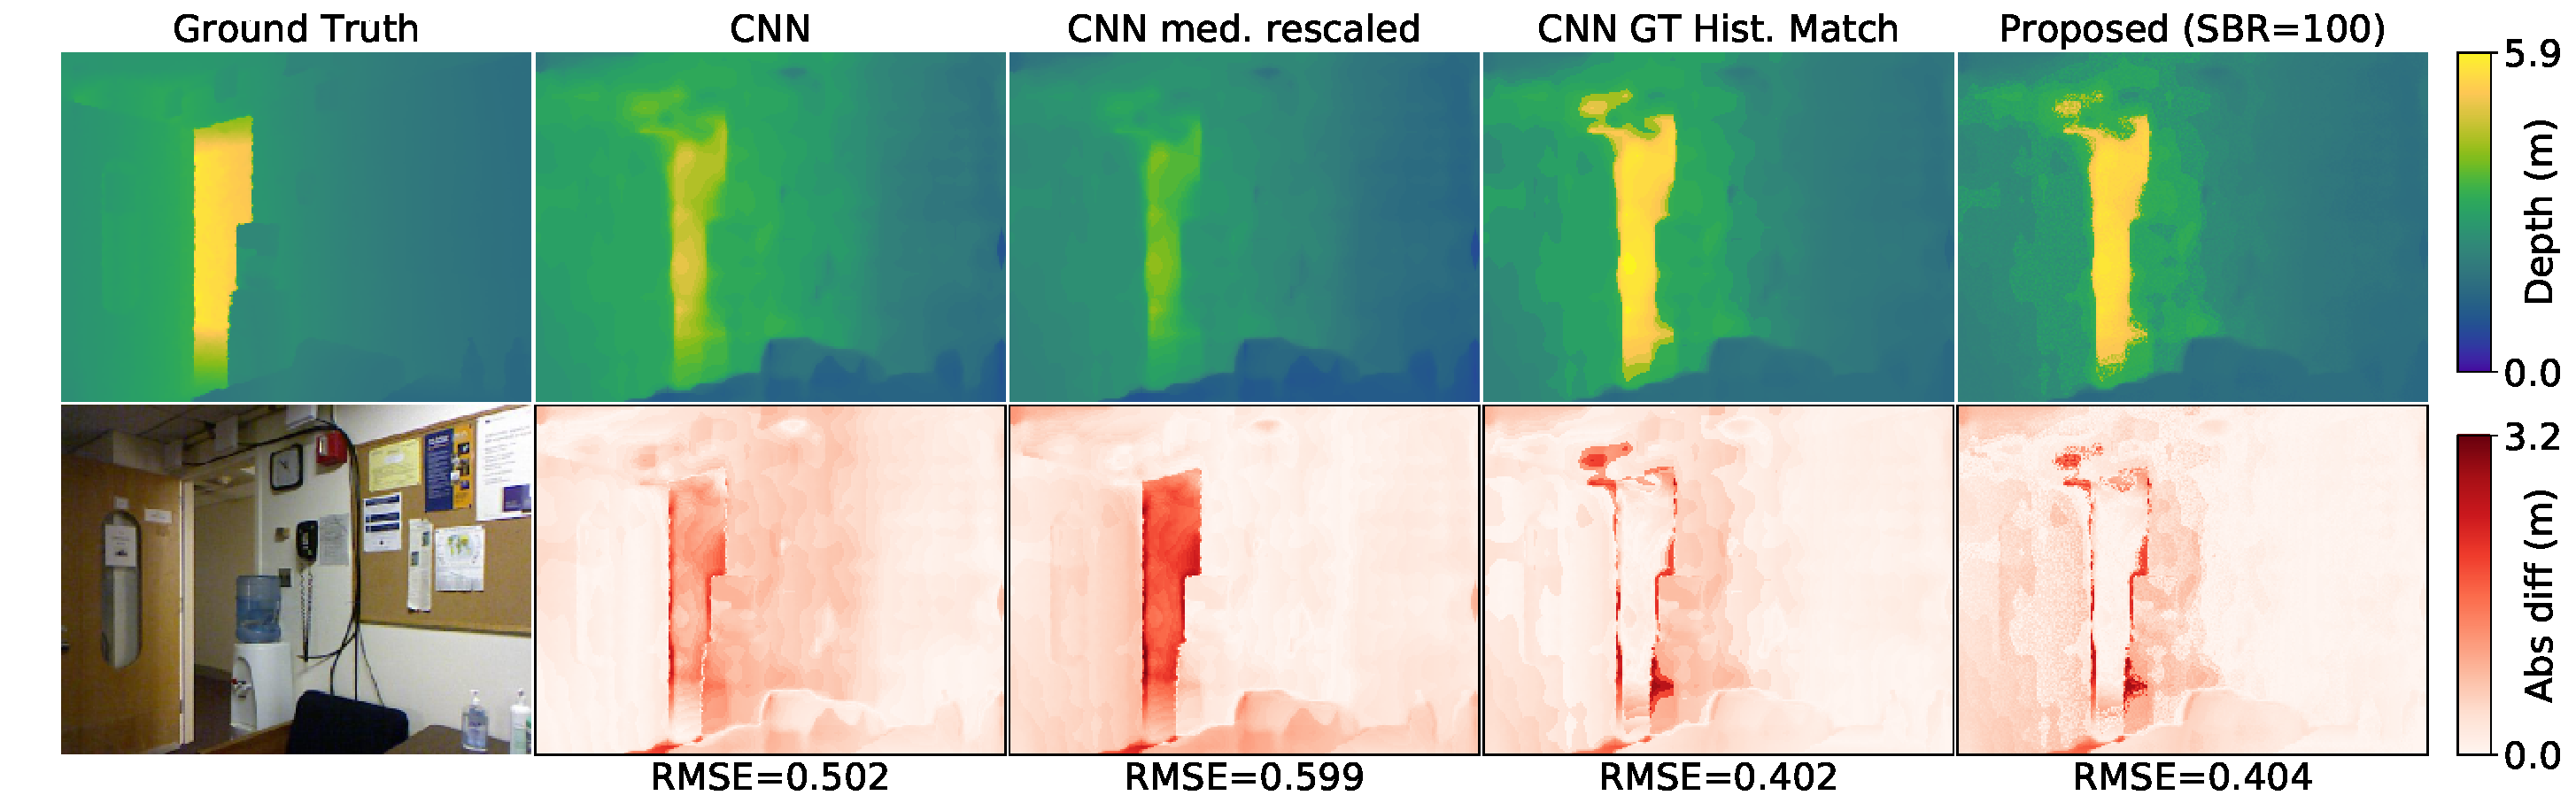
\includegraphics[width=\textwidth]{comparison/dorn_8_comparison.pdf}
  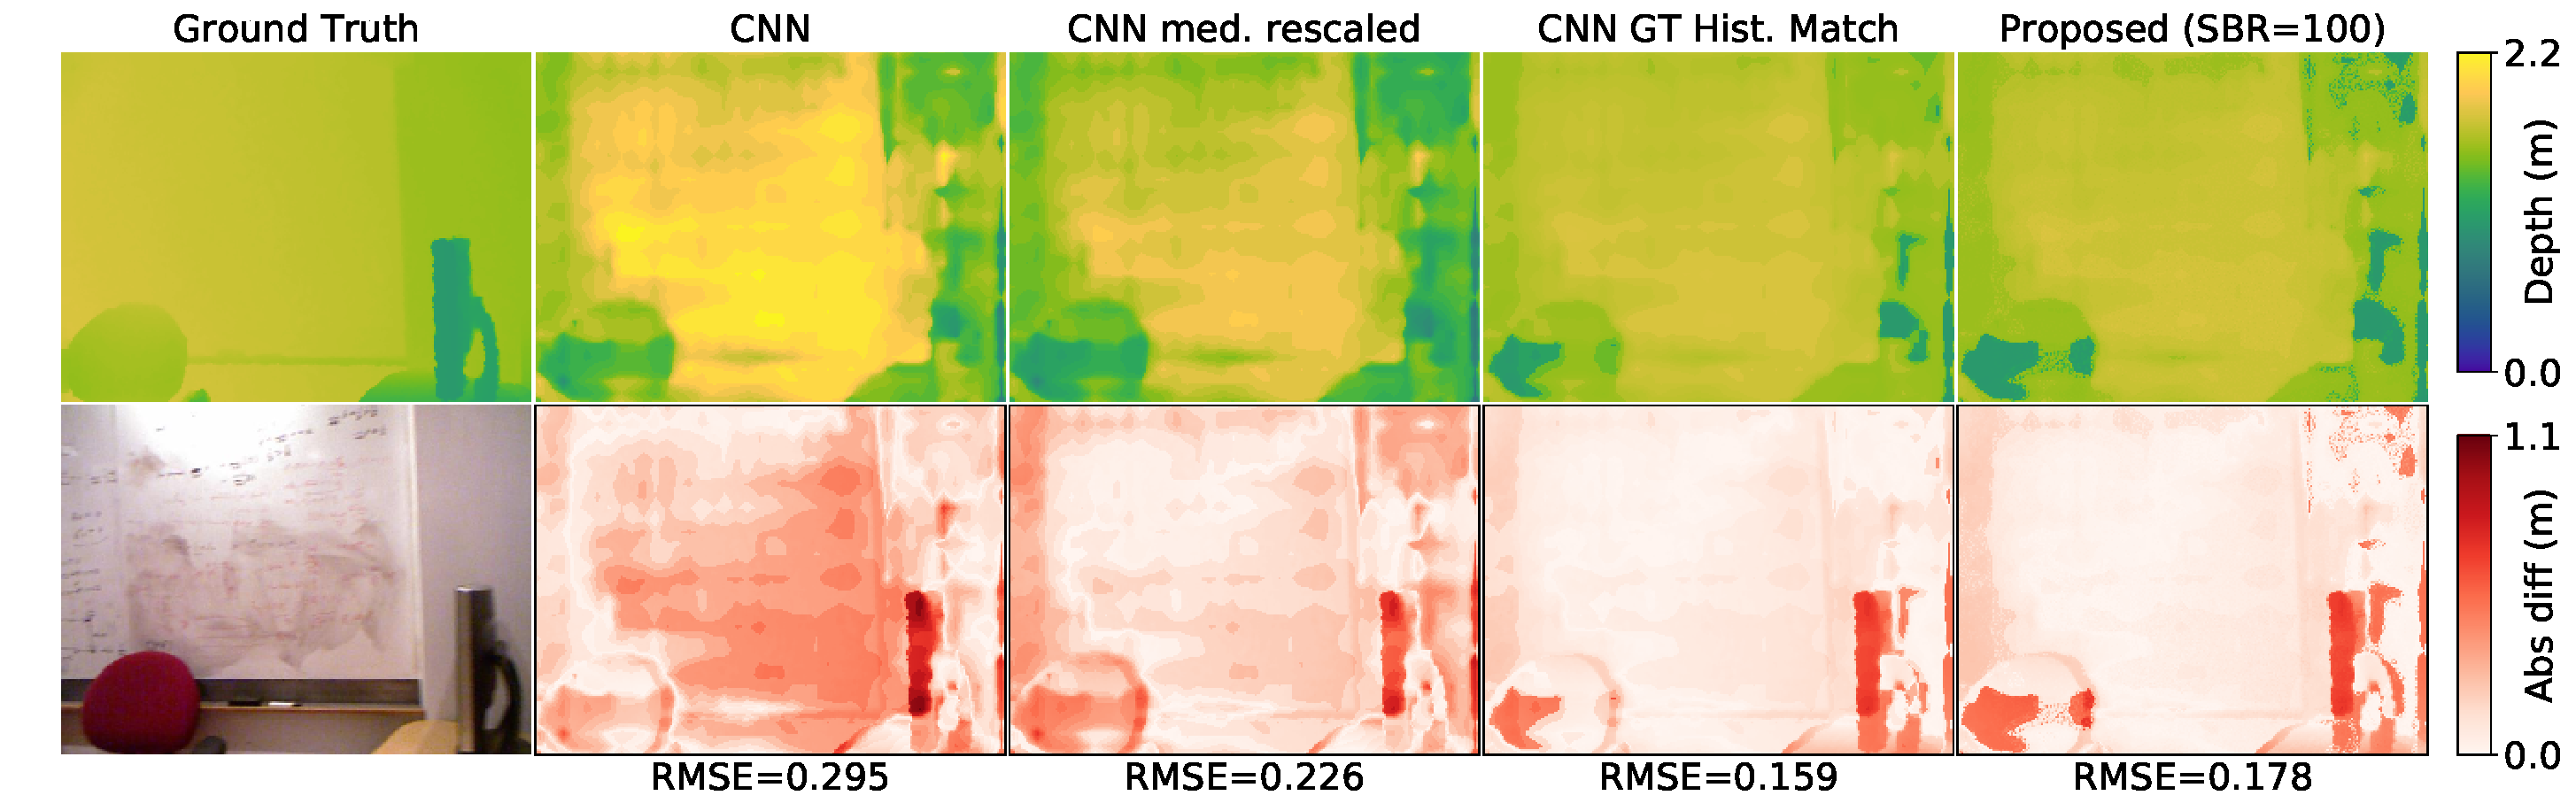
\includegraphics[width=\textwidth]{comparison/dorn_14_comparison.pdf}
  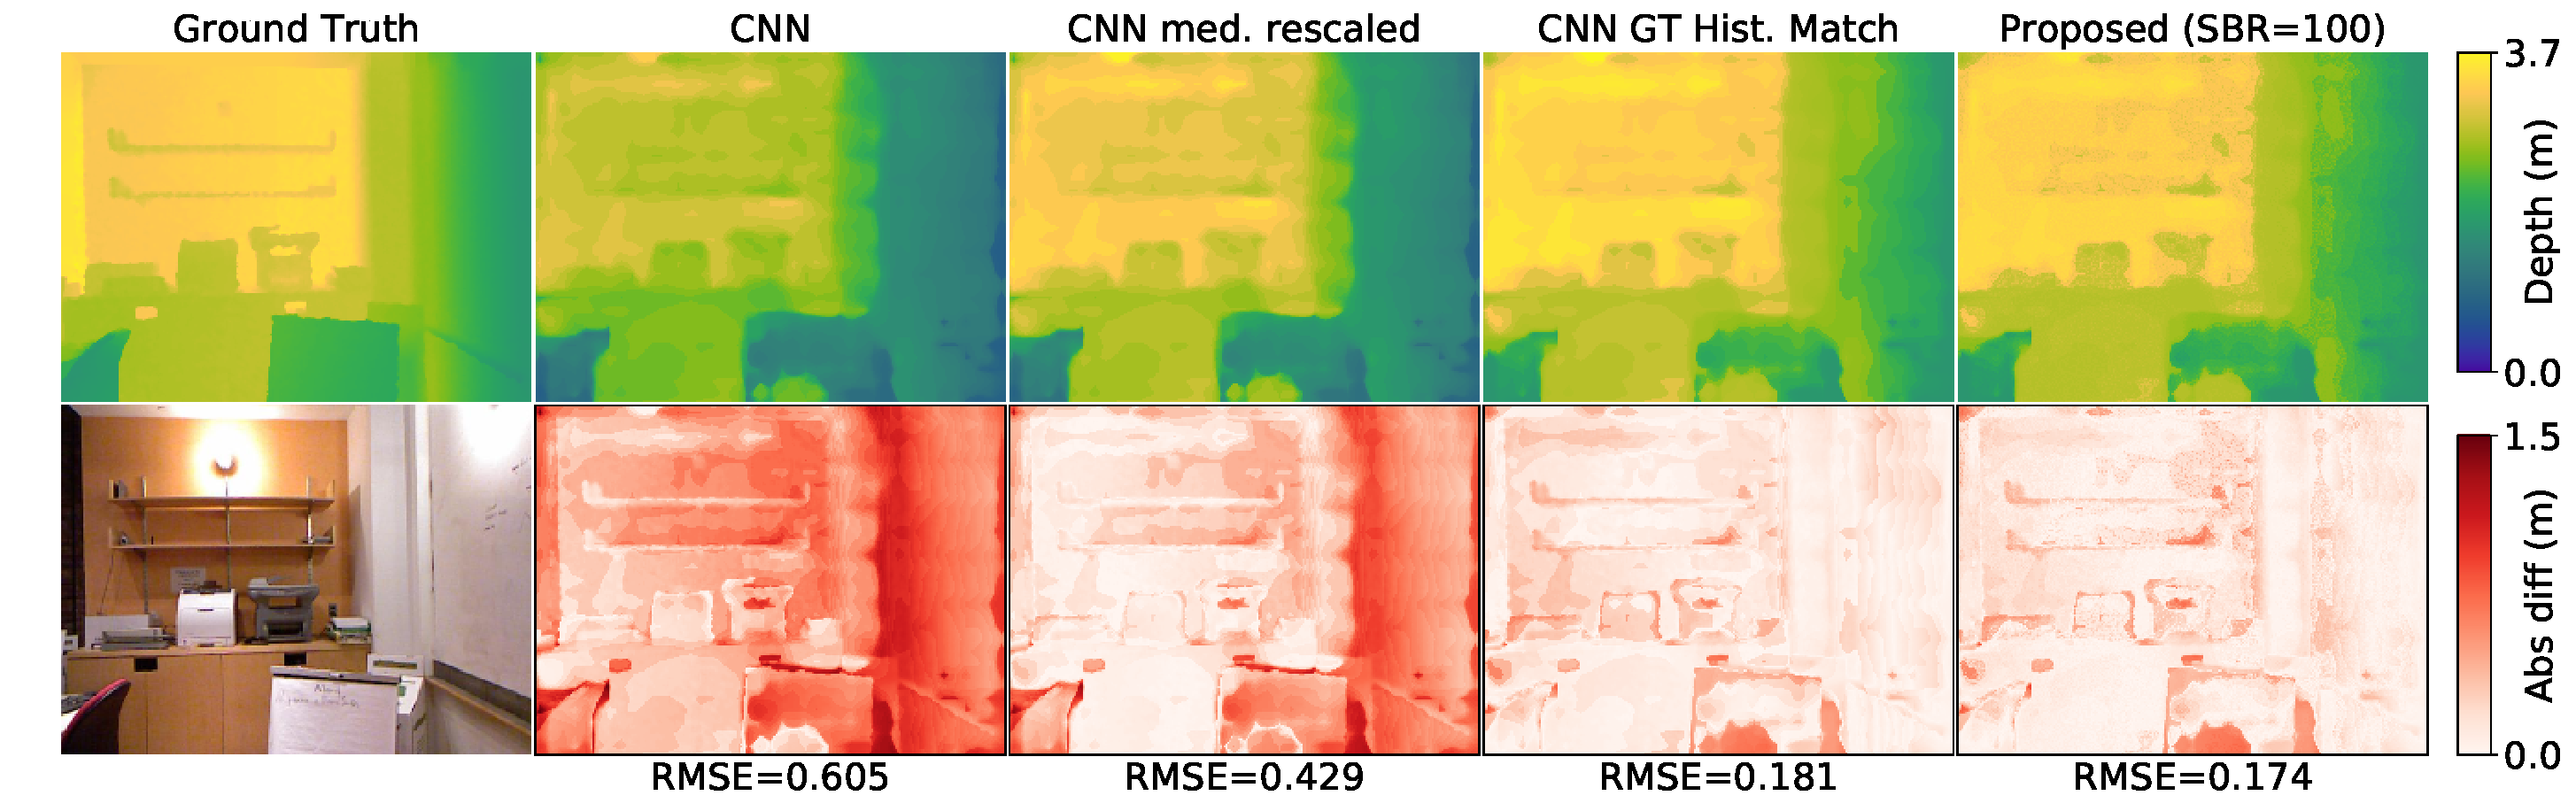
\includegraphics[width=\textwidth]{comparison/dorn_15_comparison.pdf}
  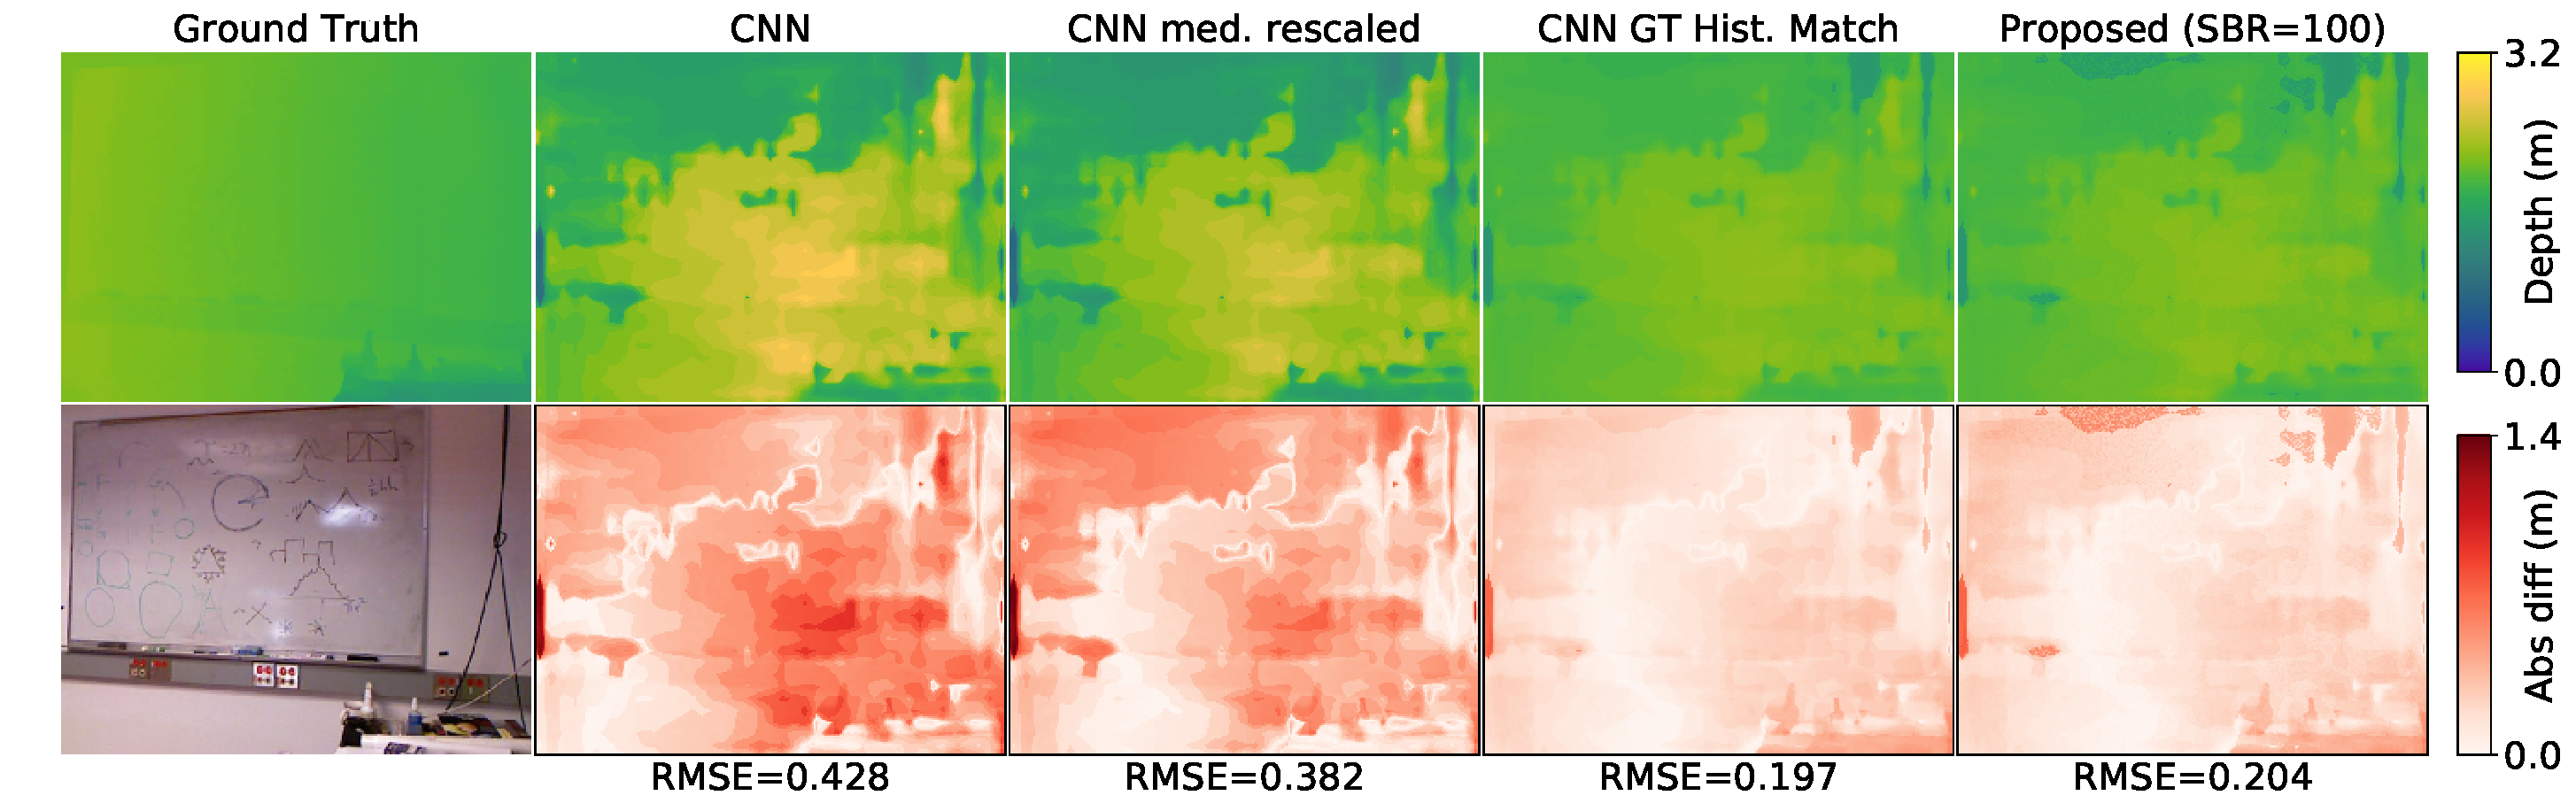
\includegraphics[width=\textwidth]{comparison/dorn_23_comparison.pdf}
  \caption{Results with DORN as the MDE. Our method is able to scale and shift
    the depth maps to mitigate gross errors in depth scaling.}
  \label{fig:dorn_1}
\end{figure}
\begin{figure}[H]
  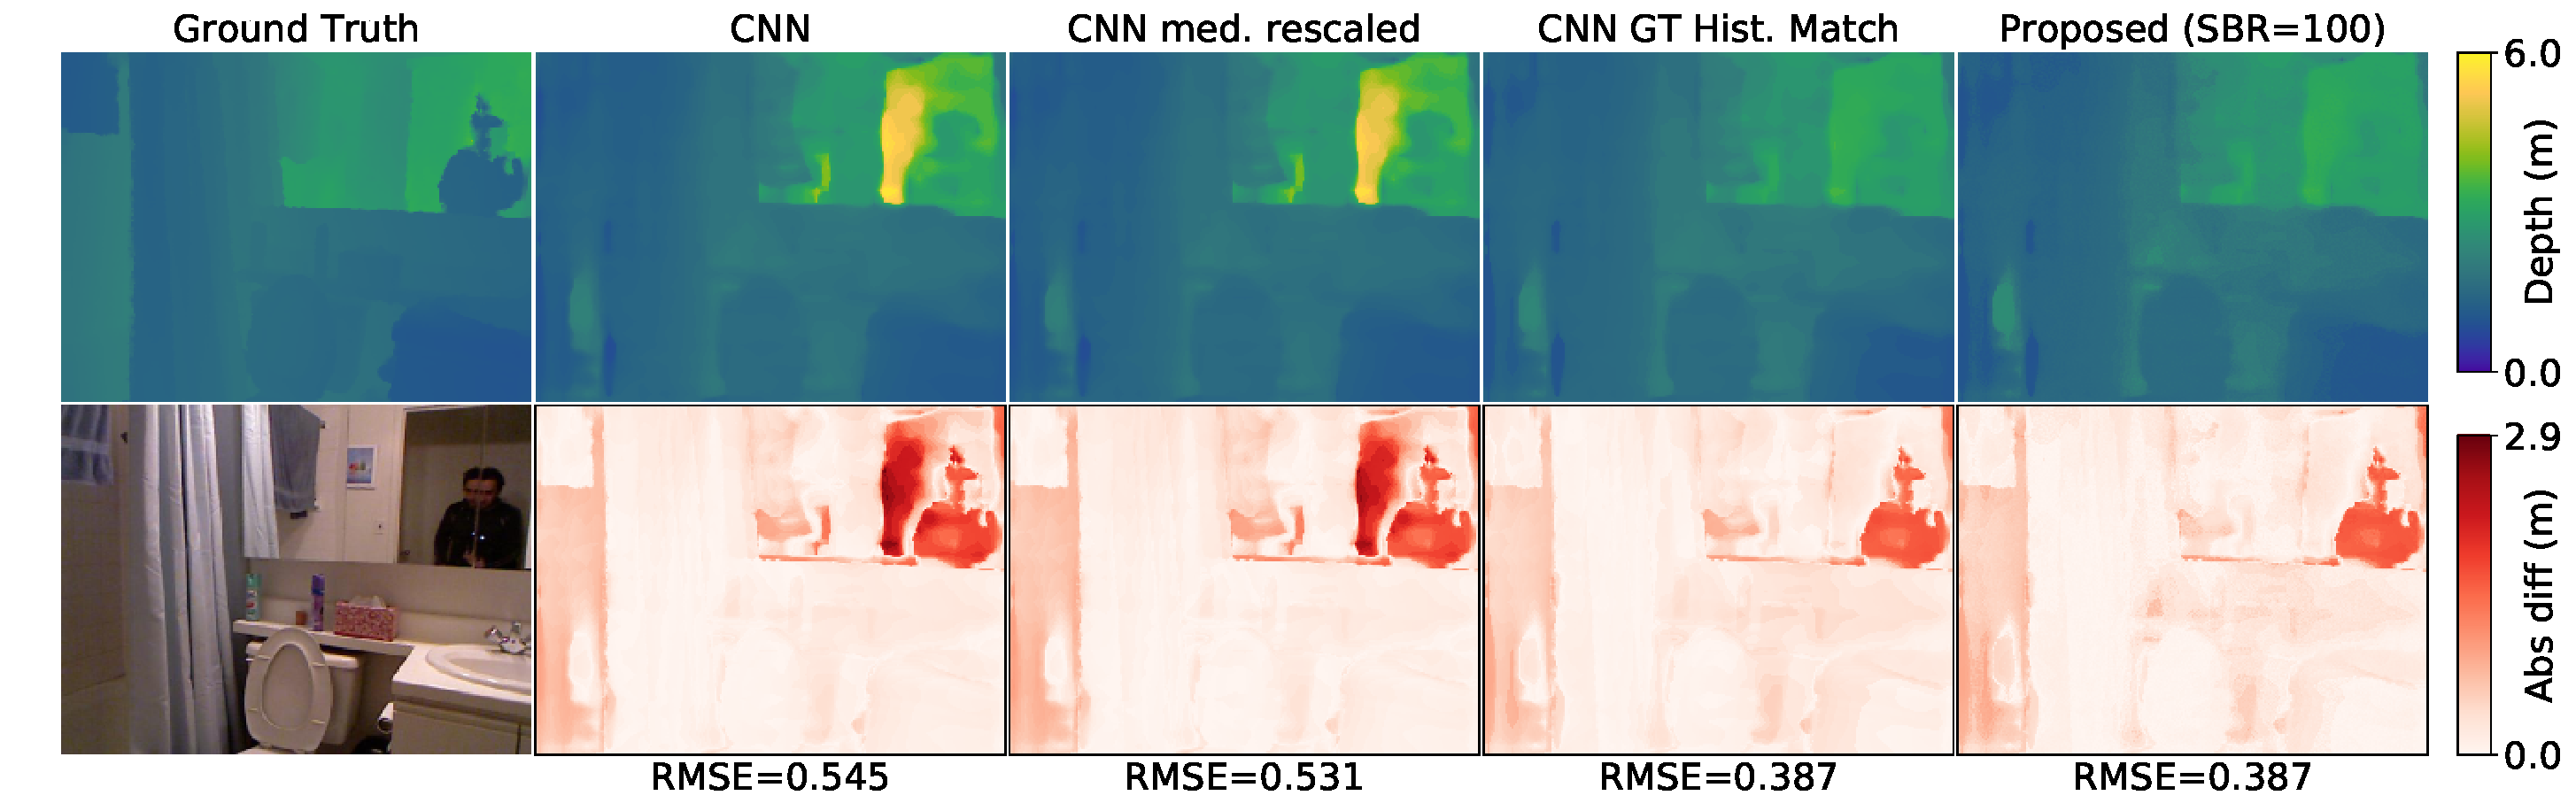
\includegraphics[width=\textwidth]{comparison/dorn_26_comparison.pdf}
  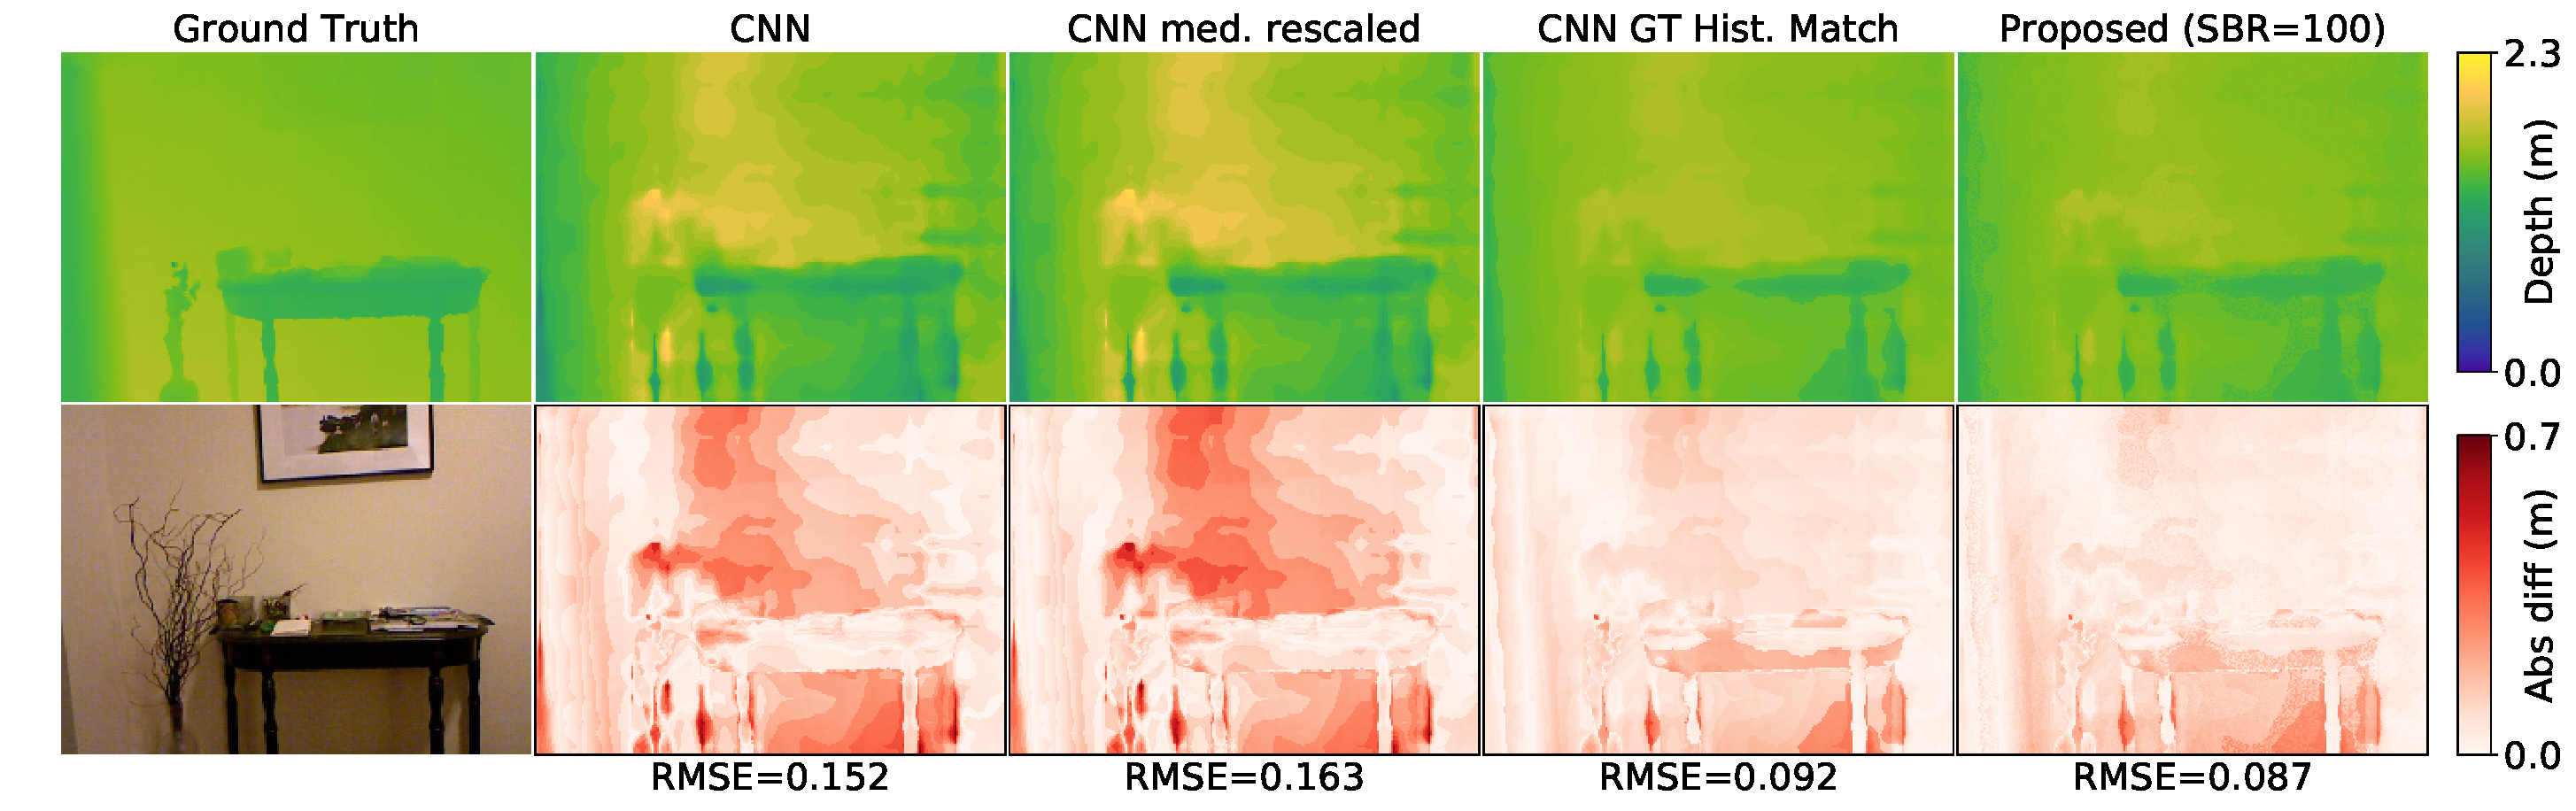
\includegraphics[width=\textwidth]{comparison/dorn_63_comparison.pdf}
  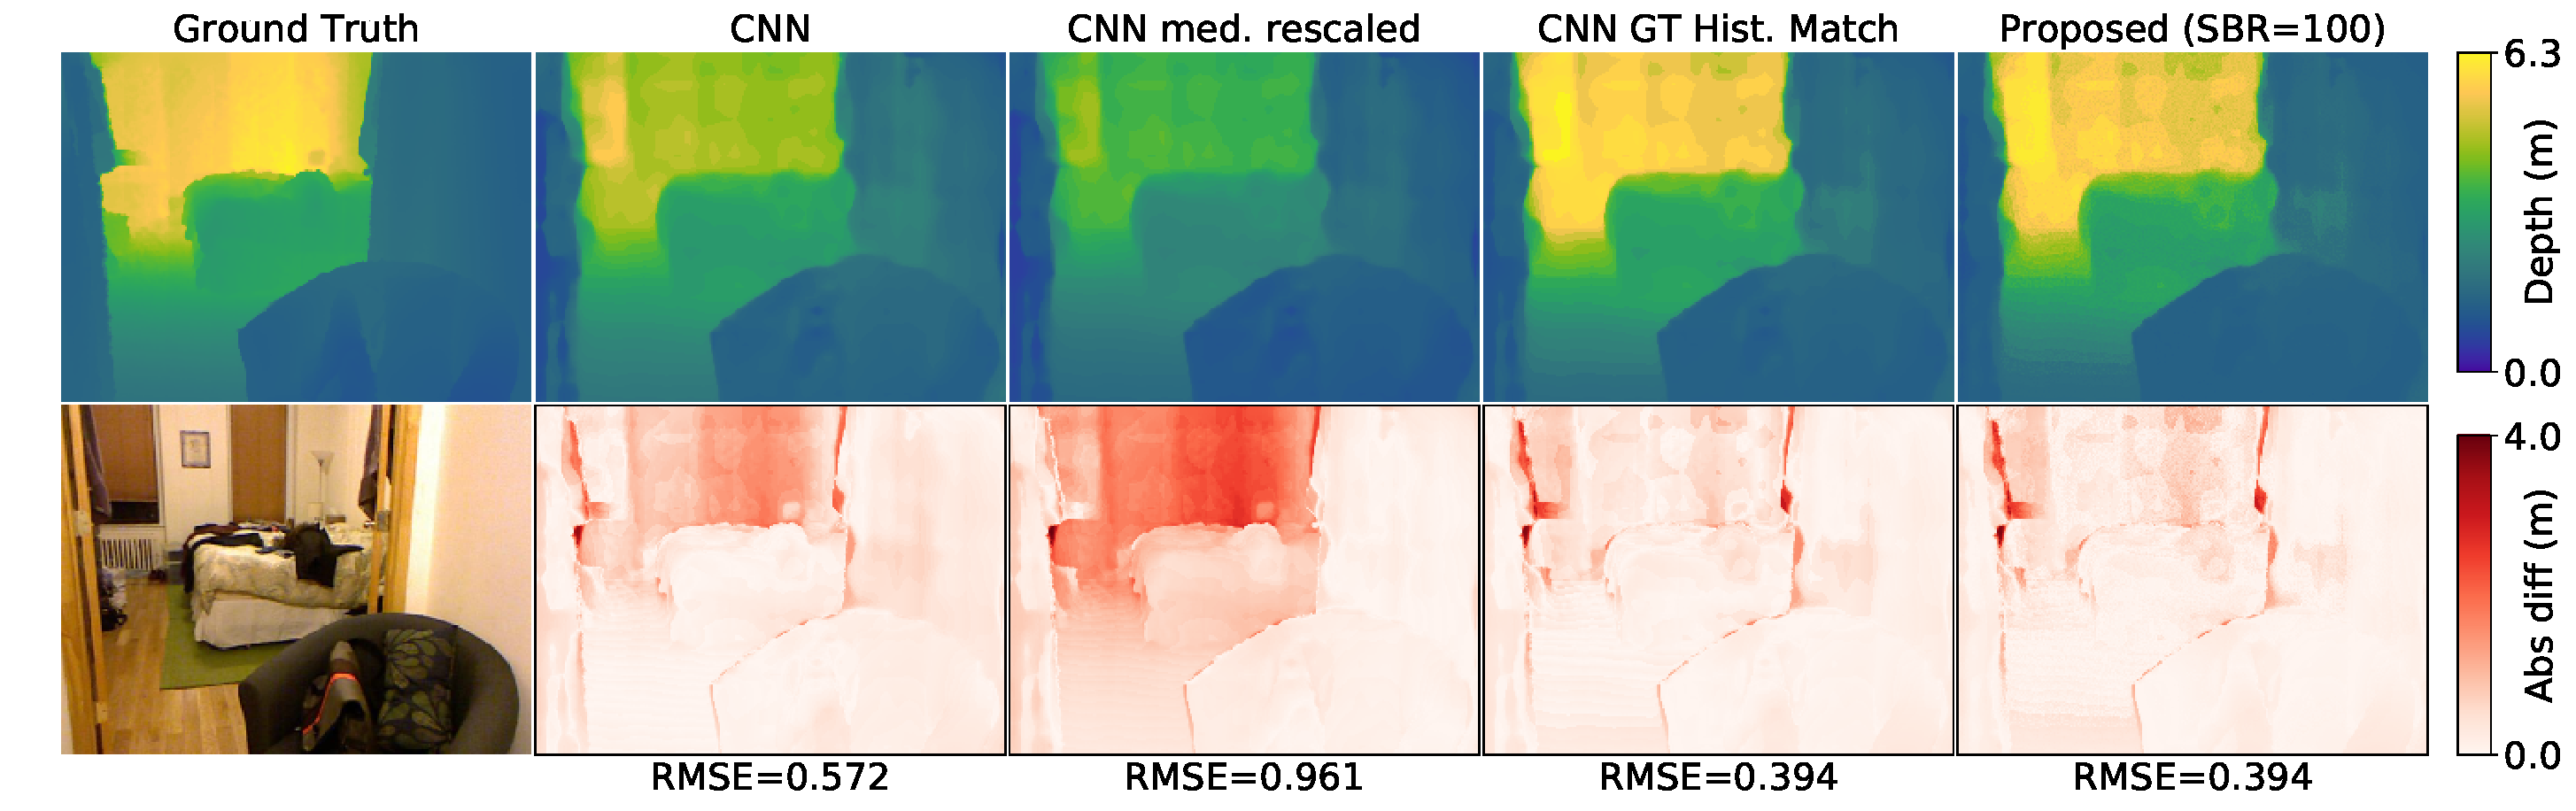
\includegraphics[width=\textwidth]{comparison/dorn_67_comparison.pdf}
  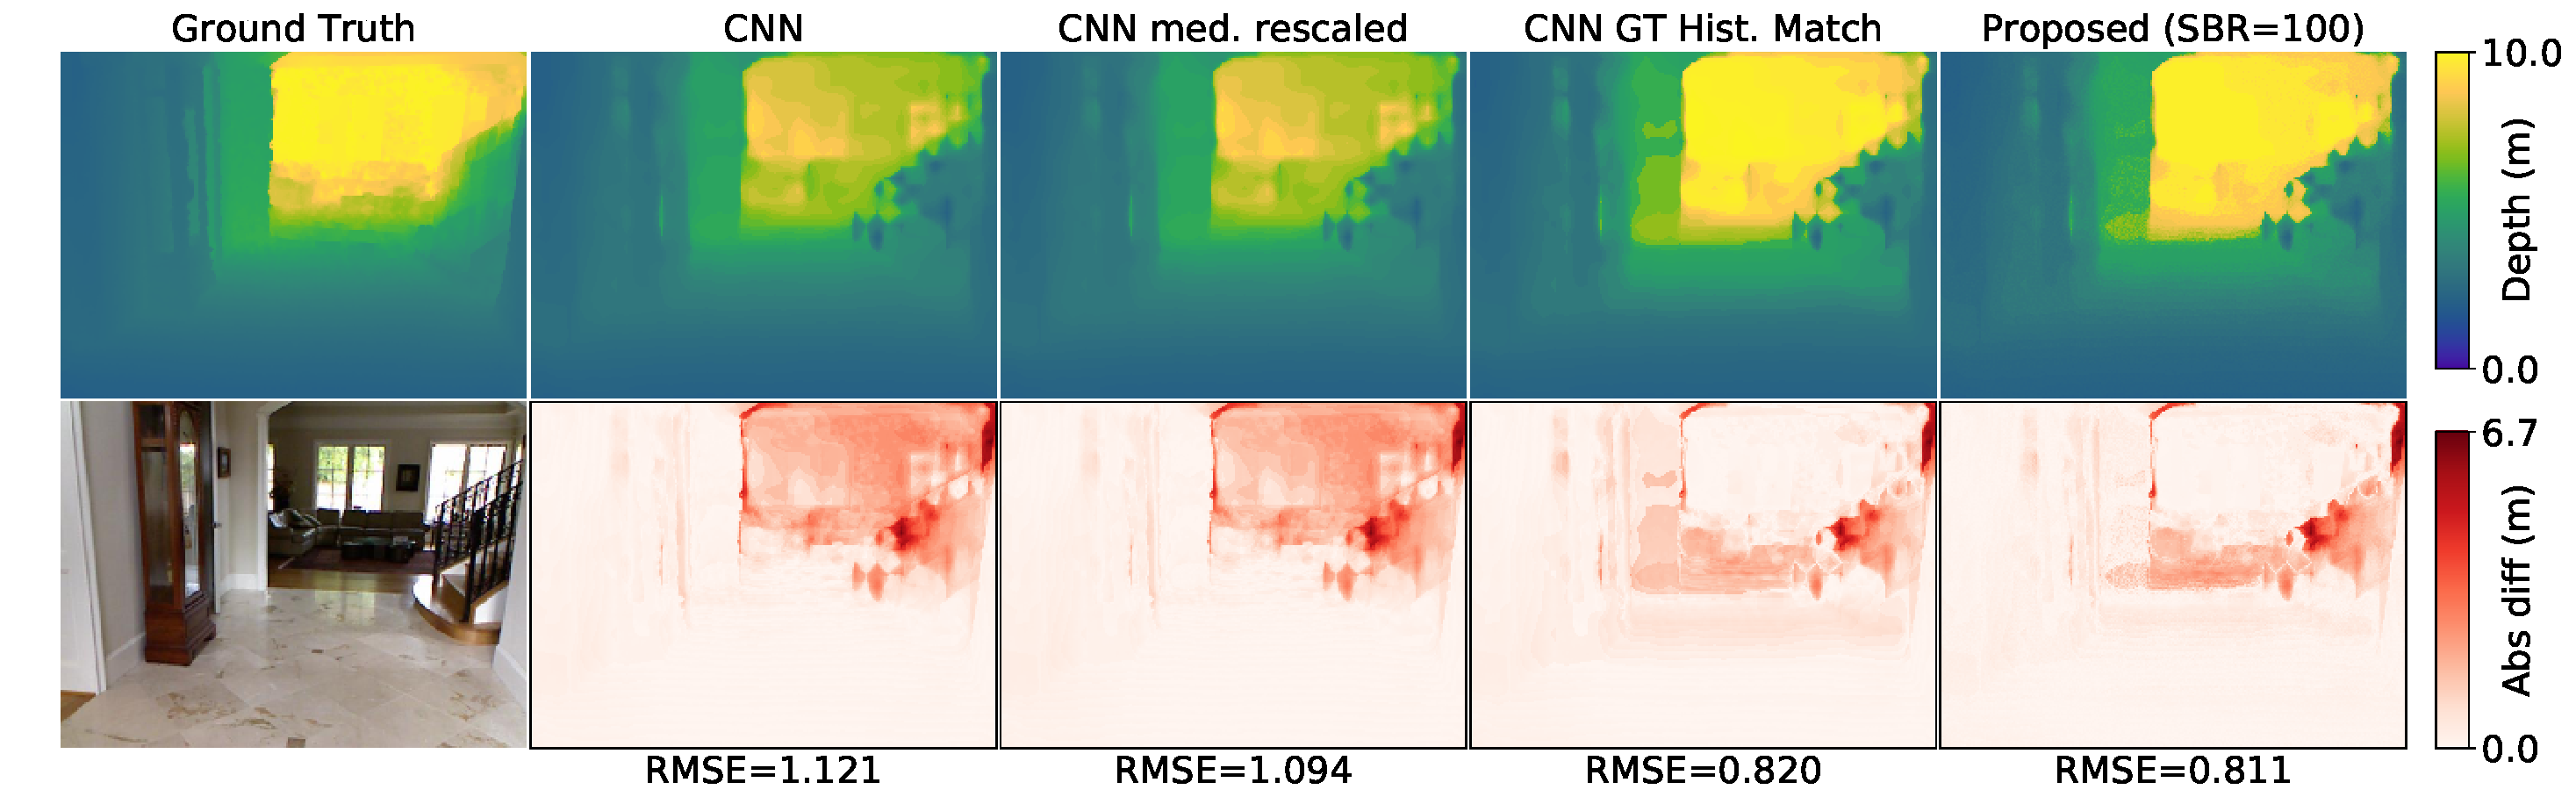
\includegraphics[width=\textwidth]{comparison/dorn_140_comparison.pdf}
  \caption{Results with DORN as the MDE. Our method is able to scale and shift
    the depth maps to mitigate gross errors in depth scaling.}
  \label{fig:dorn_2}
\end{figure}
\begin{figure}[H]
  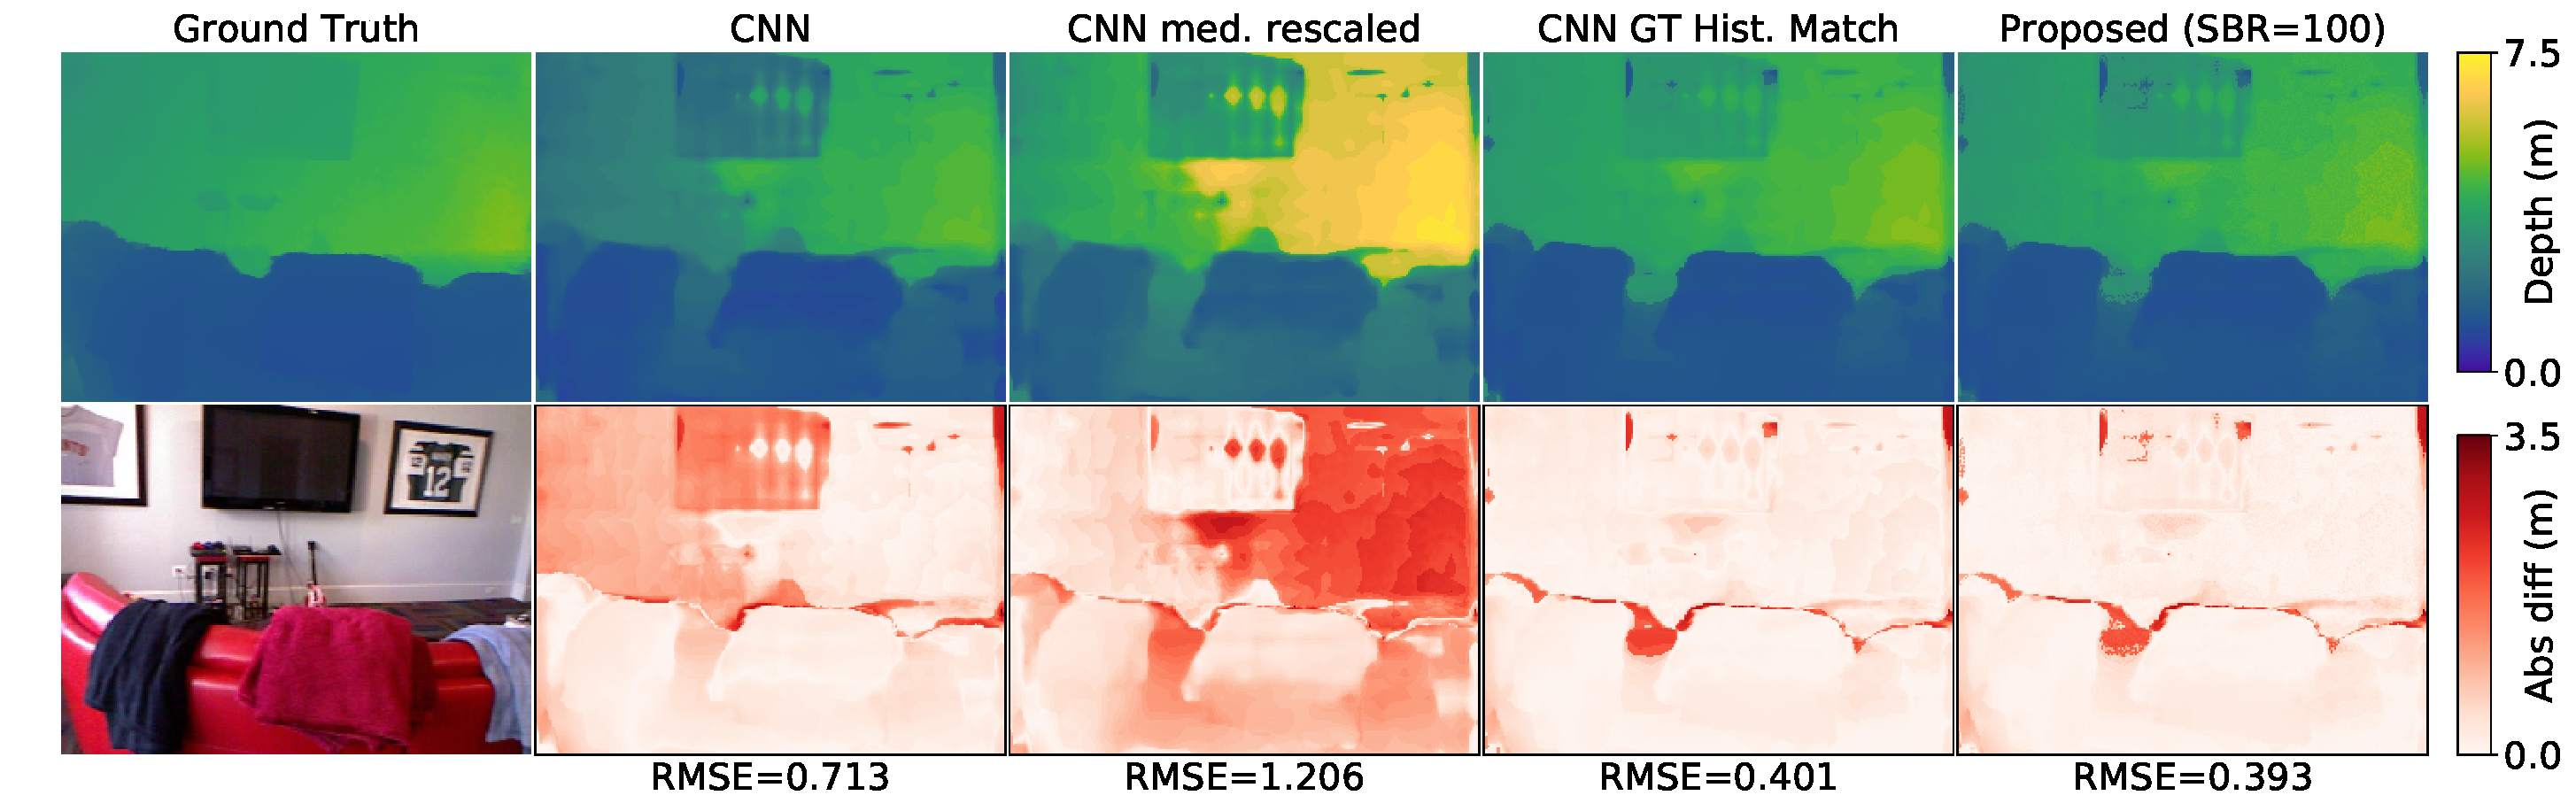
\includegraphics[width=\textwidth]{comparison/dorn_170_comparison.pdf}
  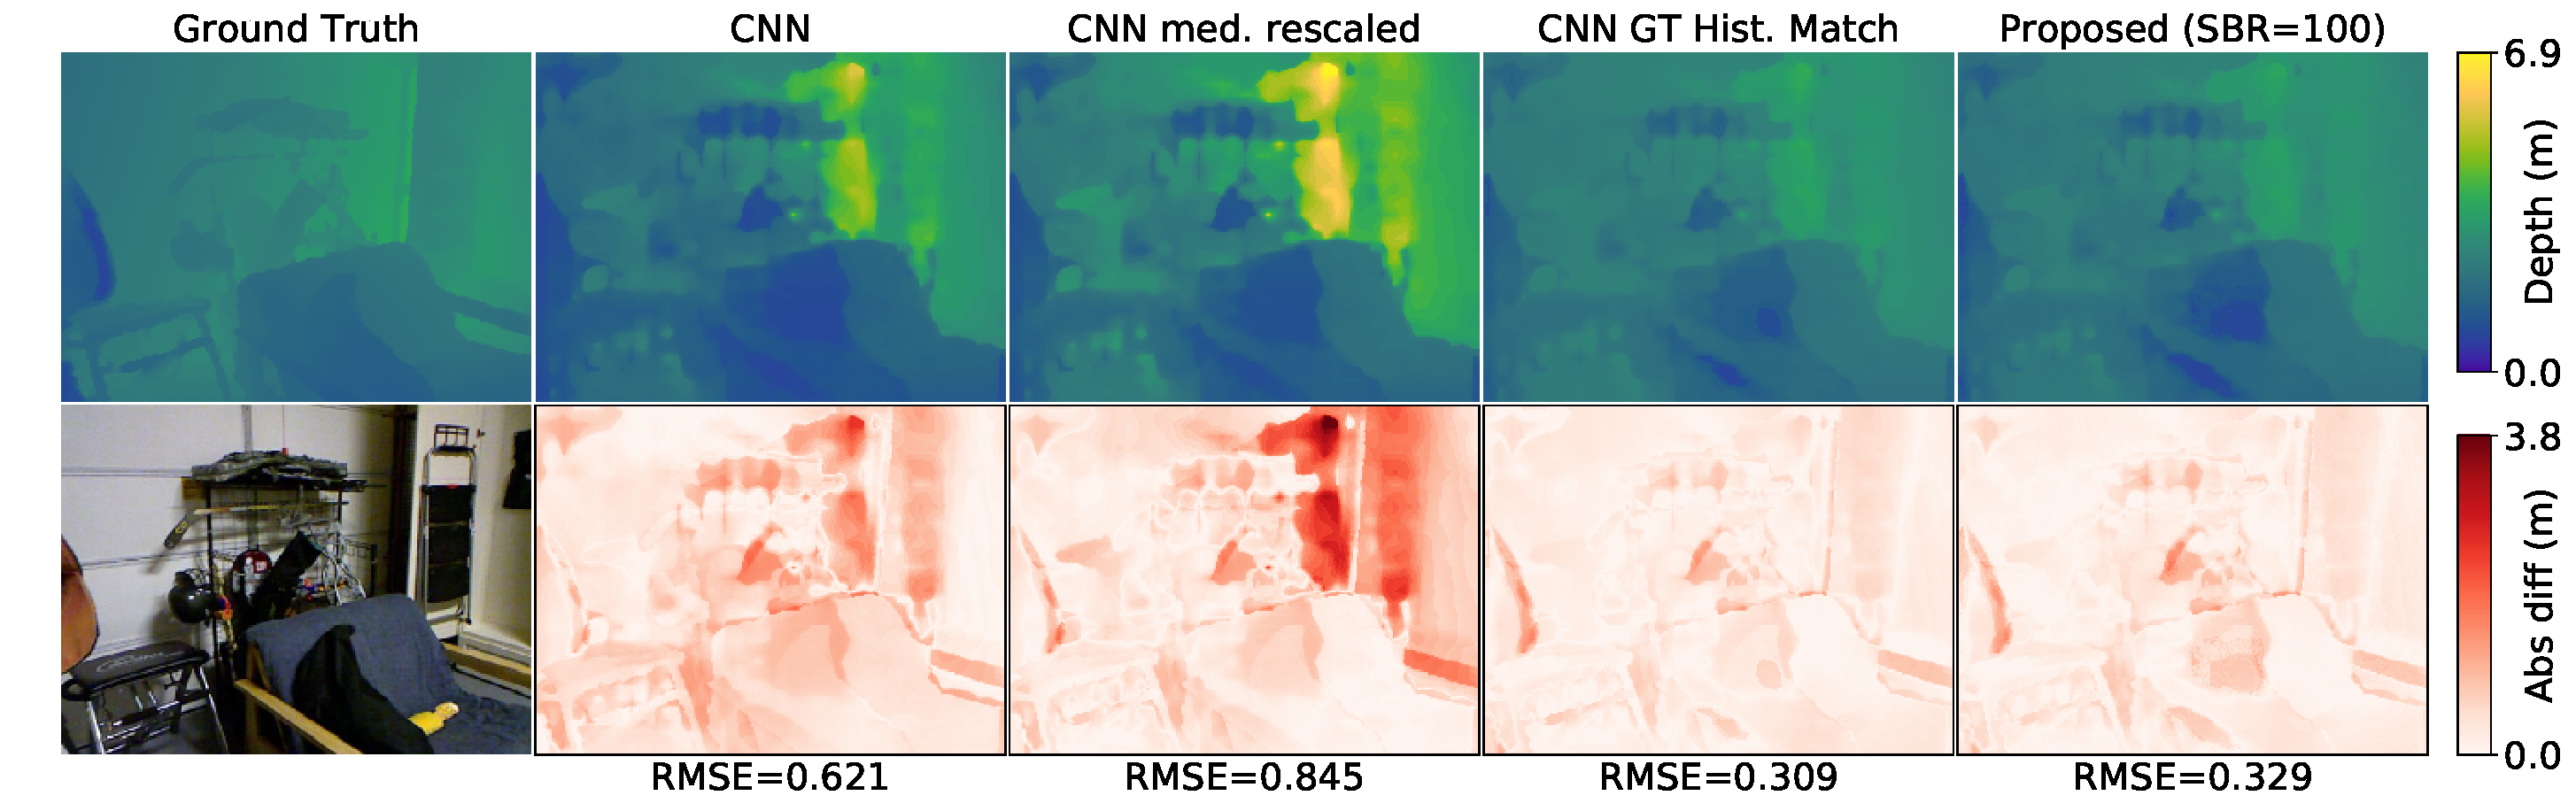
\includegraphics[width=\textwidth]{comparison/dorn_522_comparison.pdf}
  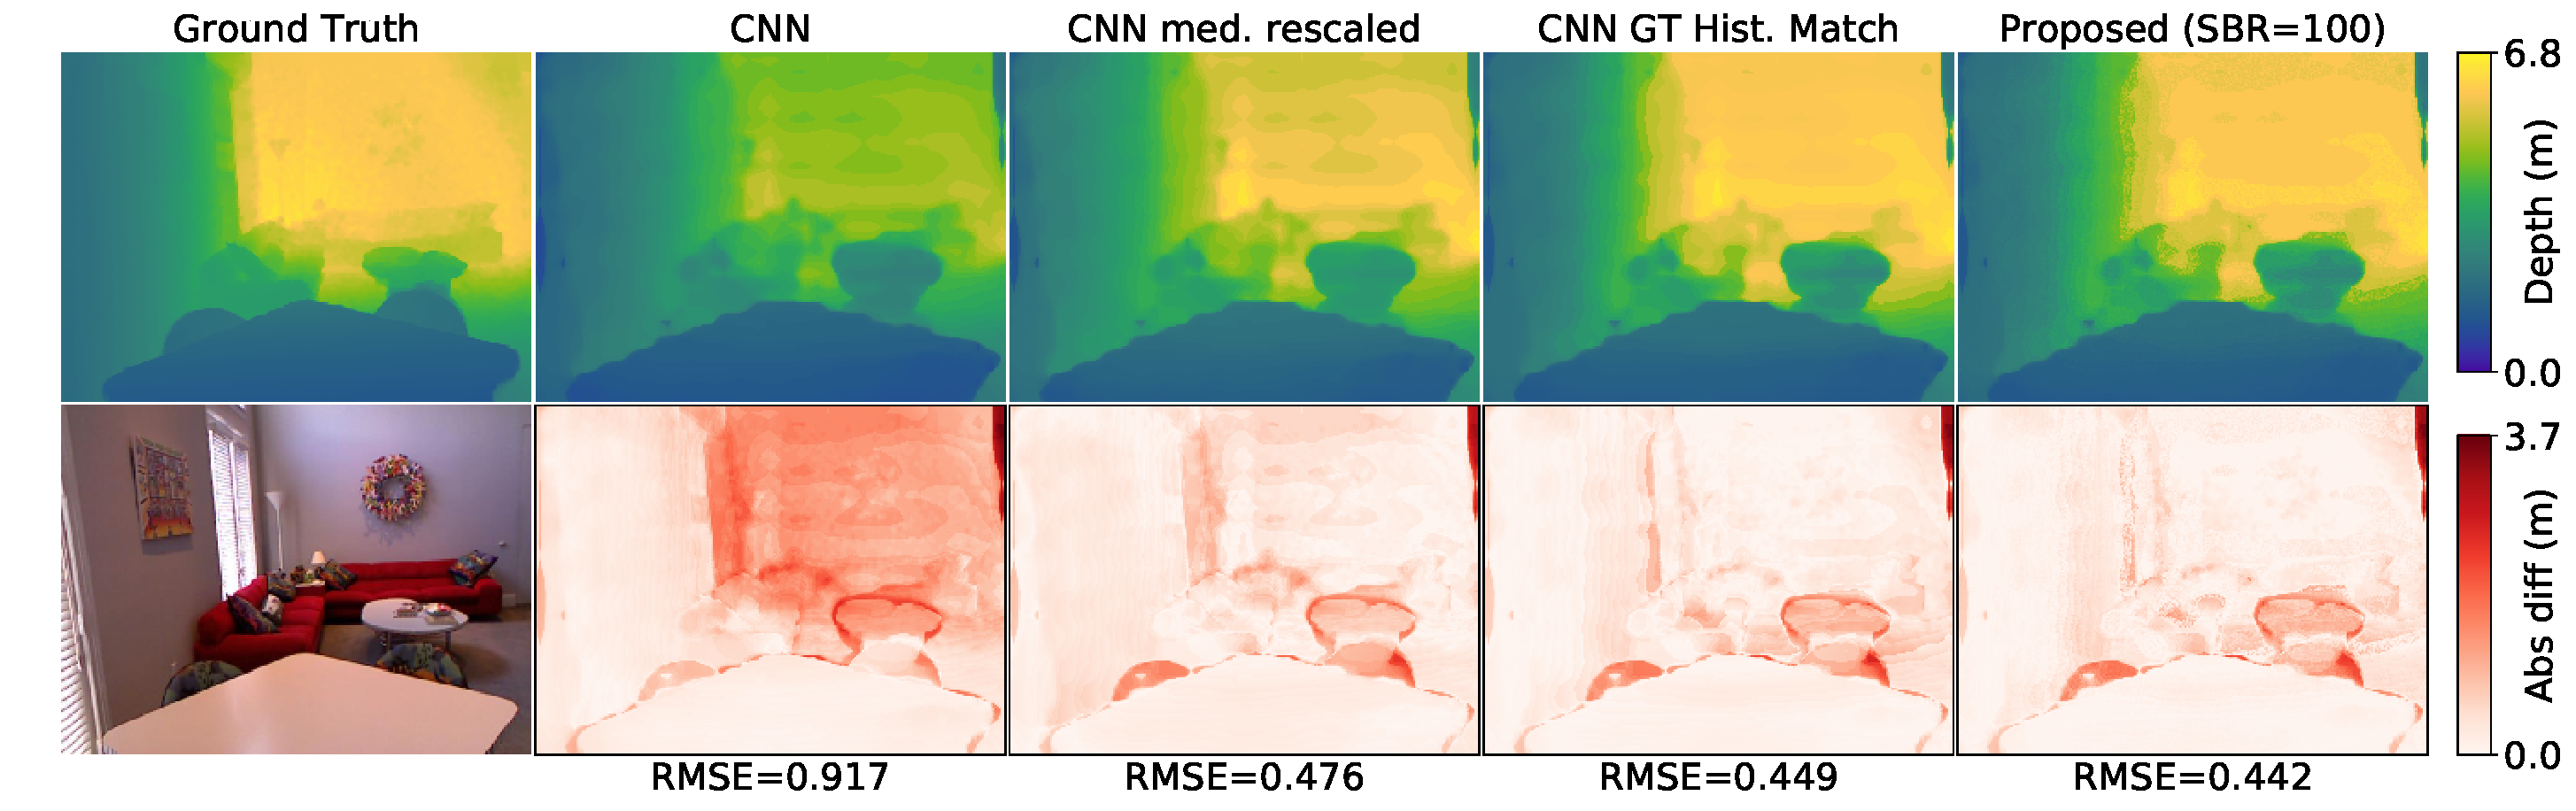
\includegraphics[width=\textwidth]{comparison/dorn_548_comparison.pdf}
  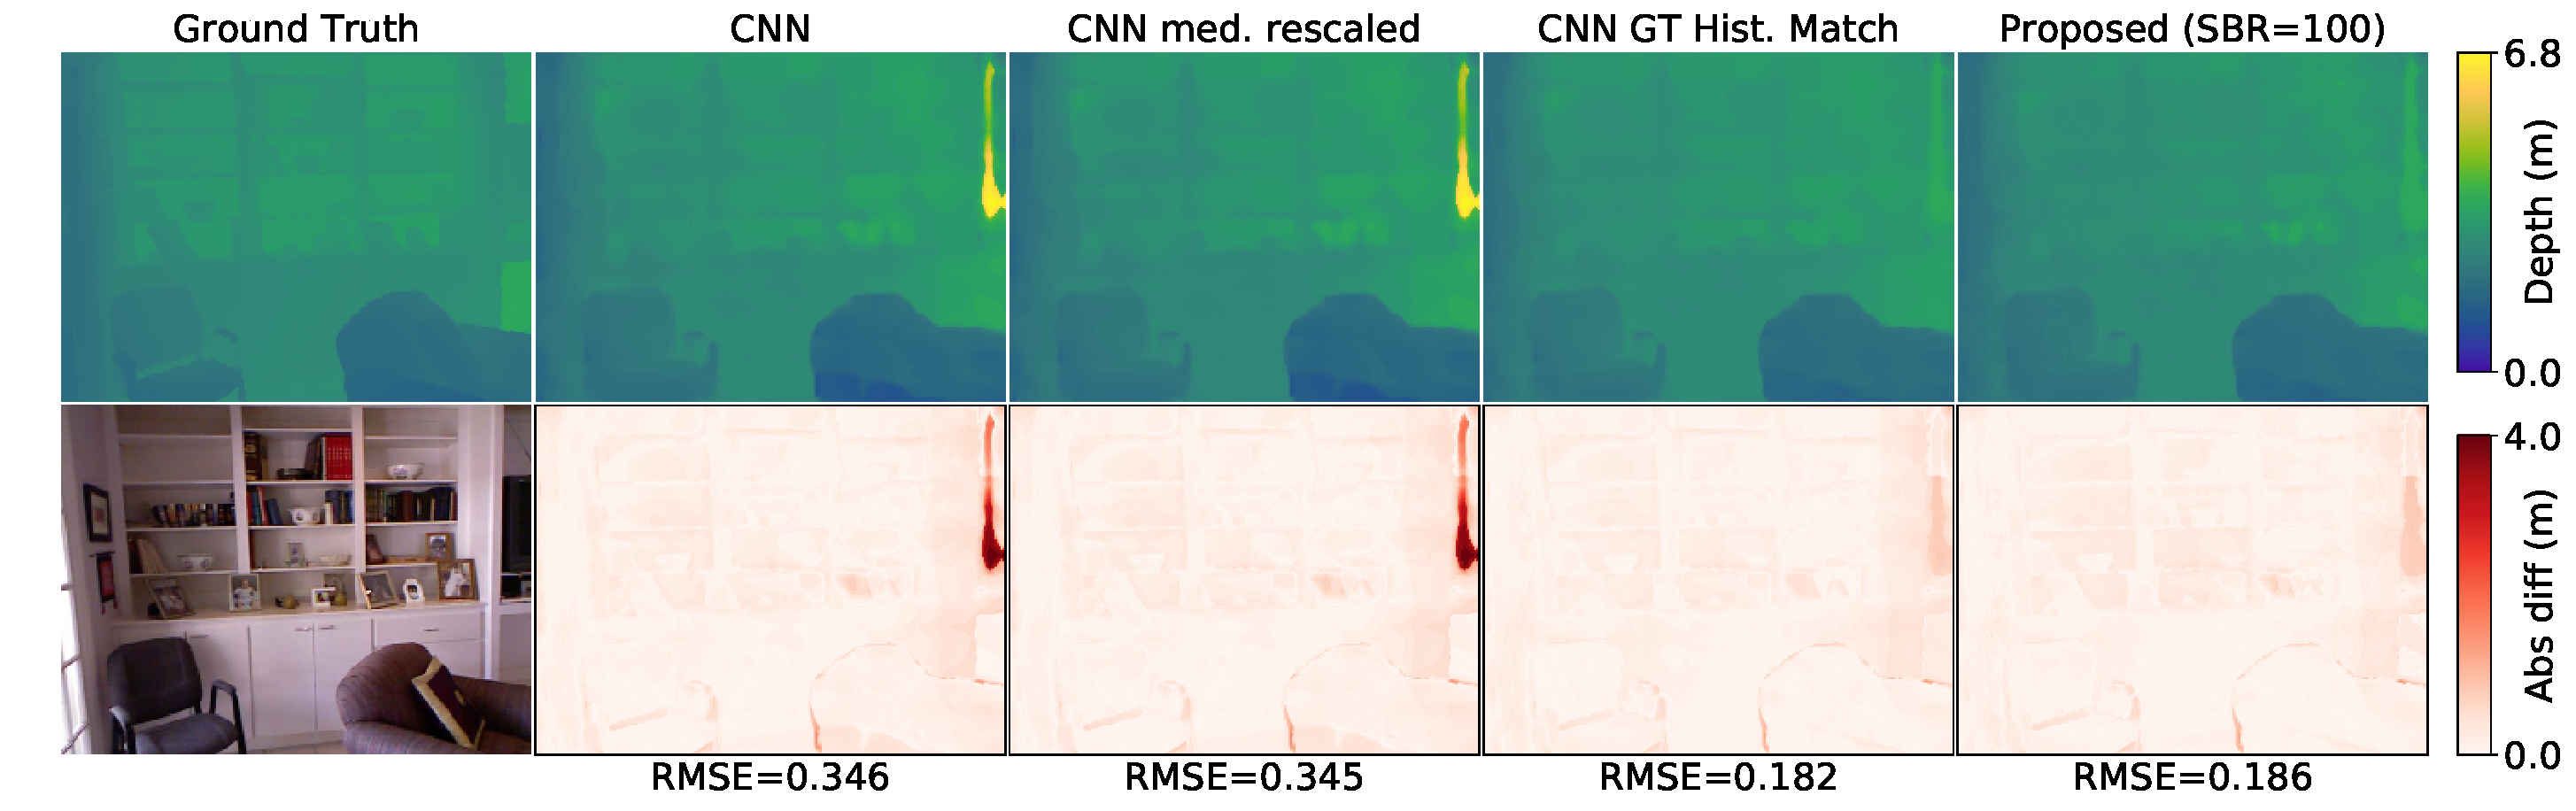
\includegraphics[width=\textwidth]{comparison/dorn_569_comparison.pdf}
  \caption{Results with DORN as the MDE. Our method is able to scale and shift
    the depth maps to mitigate gross errors in depth scaling.}
  \label{fig:dorn_3}
\end{figure}
% \begin{figure}
%   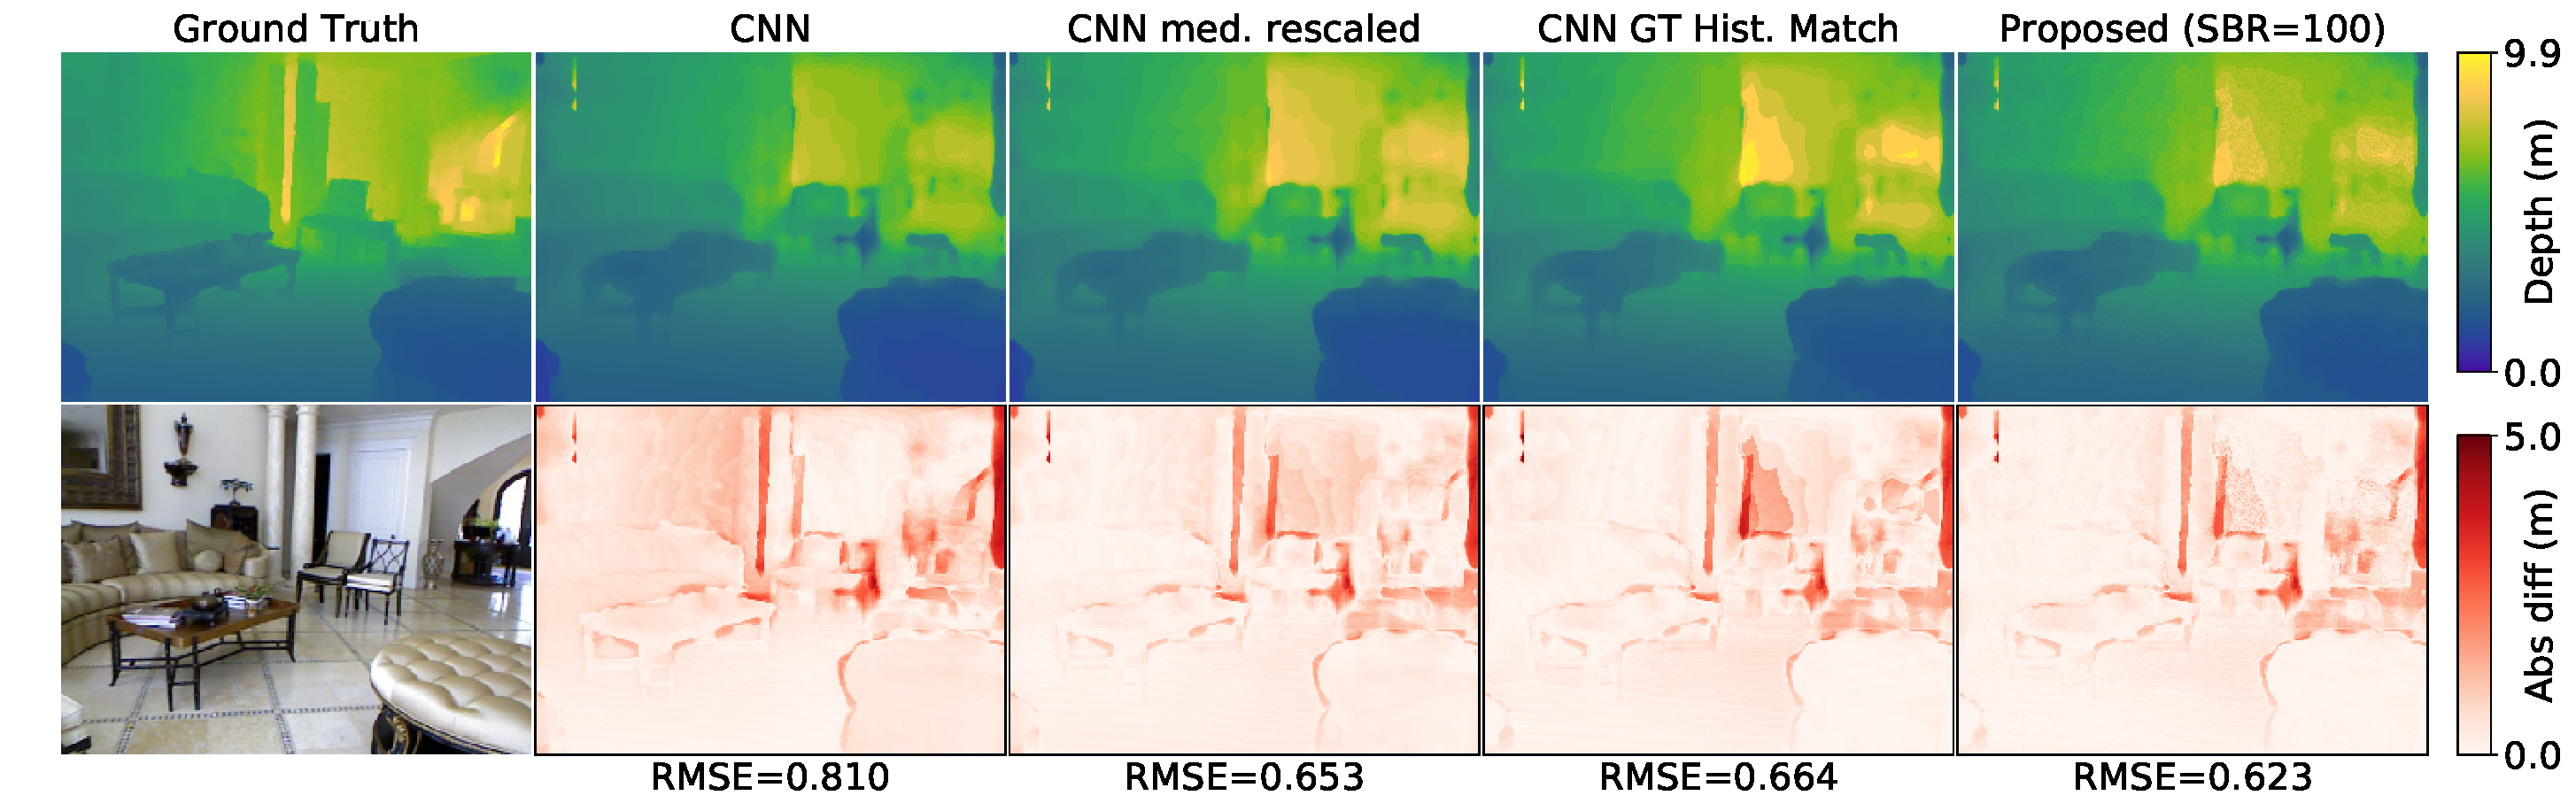
\includegraphics[width=\textwidth]{comparison/dorn_585_comparison.pdf}
%   \includegraphics[width=\textwidth]{comparison/dorn_633_comparison.pdf}
%   \includegraphics[width=\textwidth]{comparison/dorn_105_comparison.pdf}
%   \includegraphics[width=\textwidth]{comparison/dorn_220_comparison.pdf}
%   \caption{Results on DORN}
% \end{figure}
% \begin{figure}
%   \includegraphics[width=\textwidth]{comparison/dorn_252_comparison.pdf}
%   \includegraphics[width=\textwidth]{comparison/dorn_259_comparison.pdf}
%   \includegraphics[width=\textwidth]{comparison/dorn_178_comparison.pdf}
%   \includegraphics[width=\textwidth]{comparison/dorn_219_comparison.pdf}
%   \caption{Results on DORN}
% \end{figure}
% \begin{figure}
%   \includegraphics[width=\textwidth]{comparison/dorn_280_comparison.pdf}
%   \includegraphics[width=\textwidth]{comparison/dorn_293_comparison.pdf}
%   \includegraphics[width=\textwidth]{comparison/dorn_313_comparison.pdf}
%   \includegraphics[width=\textwidth]{comparison/dorn_413_comparison.pdf}
%   \caption{Results on DORN}
% \end{figure}
% \begin{figure}
  % \includegraphics[width=\textwidth]{comparison/dorn_477_comparison.pdf}
  % \includegraphics[width=\textwidth]{comparison/dorn_502_comparison.pdf}
%  \includegraphics[width=\textwidth]{comparison/dorn_428_comparison.pdf}
%  \includegraphics[width=\textwidth]{comparison/dorn_428_comparison.pdf}
  % \caption{Results on DORN}
% \end{figure}
% Densedepth:
% - Office: 18, 21
% - Bathroom: 25, 194, 285
% - Bookstore: 42
% - Kitchen: 52, 53, 103, 224, 226, 352, 362, 379
% - Office: 107, 187
% - Living Room: 140, 244, 527, 529
% - Dining Room: 219, 329, 346, 616
% - Bedroom: 390, 412, 420, 428, 457*, 468*, 477, 499
% Failure Cases: 258, 338(?), 341, 537 649 (minor)
% 
% DORN:
% - Office: 8, 14, 15, 23, 26
% - Living room: 63, 67, 140, 170, 522, 548, 569, 585, 633
% - Office: 105, 220, 252, 259* (interesting)
% - Kitchen: 178
% - Dining Room: 219
% - Bathroom: 280, 293, 313
% - Bedroom: 413, 477, 502
% 
% Failure Cases: 96, 266(?)



\section{Additional results for hardware prototype}
Figures \ref{fig:midas_captured_1}--\ref{fig:dorn_captured_3} show all the
captured results when the depth estimate is initialized with the MiDaS
\cite{Lasinger:2019} (Figures \ref{fig:midas_captured_1}--\ref{fig:midas_captured_3}),
DenseDepth (Figures \ref{fig:densedepth_captured_1}--\ref{fig:densedepth_captured_3}),
and DORN (Figures \ref{fig:dorn_captured_1}--\ref{fig:dorn_captured_3}). We compare
the output of the network $z_0$, the mean-rescaled network output where the
depth map $z_0$ has been scaled pixel-wise by the scalar
$\frac{\text{median}(h_{target})}{\text{median}(z_0)}$ ($h_{target}$ is the
processed SPAD transient), and the output of our method. As our laser is red, we
use the R channel of the RGB image as our reflectance map. We show absolute
difference maps and also give the root-mean-square-error (RMSE) for each
example.

Black pixels in the ground truth depth correspond to locations where our scanner
was unable to produce an accurate depth estimate (this can occur for a variety
of reasons including dark albedo and surface specularity). These pixels are masked off and not used in the RMSE
calculation, and appear as an absolute difference of 0 in the difference maps.
 \begin{figure}[H]
    \centering
    \begin{tabular}{p{5mm}*{4}{>{\centering\arraybackslash}p{1.15in}}c}
      \multirow[t]{5}{=}[-1in]{\rotatebox[origin=rc]{90}{Kitchen Scene}} & Ground Truth & CNN & CNN Mean Rescaled & CNN Histogram Matched & \\
      &
      \includegraphics[height=1.15in, width=1.15in]{captured/midas/8_29_kitchen_scene/gt_z_proj_crop_depth_fig.png}&
      \includegraphics[height=1.15in, width=1.15in]{captured/midas/8_29_kitchen_scene/z_init_depth_fig.png}&
      \includegraphics[height=1.15in, width=1.15in]{captured/midas/8_29_kitchen_scene/z_med_scaled_depth_fig.png}&
      \includegraphics[height=1.15in, width=1.15in]{captured/midas/8_29_kitchen_scene/z_pred_depth_fig.png}&
      \includegraphics[height=1.15in]{captured/midas/8_29_kitchen_scene/depth_colorbar.pdf}\\
%      & RGB &  &  &  & \\
      &
      \includegraphics[height=1.15in, width=1.15in]{captured/midas/8_29_kitchen_scene/rgb_cropped_fig.png}&
      \includegraphics[height=1.15in, width=1.15in]{captured/midas/8_29_kitchen_scene/z_init_diff_fig.png}&
      \includegraphics[height=1.15in, width=1.15in]{captured/midas/8_29_kitchen_scene/z_med_scaled_diff_fig.png}&
      \includegraphics[height=1.15in, width=1.15in]{captured/midas/8_29_kitchen_scene/z_pred_diff_fig.png}&
      \includegraphics[height=1.15in]{captured/midas/8_29_kitchen_scene/diff_colorbar.pdf}\\
      & RGB & RMSE = 2.914 & RMSE = 1.441 & RMSE = 0.606& \\ 

      \rule{0pt}{3ex}  & & & & & \\
      \multirow[t]{3}{=}{\rotatebox[origin=c]{90}{Conference Room 1}}& 
      \includegraphics[height=1.15in, width=1.15in]{captured/midas/8_29_conference_room_scene/gt_z_proj_crop_depth_fig.png}&
      \includegraphics[height=1.15in, width=1.15in]{captured/midas/8_29_conference_room_scene/z_init_depth_fig.png}&
      \includegraphics[height=1.15in, width=1.15in]{captured/midas/8_29_conference_room_scene/z_med_scaled_depth_fig.png}&
      \includegraphics[height=1.15in, width=1.15in]{captured/midas/8_29_conference_room_scene/z_pred_depth_fig.png}&
      \includegraphics[height=1.15in]{captured/midas/8_29_conference_room_scene/depth_colorbar.pdf}\\

      &
      \includegraphics[height=1.15in, width=1.15in]{captured/midas/8_29_conference_room_scene/rgb_cropped_fig.png}&
      \includegraphics[height=1.15in, width=1.15in]{captured/midas/8_29_conference_room_scene/z_init_diff_fig.png}&
      \includegraphics[height=1.15in, width=1.15in]{captured/midas/8_29_conference_room_scene/z_med_scaled_diff_fig.png}&
      \includegraphics[height=1.15in, width=1.15in]{captured/midas/8_29_conference_room_scene/z_pred_diff_fig.png}&
      \includegraphics[height=1.15in]{captured/midas/8_29_conference_room_scene/diff_colorbar.pdf}\\
      & & RMSE = 2.914 & RMSE = 1.441 & RMSE = 0.606& \\ 

      \rule{0pt}{3ex}  & & & & & \\
      \multirow[t]{3}{=}{\rotatebox[origin=c]{90}{Conference Room 2}}&
      \includegraphics[height=1.15in, width=1.15in]{captured/midas/8_30_conference_room2_scene/gt_z_proj_crop_depth_fig.png}&
      \includegraphics[height=1.15in, width=1.15in]{captured/midas/8_30_conference_room2_scene/z_init_depth_fig.png}&
      \includegraphics[height=1.15in, width=1.15in]{captured/midas/8_30_conference_room2_scene/z_med_scaled_depth_fig.png}&
      \includegraphics[height=1.15in, width=1.15in]{captured/midas/8_30_conference_room2_scene/z_pred_depth_fig.png}&
      \includegraphics[height=1.15in]{captured/midas/8_30_conference_room2_scene/depth_colorbar.pdf}\\

      &
      \includegraphics[height=1.15in, width=1.15in]{captured/midas/8_30_conference_room2_scene/rgb_cropped_fig.png}&
      \includegraphics[height=1.15in, width=1.15in]{captured/midas/8_30_conference_room2_scene/z_init_diff_fig.png}&
      \includegraphics[height=1.15in, width=1.15in]{captured/midas/8_30_conference_room2_scene/z_med_scaled_diff_fig.png}&
      \includegraphics[height=1.15in, width=1.15in]{captured/midas/8_30_conference_room2_scene/z_pred_diff_fig.png}&
      \includegraphics[height=1.15in]{captured/midas/8_30_conference_room2_scene/diff_colorbar.pdf}\\
      & & RMSE = 2.914 & RMSE = 1.441 & RMSE = 0.606& \\ 
    \end{tabular}
    \caption{Captured results initialized using the MiDaS CNN.
      Second row shows absolute difference between above estimates and ground
      truth. MiDaS does not output metric depth, so the CNN depth maps are
      scaled to be in the range $(0.494, 9.094)$ by default. However, MiDaS does produce
      accurate ordinal depth, leading to stronger performance of our histogram
      matching compared to other methods.}
    \label{fig:midas_captured_1}
%    \vspace{-1.5em}
\end{figure}
\begin{figure}[H]
    \centering
    \begin{tabular}{p{5mm}*{4}{>{\centering\arraybackslash}p{1.15in}}c}
      \multirow[t]{5}{=}[-1in]{\rotatebox[origin=rc]{90}{Hallway}} & Ground Truth & CNN & CNN Mean Rescaled & CNN Histogram Matched & \\
      &
      \includegraphics[width=1.15in, height=1.15in]{captured/midas/8_30_Hallway/gt_z_proj_crop_depth_fig.png}&
      \includegraphics[width=1.15in, height=1.15in]{captured/midas/8_30_Hallway/z_init_depth_fig.png}&
      \includegraphics[width=1.15in, height=1.15in]{captured/midas/8_30_Hallway/z_med_scaled_depth_fig.png}&
      \includegraphics[width=1.15in, height=1.15in]{captured/midas/8_30_Hallway/z_pred_depth_fig.png}&
      \includegraphics[height=1.15in]{captured/midas/8_30_Hallway/depth_colorbar.pdf}\\
      & & & & & \\

      & 
      \includegraphics[width=1.15in, height=1.15in]{captured/midas/8_30_Hallway/rgb_cropped_fig.png}&
      \includegraphics[width=1.15in, height=1.15in]{captured/midas/8_30_Hallway/z_init_diff_fig.png}&
      \includegraphics[width=1.15in, height=1.15in]{captured/midas/8_30_Hallway/z_med_scaled_diff_fig.png}&
      \includegraphics[width=1.15in, height=1.15in]{captured/midas/8_30_Hallway/z_pred_diff_fig.png}&
      \includegraphics[height=1.15in]{captured/midas/8_30_Hallway/diff_colorbar.pdf}\\
      & RGB & RMSE = 2.914 & RMSE = 1.441 & RMSE = 0.606& \\ 

      \rule{0pt}{3ex}  & & & & & \\
      \multirow[t]{3}{=}{\rotatebox[origin=c]{90}{Poster}}&
      \includegraphics[width=1.15in, height=1.15in]{captured/midas/8_30_poster_scene/gt_z_proj_crop_depth_fig.png}&
      \includegraphics[width=1.15in, height=1.15in]{captured/midas/8_30_poster_scene/z_init_depth_fig.png}&
      \includegraphics[width=1.15in, height=1.15in]{captured/midas/8_30_poster_scene/z_med_scaled_depth_fig.png}&
      \includegraphics[width=1.15in, height=1.15in]{captured/midas/8_30_poster_scene/z_pred_depth_fig.png}&
      \includegraphics[height=1.15in]{captured/midas/8_30_poster_scene/depth_colorbar.pdf}\\

      &
      \includegraphics[width=1.15in, height=1.15in]{captured/midas/8_30_poster_scene/rgb_cropped_fig.png}&
      \includegraphics[width=1.15in, height=1.15in]{captured/midas/8_30_poster_scene/z_init_diff_fig.png}&
      \includegraphics[width=1.15in, height=1.15in]{captured/midas/8_30_poster_scene/z_med_scaled_diff_fig.png}&
      \includegraphics[width=1.15in, height=1.15in]{captured/midas/8_30_poster_scene/z_pred_diff_fig.png}&
      \includegraphics[height=1.15in]{captured/midas/8_30_poster_scene/diff_colorbar.pdf}\\
      & & RMSE = 2.914 & RMSE = 1.441 & RMSE = 0.606& \\ 

      \rule{0pt}{3ex}  & & & & & \\
      \multirow[t]{3}{=}{\rotatebox[origin=c]{90}{Bookshelf}}&
      \includegraphics[width=1.15in, height=1.15in]{captured/midas/8_30_small_lab_scene/gt_z_proj_crop_depth_fig.png}&
      \includegraphics[width=1.15in, height=1.15in]{captured/midas/8_30_small_lab_scene/z_init_depth_fig.png}&
      \includegraphics[width=1.15in, height=1.15in]{captured/midas/8_30_small_lab_scene/z_med_scaled_depth_fig.png}&
      \includegraphics[width=1.15in, height=1.15in]{captured/midas/8_30_small_lab_scene/z_pred_depth_fig.png}&
      \includegraphics[height=1.15in]{captured/midas/8_30_small_lab_scene/depth_colorbar.pdf}\\

      &
      \includegraphics[width=1.15in, height=1.15in]{captured/midas/8_30_small_lab_scene/rgb_cropped_fig.png}&
      \includegraphics[width=1.15in, height=1.15in]{captured/midas/8_30_small_lab_scene/z_init_diff_fig.png}&
      \includegraphics[width=1.15in, height=1.15in]{captured/midas/8_30_small_lab_scene/z_med_scaled_diff_fig.png}&
      \includegraphics[width=1.15in, height=1.15in]{captured/midas/8_30_small_lab_scene/z_pred_diff_fig.png}&
      \includegraphics[height=1.15in]{captured/midas/8_30_small_lab_scene/diff_colorbar.pdf}\\
      & & RMSE = 2.914 & RMSE = 1.441 & RMSE = 0.606\\ 
                                     
%      (a)&(b)&(c)&(d)&(e)\\
    \end{tabular}
    \vspace{-1em}
    \caption{Captured results initialized using the MiDaS CNN.
      Second row shows absolute difference between above estimates and ground
      truth.MiDaS does not output metric depth, so the CNN depth maps are
      scaled to be in the range $(0.494, 9.094)$ by default. However, MiDaS does produce
      accurate ordinal depth, leading to stronger performance of our histogram
      matching compared to other methods.}
    \label{fig:midas_captured_2}
%    \vspace{-1.5em}
\end{figure}
 
% %% MiDaS outdoor scene
\begin{figure}[H]
    \centering
    \begin{tabular}{p{5mm}*{4}{>{\centering\arraybackslash}p{1.15in}}c}
      \multirow[t]{5}{=}[-1in]{\rotatebox[origin=rc]{90}{Outdoor Scene}} & Ground Truth & CNN & CNN Mean Rescaled & CNN Histogram Matched & \\
      &
      \includegraphics[height=1.15in, width=1.15in]{captured/midas/8_31_outdoor3/gt_z_proj_crop_depth_fig.png}&
      \includegraphics[height=1.15in, width=1.15in]{captured/midas/8_31_outdoor3/z_init_depth_fig.png}&
      \includegraphics[height=1.15in, width=1.15in]{captured/midas/8_31_outdoor3/z_med_scaled_depth_fig.png}&
      \includegraphics[height=1.15in, width=1.15in]{captured/midas/8_31_outdoor3/z_pred_depth_fig.png}&
      \includegraphics[height=1.15in]{captured/midas/8_31_outdoor3/depth_colorbar.pdf}\\
%      & RGB &  &  &  & \\
      &
      \includegraphics[height=1.15in, width=1.15in]{captured/midas/8_31_outdoor3/rgb_cropped_fig.png}&
      \includegraphics[height=1.15in, width=1.15in]{captured/midas/8_31_outdoor3/z_init_diff_fig.png}&
      \includegraphics[height=1.15in, width=1.15in]{captured/midas/8_31_outdoor3/z_med_scaled_diff_fig.png}&
      \includegraphics[height=1.15in, width=1.15in]{captured/midas/8_31_outdoor3/z_pred_diff_fig.png}&
      \includegraphics[height=1.15in]{captured/midas/8_31_outdoor3/diff_colorbar.pdf}\\
      & RGB & RMSE = 2.914 & RMSE = 1.441 & RMSE = 0.606& \\ 
    \end{tabular}
    \caption{Captured results initialized using the MiDaS CNN on an outdoor scene.
      Second row shows absolute difference between above estimates and ground
      truth. MiDaS does not output metric depth, so the CNN depth map is
      scaled to be in the range $(0.494, 11.094)$ by default. However, MiDaS does produce
      accurate ordinal depth, leading to stronger performance of our histogram
      matching compared to other methods.
}
    \label{fig:midas_captured_3}
%    \vspace{-1.5em}
\end{figure}


\begin{figure}[H]
    \centering
    \begin{tabular}{p{5mm}*{4}{>{\centering\arraybackslash}p{1.15in}}c}
      \multirow[t]{5}{=}[-1in]{\rotatebox[origin=rc]{90}{Kitchen Scene}} & Ground Truth & CNN & CNN Mean Rescaled & CNN Histogram Matched & \\
      &
      \includegraphics[height=1.15in, width=1.15in]{captured/densedepth/8_29_kitchen_scene/gt_z_proj_crop_depth_fig.png}&
      \includegraphics[height=1.15in, width=1.15in]{captured/densedepth/8_29_kitchen_scene/z_init_depth_fig.png}&
      \includegraphics[height=1.15in, width=1.15in]{captured/densedepth/8_29_kitchen_scene/z_med_scaled_depth_fig.png}&
      \includegraphics[height=1.15in, width=1.15in]{captured/densedepth/8_29_kitchen_scene/z_pred_depth_fig.png}&
      \includegraphics[height=1.15in]{captured/densedepth/8_29_kitchen_scene/depth_colorbar.pdf}\\
%      & RGB &  &  &  & \\
      &
      \includegraphics[height=1.15in, width=1.15in]{captured/densedepth/8_29_kitchen_scene/rgb_cropped_fig.png}&
      \includegraphics[height=1.15in, width=1.15in]{captured/densedepth/8_29_kitchen_scene/z_init_diff_fig.png}&
      \includegraphics[height=1.15in, width=1.15in]{captured/densedepth/8_29_kitchen_scene/z_med_scaled_diff_fig.png}&
      \includegraphics[height=1.15in, width=1.15in]{captured/densedepth/8_29_kitchen_scene/z_pred_diff_fig.png}&
      \includegraphics[height=1.15in]{captured/densedepth/8_29_kitchen_scene/diff_colorbar.pdf}\\
      & RGB & RMSE = 2.914 & RMSE = 1.441 & RMSE = 0.606& \\ 

      \rule{0pt}{3ex}  & & & & & \\
      \multirow[t]{3}{=}{\rotatebox[origin=c]{90}{Conference Room 1}}& 
      \includegraphics[height=1.15in, width=1.15in]{captured/densedepth/8_29_conference_room_scene/gt_z_proj_crop_depth_fig.png}&
      \includegraphics[height=1.15in, width=1.15in]{captured/densedepth/8_29_conference_room_scene/z_init_depth_fig.png}&
      \includegraphics[height=1.15in, width=1.15in]{captured/densedepth/8_29_conference_room_scene/z_med_scaled_depth_fig.png}&
      \includegraphics[height=1.15in, width=1.15in]{captured/densedepth/8_29_conference_room_scene/z_pred_depth_fig.png}&
      \includegraphics[height=1.15in]{captured/densedepth/8_29_conference_room_scene/depth_colorbar.pdf}\\

      &
      \includegraphics[height=1.15in, width=1.15in]{captured/densedepth/8_29_conference_room_scene/rgb_cropped_fig.png}&
      \includegraphics[height=1.15in, width=1.15in]{captured/densedepth/8_29_conference_room_scene/z_init_diff_fig.png}&
      \includegraphics[height=1.15in, width=1.15in]{captured/densedepth/8_29_conference_room_scene/z_med_scaled_diff_fig.png}&
      \includegraphics[height=1.15in, width=1.15in]{captured/densedepth/8_29_conference_room_scene/z_pred_diff_fig.png}&
      \includegraphics[height=1.15in]{captured/densedepth/8_29_conference_room_scene/diff_colorbar.pdf}\\
      & & RMSE = 2.914 & RMSE = 1.441 & RMSE = 0.606& \\ 

      \rule{0pt}{3ex}  & & & & & \\
      \multirow[t]{3}{=}{\rotatebox[origin=c]{90}{Conference Room 2}}&
      \includegraphics[height=1.15in, width=1.15in]{captured/densedepth/8_30_conference_room2_scene/gt_z_proj_crop_depth_fig.png}&
      \includegraphics[height=1.15in, width=1.15in]{captured/densedepth/8_30_conference_room2_scene/z_init_depth_fig.png}&
      \includegraphics[height=1.15in, width=1.15in]{captured/densedepth/8_30_conference_room2_scene/z_med_scaled_depth_fig.png}&
      \includegraphics[height=1.15in, width=1.15in]{captured/densedepth/8_30_conference_room2_scene/z_pred_depth_fig.png}&
      \includegraphics[height=1.15in]{captured/densedepth/8_30_conference_room2_scene/depth_colorbar.pdf}\\

      &
      \includegraphics[height=1.15in, width=1.15in]{captured/densedepth/8_30_conference_room2_scene/rgb_cropped_fig.png}&
      \includegraphics[height=1.15in, width=1.15in]{captured/densedepth/8_30_conference_room2_scene/z_init_diff_fig.png}&
      \includegraphics[height=1.15in, width=1.15in]{captured/densedepth/8_30_conference_room2_scene/z_med_scaled_diff_fig.png}&
      \includegraphics[height=1.15in, width=1.15in]{captured/densedepth/8_30_conference_room2_scene/z_pred_diff_fig.png}&
      \includegraphics[height=1.15in]{captured/densedepth/8_30_conference_room2_scene/diff_colorbar.pdf}\\
      & & RMSE = 2.914 & RMSE = 1.441 & RMSE = 0.606& \\ 
    \end{tabular}
    \caption{Captured results initialized using the DenseDepth CNN.
      Second row shows absolute difference between above estimates and ground truth.}
    \label{fig:densedepth_captured_1}
%    \vspace{-1.5em}
\end{figure}
\begin{figure}[H]
    \centering
    \begin{tabular}{p{5mm}*{4}{>{\centering\arraybackslash}p{1.15in}}c}
      \multirow[t]{5}{=}[-1in]{\rotatebox[origin=rc]{90}{Hallway}} & Ground Truth & CNN & CNN Mean Rescaled & CNN Histogram Matched & \\
      &
      \includegraphics[width=1.15in, height=1.15in]{captured/densedepth/8_30_Hallway/gt_z_proj_crop_depth_fig.png}&
      \includegraphics[width=1.15in, height=1.15in]{captured/densedepth/8_30_Hallway/z_init_depth_fig.png}&
      \includegraphics[width=1.15in, height=1.15in]{captured/densedepth/8_30_Hallway/z_med_scaled_depth_fig.png}&
      \includegraphics[width=1.15in, height=1.15in]{captured/densedepth/8_30_Hallway/z_pred_depth_fig.png}&
      \includegraphics[height=1.15in]{captured/densedepth/8_30_Hallway/depth_colorbar.pdf}\\
      & & & & & \\

      & 
      \includegraphics[width=1.15in, height=1.15in]{captured/densedepth/8_30_Hallway/rgb_cropped_fig.png}&
      \includegraphics[width=1.15in, height=1.15in]{captured/densedepth/8_30_Hallway/z_init_diff_fig.png}&
      \includegraphics[width=1.15in, height=1.15in]{captured/densedepth/8_30_Hallway/z_med_scaled_diff_fig.png}&
      \includegraphics[width=1.15in, height=1.15in]{captured/densedepth/8_30_Hallway/z_pred_diff_fig.png}&
      \includegraphics[height=1.15in]{captured/densedepth/8_30_Hallway/diff_colorbar.pdf}\\
      & RGB & RMSE = 2.914 & RMSE = 1.441 & RMSE = 0.606& \\ 

      \rule{0pt}{3ex}  & & & & & \\
      \multirow[t]{3}{=}{\rotatebox[origin=c]{90}{Poster}}&
      \includegraphics[width=1.15in, height=1.15in]{captured/densedepth/8_30_poster_scene/gt_z_proj_crop_depth_fig.png}&
      \includegraphics[width=1.15in, height=1.15in]{captured/densedepth/8_30_poster_scene/z_init_depth_fig.png}&
      \includegraphics[width=1.15in, height=1.15in]{captured/densedepth/8_30_poster_scene/z_med_scaled_depth_fig.png}&
      \includegraphics[width=1.15in, height=1.15in]{captured/densedepth/8_30_poster_scene/z_pred_depth_fig.png}&
      \includegraphics[height=1.15in]{captured/densedepth/8_30_poster_scene/depth_colorbar.pdf}\\

      &
      \includegraphics[width=1.15in, height=1.15in]{captured/densedepth/8_30_poster_scene/rgb_cropped_fig.png}&
      \includegraphics[width=1.15in, height=1.15in]{captured/densedepth/8_30_poster_scene/z_init_diff_fig.png}&
      \includegraphics[width=1.15in, height=1.15in]{captured/densedepth/8_30_poster_scene/z_med_scaled_diff_fig.png}&
      \includegraphics[width=1.15in, height=1.15in]{captured/densedepth/8_30_poster_scene/z_pred_diff_fig.png}&
      \includegraphics[height=1.15in]{captured/densedepth/8_30_poster_scene/diff_colorbar.pdf}\\
      & & RMSE = 2.914 & RMSE = 1.441 & RMSE = 0.606& \\ 

      \rule{0pt}{3ex}  & & & & & \\
      \multirow[t]{3}{=}{\rotatebox[origin=c]{90}{Bookshelf}}&
      \includegraphics[width=1.15in, height=1.15in]{captured/densedepth/8_30_small_lab_scene/gt_z_proj_crop_depth_fig.png}&
      \includegraphics[width=1.15in, height=1.15in]{captured/densedepth/8_30_small_lab_scene/z_init_depth_fig.png}&
      \includegraphics[width=1.15in, height=1.15in]{captured/densedepth/8_30_small_lab_scene/z_med_scaled_depth_fig.png}&
      \includegraphics[width=1.15in, height=1.15in]{captured/densedepth/8_30_small_lab_scene/z_pred_depth_fig.png}&
      \includegraphics[height=1.15in]{captured/densedepth/8_30_small_lab_scene/depth_colorbar.pdf}\\

      &
      \includegraphics[width=1.15in, height=1.15in]{captured/densedepth/8_30_small_lab_scene/rgb_cropped_fig.png}&
      \includegraphics[width=1.15in, height=1.15in]{captured/densedepth/8_30_small_lab_scene/z_init_diff_fig.png}&
      \includegraphics[width=1.15in, height=1.15in]{captured/densedepth/8_30_small_lab_scene/z_med_scaled_diff_fig.png}&
      \includegraphics[width=1.15in, height=1.15in]{captured/densedepth/8_30_small_lab_scene/z_pred_diff_fig.png}&
      \includegraphics[height=1.15in]{captured/densedepth/8_30_small_lab_scene/diff_colorbar.pdf}\\
      & & RMSE = 2.914 & RMSE = 1.441 & RMSE = 0.606\\ 
                                     
%      (a)&(b)&(c)&(d)&(e)\\
    \end{tabular}
    \caption{Captured results initialized using the DenseDepth CNN.
      Second row shows absolute difference between above estimates and ground truth.}
    \label{fig:densedepth_captured_2}
%    \vspace{-1.5em}
\end{figure}
%% DenseDepth outdoor scene
\begin{figure}[H]
    \centering
    \begin{tabular}{p{5mm}*{4}{>{\centering\arraybackslash}p{1.15in}}c}
      \multirow[t]{5}{=}[-1in]{\rotatebox[origin=rc]{90}{Outdoor Scene}} & Ground Truth & CNN & CNN Mean Rescaled & CNN Histogram Matched & \\
      &
      \includegraphics[height=1.15in, width=1.15in]{captured/densedepth/8_31_outdoor3/gt_z_proj_crop_depth_fig.png}&
      \includegraphics[height=1.15in, width=1.15in]{captured/densedepth/8_31_outdoor3/z_init_depth_fig.png}&
      \includegraphics[height=1.15in, width=1.15in]{captured/densedepth/8_31_outdoor3/z_med_scaled_depth_fig.png}&
      \includegraphics[height=1.15in, width=1.15in]{captured/densedepth/8_31_outdoor3/z_pred_depth_fig.png}&
      \includegraphics[height=1.15in]{captured/densedepth/8_31_outdoor3/depth_colorbar.pdf}\\
%      & RGB &  &  &  & \\
      &
      \includegraphics[height=1.15in, width=1.15in]{captured/densedepth/8_31_outdoor3/rgb_cropped_fig.png}&
      \includegraphics[height=1.15in, width=1.15in]{captured/densedepth/8_31_outdoor3/z_init_diff_fig.png}&
      \includegraphics[height=1.15in, width=1.15in]{captured/densedepth/8_31_outdoor3/z_med_scaled_diff_fig.png}&
      \includegraphics[height=1.15in, width=1.15in]{captured/densedepth/8_31_outdoor3/z_pred_diff_fig.png}&
      \includegraphics[height=1.15in]{captured/densedepth/8_31_outdoor3/diff_colorbar.pdf}\\
      & RGB & RMSE = 2.914 & RMSE = 1.441 & RMSE = 0.606& \\ 
    \end{tabular}
    \caption{Captured results initialized using the DenseDepth CNN on an outdoor scene.
      Second row shows absolute difference between above estimates and ground truth.}
    \label{fig:densedepth_captured_3}
%    \vspace{-1.5em}
\end{figure}


% %%%%%%%%%%%%%%%%%%%%%%%%%%%%%%%%%%%%%%%
 
\begin{figure}[H]
    \centering
    \begin{tabular}{p{5mm}*{4}{>{\centering\arraybackslash}p{1.15in}}c}
      \multirow[t]{5}{=}[-1in]{\rotatebox[origin=rc]{90}{Kitchen Scene}} & Ground Truth & CNN & CNN Mean Rescaled & CNN Histogram Matched & \\
      &
      \includegraphics[height=1.15in, width=1.15in]{captured/dorn/8_29_kitchen_scene/gt_z_proj_crop_depth_fig.png}&
      \includegraphics[height=1.15in, width=1.15in]{captured/dorn/8_29_kitchen_scene/z_init_depth_fig.png}&
      \includegraphics[height=1.15in, width=1.15in]{captured/dorn/8_29_kitchen_scene/z_med_scaled_depth_fig.png}&
      \includegraphics[height=1.15in, width=1.15in]{captured/dorn/8_29_kitchen_scene/z_pred_depth_fig.png}&
      \includegraphics[height=1.15in]{captured/dorn/8_29_kitchen_scene/depth_colorbar.pdf}\\
%      & RGB &  &  &  & \\
      &
      \includegraphics[height=1.15in, width=1.15in]{captured/dorn/8_29_kitchen_scene/rgb_cropped_fig.png}&
      \includegraphics[height=1.15in, width=1.15in]{captured/dorn/8_29_kitchen_scene/z_init_diff_fig.png}&
      \includegraphics[height=1.15in, width=1.15in]{captured/dorn/8_29_kitchen_scene/z_med_scaled_diff_fig.png}&
      \includegraphics[height=1.15in, width=1.15in]{captured/dorn/8_29_kitchen_scene/z_pred_diff_fig.png}&
      \includegraphics[height=1.15in]{captured/dorn/8_29_kitchen_scene/diff_colorbar.pdf}\\
      & RGB & RMSE = 2.914 & RMSE = 1.441 & RMSE = 0.606& \\ 

      \rule{0pt}{3ex}  & & & & & \\
      \multirow[t]{3}{=}{\rotatebox[origin=c]{90}{Conference Room 1}}& 
      \includegraphics[height=1.15in, width=1.15in]{captured/dorn/8_29_conference_room_scene/gt_z_proj_crop_depth_fig.png}&
      \includegraphics[height=1.15in, width=1.15in]{captured/dorn/8_29_conference_room_scene/z_init_depth_fig.png}&
      \includegraphics[height=1.15in, width=1.15in]{captured/dorn/8_29_conference_room_scene/z_med_scaled_depth_fig.png}&
      \includegraphics[height=1.15in, width=1.15in]{captured/dorn/8_29_conference_room_scene/z_pred_depth_fig.png}&
      \includegraphics[height=1.15in]{captured/dorn/8_29_conference_room_scene/depth_colorbar.pdf}\\

      &
      \includegraphics[height=1.15in, width=1.15in]{captured/dorn/8_29_conference_room_scene/rgb_cropped_fig.png}&
      \includegraphics[height=1.15in, width=1.15in]{captured/dorn/8_29_conference_room_scene/z_init_diff_fig.png}&
      \includegraphics[height=1.15in, width=1.15in]{captured/dorn/8_29_conference_room_scene/z_med_scaled_diff_fig.png}&
      \includegraphics[height=1.15in, width=1.15in]{captured/dorn/8_29_conference_room_scene/z_pred_diff_fig.png}&
      \includegraphics[height=1.15in]{captured/dorn/8_29_conference_room_scene/diff_colorbar.pdf}\\
      & & RMSE = 2.914 & RMSE = 1.441 & RMSE = 0.606& \\ 

      \rule{0pt}{3ex}  & & & & & \\
      \multirow[t]{3}{=}{\rotatebox[origin=c]{90}{Conference Room 2}}&
      \includegraphics[height=1.15in, width=1.15in]{captured/dorn/8_30_conference_room2_scene/gt_z_proj_crop_depth_fig.png}&
      \includegraphics[height=1.15in, width=1.15in]{captured/dorn/8_30_conference_room2_scene/z_init_depth_fig.png}&
      \includegraphics[height=1.15in, width=1.15in]{captured/dorn/8_30_conference_room2_scene/z_med_scaled_depth_fig.png}&
      \includegraphics[height=1.15in, width=1.15in]{captured/dorn/8_30_conference_room2_scene/z_pred_depth_fig.png}&
      \includegraphics[height=1.15in]{captured/dorn/8_30_conference_room2_scene/depth_colorbar.pdf}\\

      &
      \includegraphics[height=1.15in, width=1.15in]{captured/dorn/8_30_conference_room2_scene/rgb_cropped_fig.png}&
      \includegraphics[height=1.15in, width=1.15in]{captured/dorn/8_30_conference_room2_scene/z_init_diff_fig.png}&
      \includegraphics[height=1.15in, width=1.15in]{captured/dorn/8_30_conference_room2_scene/z_med_scaled_diff_fig.png}&
      \includegraphics[height=1.15in, width=1.15in]{captured/dorn/8_30_conference_room2_scene/z_pred_diff_fig.png}&
      \includegraphics[height=1.15in]{captured/dorn/8_30_conference_room2_scene/diff_colorbar.pdf}\\
      & & RMSE = 2.914 & RMSE = 1.441 & RMSE = 0.606& \\ 
    \end{tabular}
    \caption{Captured results initialized using the DORN CNN.
      Second row shows absolute difference between above estimates and ground truth.}
    \label{fig:dorn_captured_1}
%    \vspace{-1.5em}
\end{figure}

\begin{figure}[H]
    \centering
    \begin{tabular}{p{5mm}*{4}{>{\centering\arraybackslash}p{1.15in}}c}
      \multirow[t]{5}{=}[-1in]{\rotatebox[origin=rc]{90}{Hallway}} & Ground Truth & CNN & CNN Mean Rescaled & CNN Histogram Matched & \\
      &
      \includegraphics[width=1.15in, height=1.15in]{captured/dorn/8_30_Hallway/gt_z_proj_crop_depth_fig.png}&
      \includegraphics[width=1.15in, height=1.15in]{captured/dorn/8_30_Hallway/z_init_depth_fig.png}&
      \includegraphics[width=1.15in, height=1.15in]{captured/dorn/8_30_Hallway/z_med_scaled_depth_fig.png}&
      \includegraphics[width=1.15in, height=1.15in]{captured/dorn/8_30_Hallway/z_pred_depth_fig.png}&
      \includegraphics[height=1.15in]{captured/dorn/8_30_Hallway/depth_colorbar.pdf}\\
      & & & & & \\

      & 
      \includegraphics[width=1.15in, height=1.15in]{captured/dorn/8_30_Hallway/rgb_cropped_fig.png}&
      \includegraphics[width=1.15in, height=1.15in]{captured/dorn/8_30_Hallway/z_init_diff_fig.png}&
      \includegraphics[width=1.15in, height=1.15in]{captured/dorn/8_30_Hallway/z_med_scaled_diff_fig.png}&
      \includegraphics[width=1.15in, height=1.15in]{captured/dorn/8_30_Hallway/z_pred_diff_fig.png}&
      \includegraphics[height=1.15in]{captured/dorn/8_30_Hallway/diff_colorbar.pdf}\\
      & RGB & RMSE = 2.914 & RMSE = 1.441 & RMSE = 0.606& \\ 

      \rule{0pt}{3ex}  & & & & & \\
      \multirow[t]{3}{=}{\rotatebox[origin=c]{90}{Poster}}&
      \includegraphics[width=1.15in, height=1.15in]{captured/dorn/8_30_poster_scene/gt_z_proj_crop_depth_fig.png}&
      \includegraphics[width=1.15in, height=1.15in]{captured/dorn/8_30_poster_scene/z_init_depth_fig.png}&
      \includegraphics[width=1.15in, height=1.15in]{captured/dorn/8_30_poster_scene/z_med_scaled_depth_fig.png}&
      \includegraphics[width=1.15in, height=1.15in]{captured/dorn/8_30_poster_scene/z_pred_depth_fig.png}&
      \includegraphics[height=1.15in]{captured/dorn/8_30_poster_scene/depth_colorbar.pdf}\\

      &
      \includegraphics[width=1.15in, height=1.15in]{captured/dorn/8_30_poster_scene/rgb_cropped_fig.png}&
      \includegraphics[width=1.15in, height=1.15in]{captured/dorn/8_30_poster_scene/z_init_diff_fig.png}&
      \includegraphics[width=1.15in, height=1.15in]{captured/dorn/8_30_poster_scene/z_med_scaled_diff_fig.png}&
      \includegraphics[width=1.15in, height=1.15in]{captured/dorn/8_30_poster_scene/z_pred_diff_fig.png}&
      \includegraphics[height=1.15in]{captured/dorn/8_30_poster_scene/diff_colorbar.pdf}\\
      & & RMSE = 2.914 & RMSE = 1.441 & RMSE = 0.606& \\ 

      \rule{0pt}{3ex}  & & & & & \\
      \multirow[t]{3}{=}{\rotatebox[origin=c]{90}{Bookshelf}}&
      \includegraphics[width=1.15in, height=1.15in]{captured/dorn/8_30_small_lab_scene/gt_z_proj_crop_depth_fig.png}&
      \includegraphics[width=1.15in, height=1.15in]{captured/dorn/8_30_small_lab_scene/z_init_depth_fig.png}&
      \includegraphics[width=1.15in, height=1.15in]{captured/dorn/8_30_small_lab_scene/z_med_scaled_depth_fig.png}&
      \includegraphics[width=1.15in, height=1.15in]{captured/dorn/8_30_small_lab_scene/z_pred_depth_fig.png}&
      \includegraphics[height=1.15in]{captured/dorn/8_30_small_lab_scene/depth_colorbar.pdf}\\

      &
      \includegraphics[width=1.15in, height=1.15in]{captured/dorn/8_30_small_lab_scene/rgb_cropped_fig.png}&
      \includegraphics[width=1.15in, height=1.15in]{captured/dorn/8_30_small_lab_scene/z_init_diff_fig.png}&
      \includegraphics[width=1.15in, height=1.15in]{captured/dorn/8_30_small_lab_scene/z_med_scaled_diff_fig.png}&
      \includegraphics[width=1.15in, height=1.15in]{captured/dorn/8_30_small_lab_scene/z_pred_diff_fig.png}&
      \includegraphics[height=1.15in]{captured/dorn/8_30_small_lab_scene/diff_colorbar.pdf}\\
      & & RMSE = 2.914 & RMSE = 1.441 & RMSE = 0.606\\ 
                                     
%      (a)&(b)&(c)&(d)&(e)\\
    \end{tabular}
    \caption{Captured results initialized using the DORN CNN.
      Second row shows absolute difference between above estimates and ground truth.}
    \label{fig:dorn_captured_2}
%    \vspace{-1.5em}
\end{figure}
% %% DORN outdoor scene
% \begin{figure}
%     \centering
%     \begin{tabular}{p{5mm}*{4}{>{\centering\arraybackslash}p{1.15in}}c}
%       \multirow[t]{5}{=}[-1in]{\rotatebox[origin=rc]{90}{Outdoor Scene}} & Ground Truth & CNN & CNN Mean Rescaled & CNN Histogram Matched & \\
%       &
%       \includegraphics[height=1.15in, width=1.15in]{captured/dorn/8_31_outdoor3/gt_z_proj_crop_depth_fig.png}&
%       \includegraphics[height=1.15in, width=1.15in]{captured/dorn/8_31_outdoor3/z_init_depth_fig.png}&
%       \includegraphics[height=1.15in, width=1.15in]{captured/dorn/8_31_outdoor3/z_med_scaled_depth_fig.png}&
%       \includegraphics[height=1.15in, width=1.15in]{captured/dorn/8_31_outdoor3/z_pred_depth_fig.png}&
%       \includegraphics[height=1.15in]{captured/dorn/8_31_outdoor3/depth_colorbar.pdf}\\
% %      & RGB &  &  &  & \\
%       &
%       \includegraphics[height=1.15in, width=1.15in]{captured/dorn/8_31_outdoor3/rgb_cropped_fig.png}&
%       \includegraphics[height=1.15in, width=1.15in]{captured/dorn/8_31_outdoor3/z_init_diff_fig.png}&
%       \includegraphics[height=1.15in, width=1.15in]{captured/dorn/8_31_outdoor3/z_med_scaled_diff_fig.png}&
%       \includegraphics[height=1.15in, width=1.15in]{captured/dorn/8_31_outdoor3/z_pred_diff_fig.png}&
%       \includegraphics[height=1.15in]{captured/dorn/8_31_outdoor3/diff_colorbar.pdf}\\
%       & RGB & RMSE = 2.914 & RMSE = 1.441 & RMSE = 0.606& \\ 
%     \end{tabular}
%     \caption{Captured results initialized using the DORN CNN on an outdoor scene.
%       Second row shows absolute difference between above estimates and ground truth.}
%     \label{fig:dorn_outdoor_captured}
% %    \vspace{-1.5em}
% \end{figure}

\begin{figure}[H]
    \centering
    \begin{tabular}{p{5mm}*{4}{>{\centering\arraybackslash}p{1.15in}}c}
      \multirow[t]{5}{=}[-1in]{\rotatebox[origin=rc]{90}{Outdoor Scene}} & Ground Truth & CNN & CNN Mean Rescaled & CNN Histogram Matched & \\
      &
      \includegraphics[height=1.15in, width=1.15in]{captured/dorn/8_31_outdoor3/gt_z_proj_crop_depth_fig.png}&
      \includegraphics[height=1.15in, width=1.15in]{captured/dorn/8_31_outdoor3/z_init_depth_fig.png}&
      \includegraphics[height=1.15in, width=1.15in]{captured/dorn/8_31_outdoor3/z_med_scaled_depth_fig.png}&
      \includegraphics[height=1.15in, width=1.15in]{captured/dorn/8_31_outdoor3/z_pred_depth_fig.png}&
      \includegraphics[height=1.15in]{captured/dorn/8_31_outdoor3/depth_colorbar.pdf}\\
%      & RGB &  &  &  & \\
      &
      \includegraphics[height=1.15in, width=1.15in]{captured/dorn/8_31_outdoor3/rgb_cropped_fig.png}&
      \includegraphics[height=1.15in, width=1.15in]{captured/dorn/8_31_outdoor3/z_init_diff_fig.png}&
      \includegraphics[height=1.15in, width=1.15in]{captured/dorn/8_31_outdoor3/z_med_scaled_diff_fig.png}&
      \includegraphics[height=1.15in, width=1.15in]{captured/dorn/8_31_outdoor3/z_pred_diff_fig.png}&
      \includegraphics[height=1.15in]{captured/dorn/8_31_outdoor3/diff_colorbar.pdf}\\
      & RGB & RMSE = 2.914 & RMSE = 1.441 & RMSE = 0.606& \\ 
    \end{tabular}
    \caption{Captured results initialized using the DORN CNN on an outdoor scene.
      Second row shows absolute difference between above estimates and ground truth.}
    \label{fig:dorn_captured_3}
%    \vspace{-1.5em}
\end{figure}



\clearpage 

{\small
\bibliographystyle{splncs04}
\bibliography{references}
}
\end{document}
